\section{Downstream metrics}
The evaluation of the model in terms of the loss is not quite objective for the current problem. Even when one model might have a smaller loss, it doesn't nessecarily will perform better than another model. (cite Cohen) Therefore the evaluation of the model is done in terms of the metrics that are defined as follows. The most used ones by the clients were
\begin{itemize}
    \item Number of nuclei
    \item The relative area of the nuclei
    \item Total intensity
    \item Mean intensity
\end{itemize}

They would be calculated for each image in the test set and then the distributions of these metrics for ground truth and predictions would be compared visually with violin plots and Spearman rank and Pearson correlation coefficients

\subsection{Nuclei segmentation}
\subsubsection{Challenge}
To properly evaluate these metrics on model predictions, post-processing first for segmenting the nuclei is needed. This is not a very straight-forward task to do as there are different edge cases where the nuclei are difficult to segment due to the variety of different factors. 

\begin{figure}[H]
    \centering
    \setkeys{Gin}{width=\linewidth}
    \centering
        \begin{tabularx}{\textwidth}{YYYY}
            \textbf{Too few cells} &
            \textbf{Overexposure} &
            \textbf{Light gradient} &
            \textbf{Normal lightning} \\
            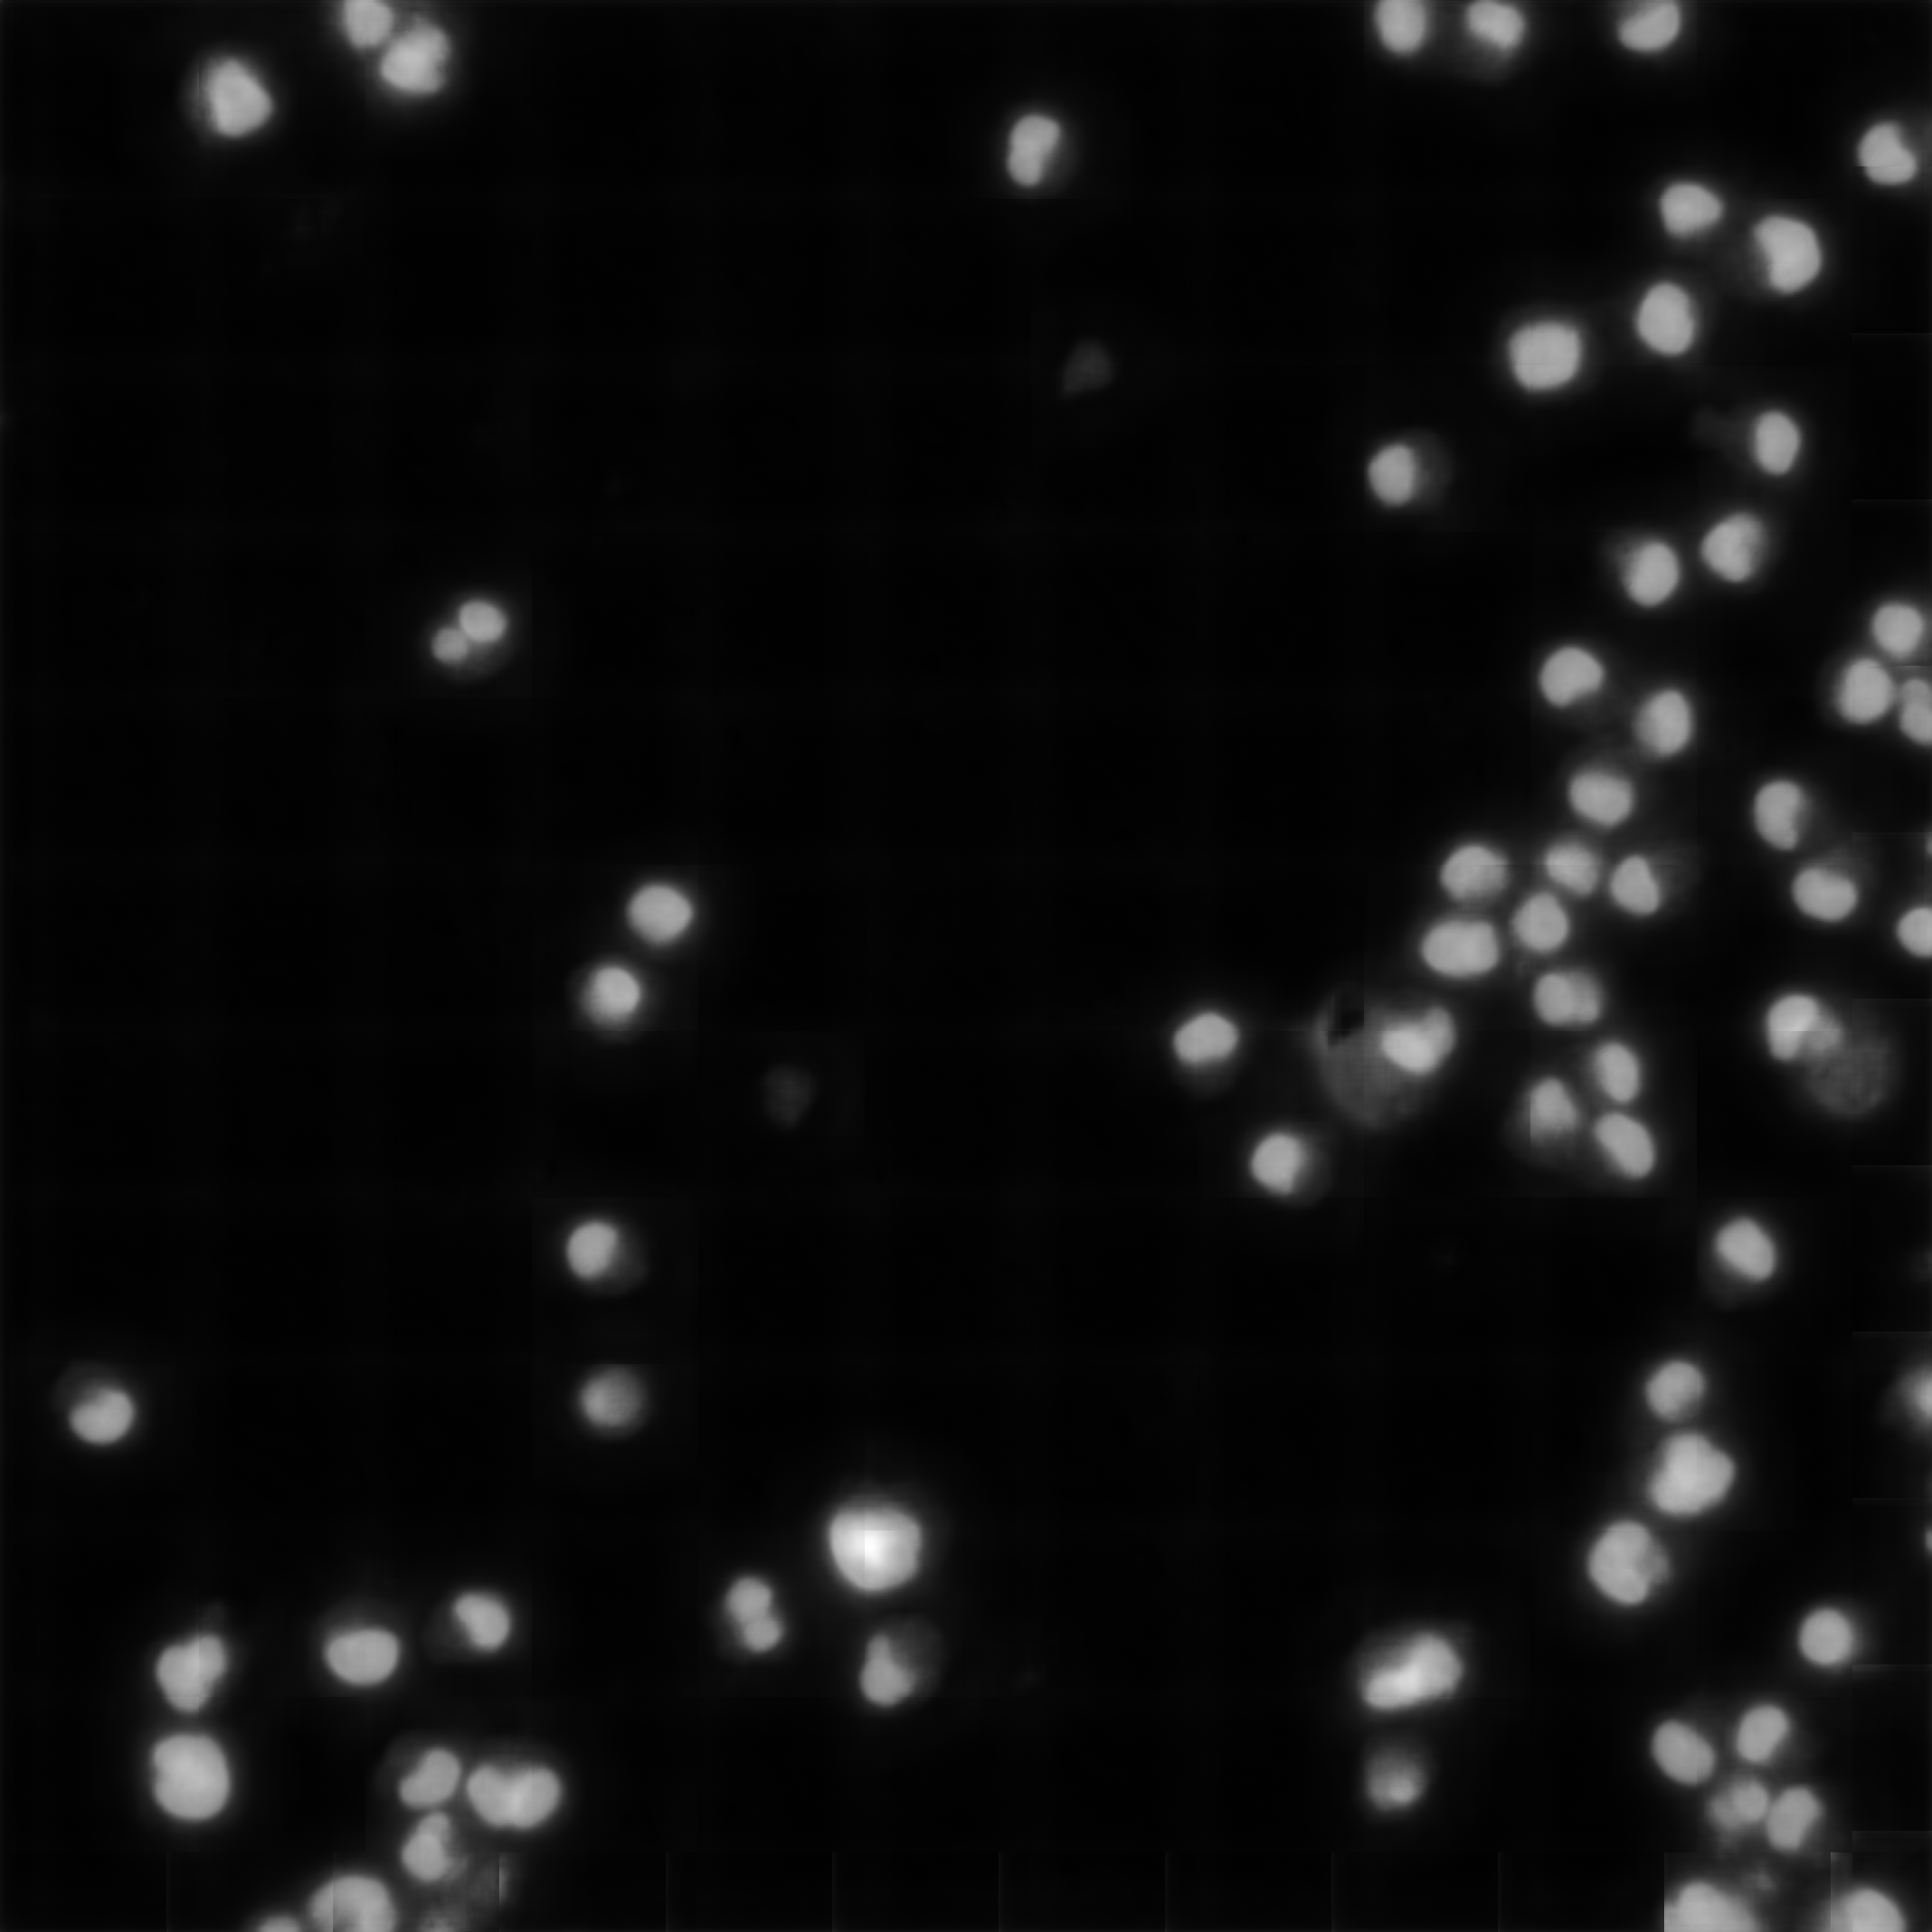
\includegraphics{bilder/lightning-conditions/lightning-1.png} & 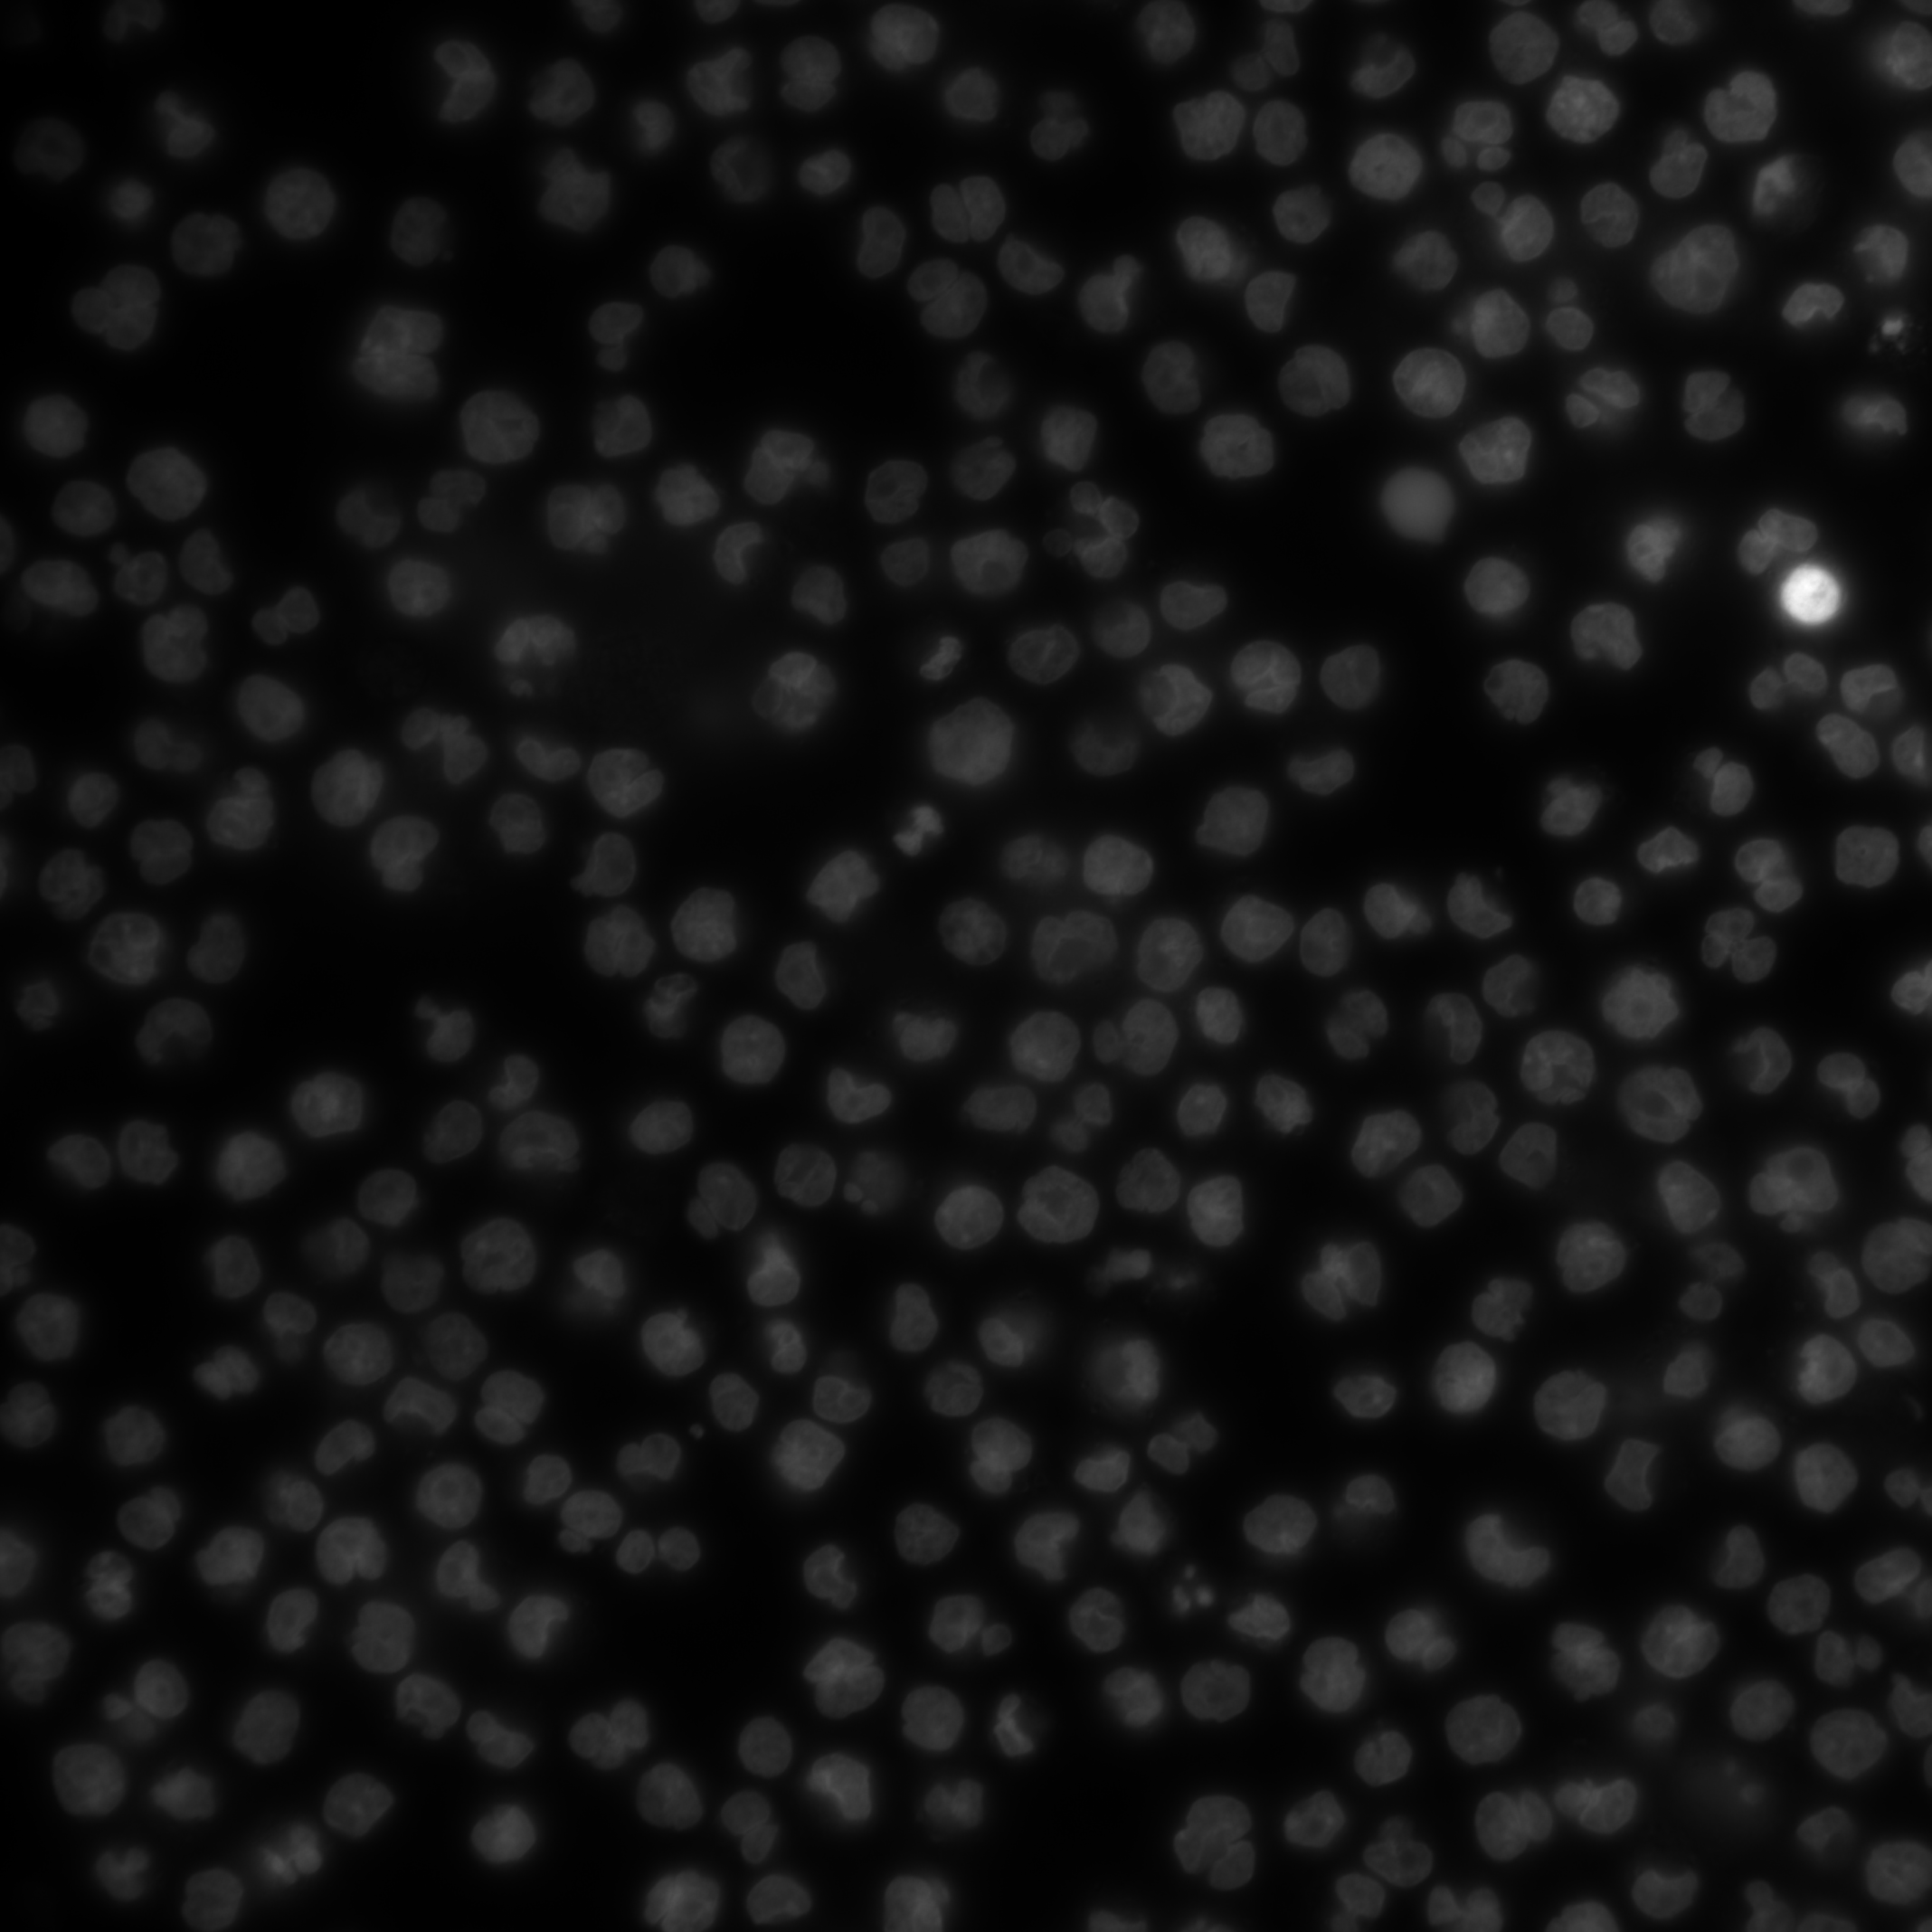
\includegraphics{bilder/lightning-conditions/lightning-2.png} &
            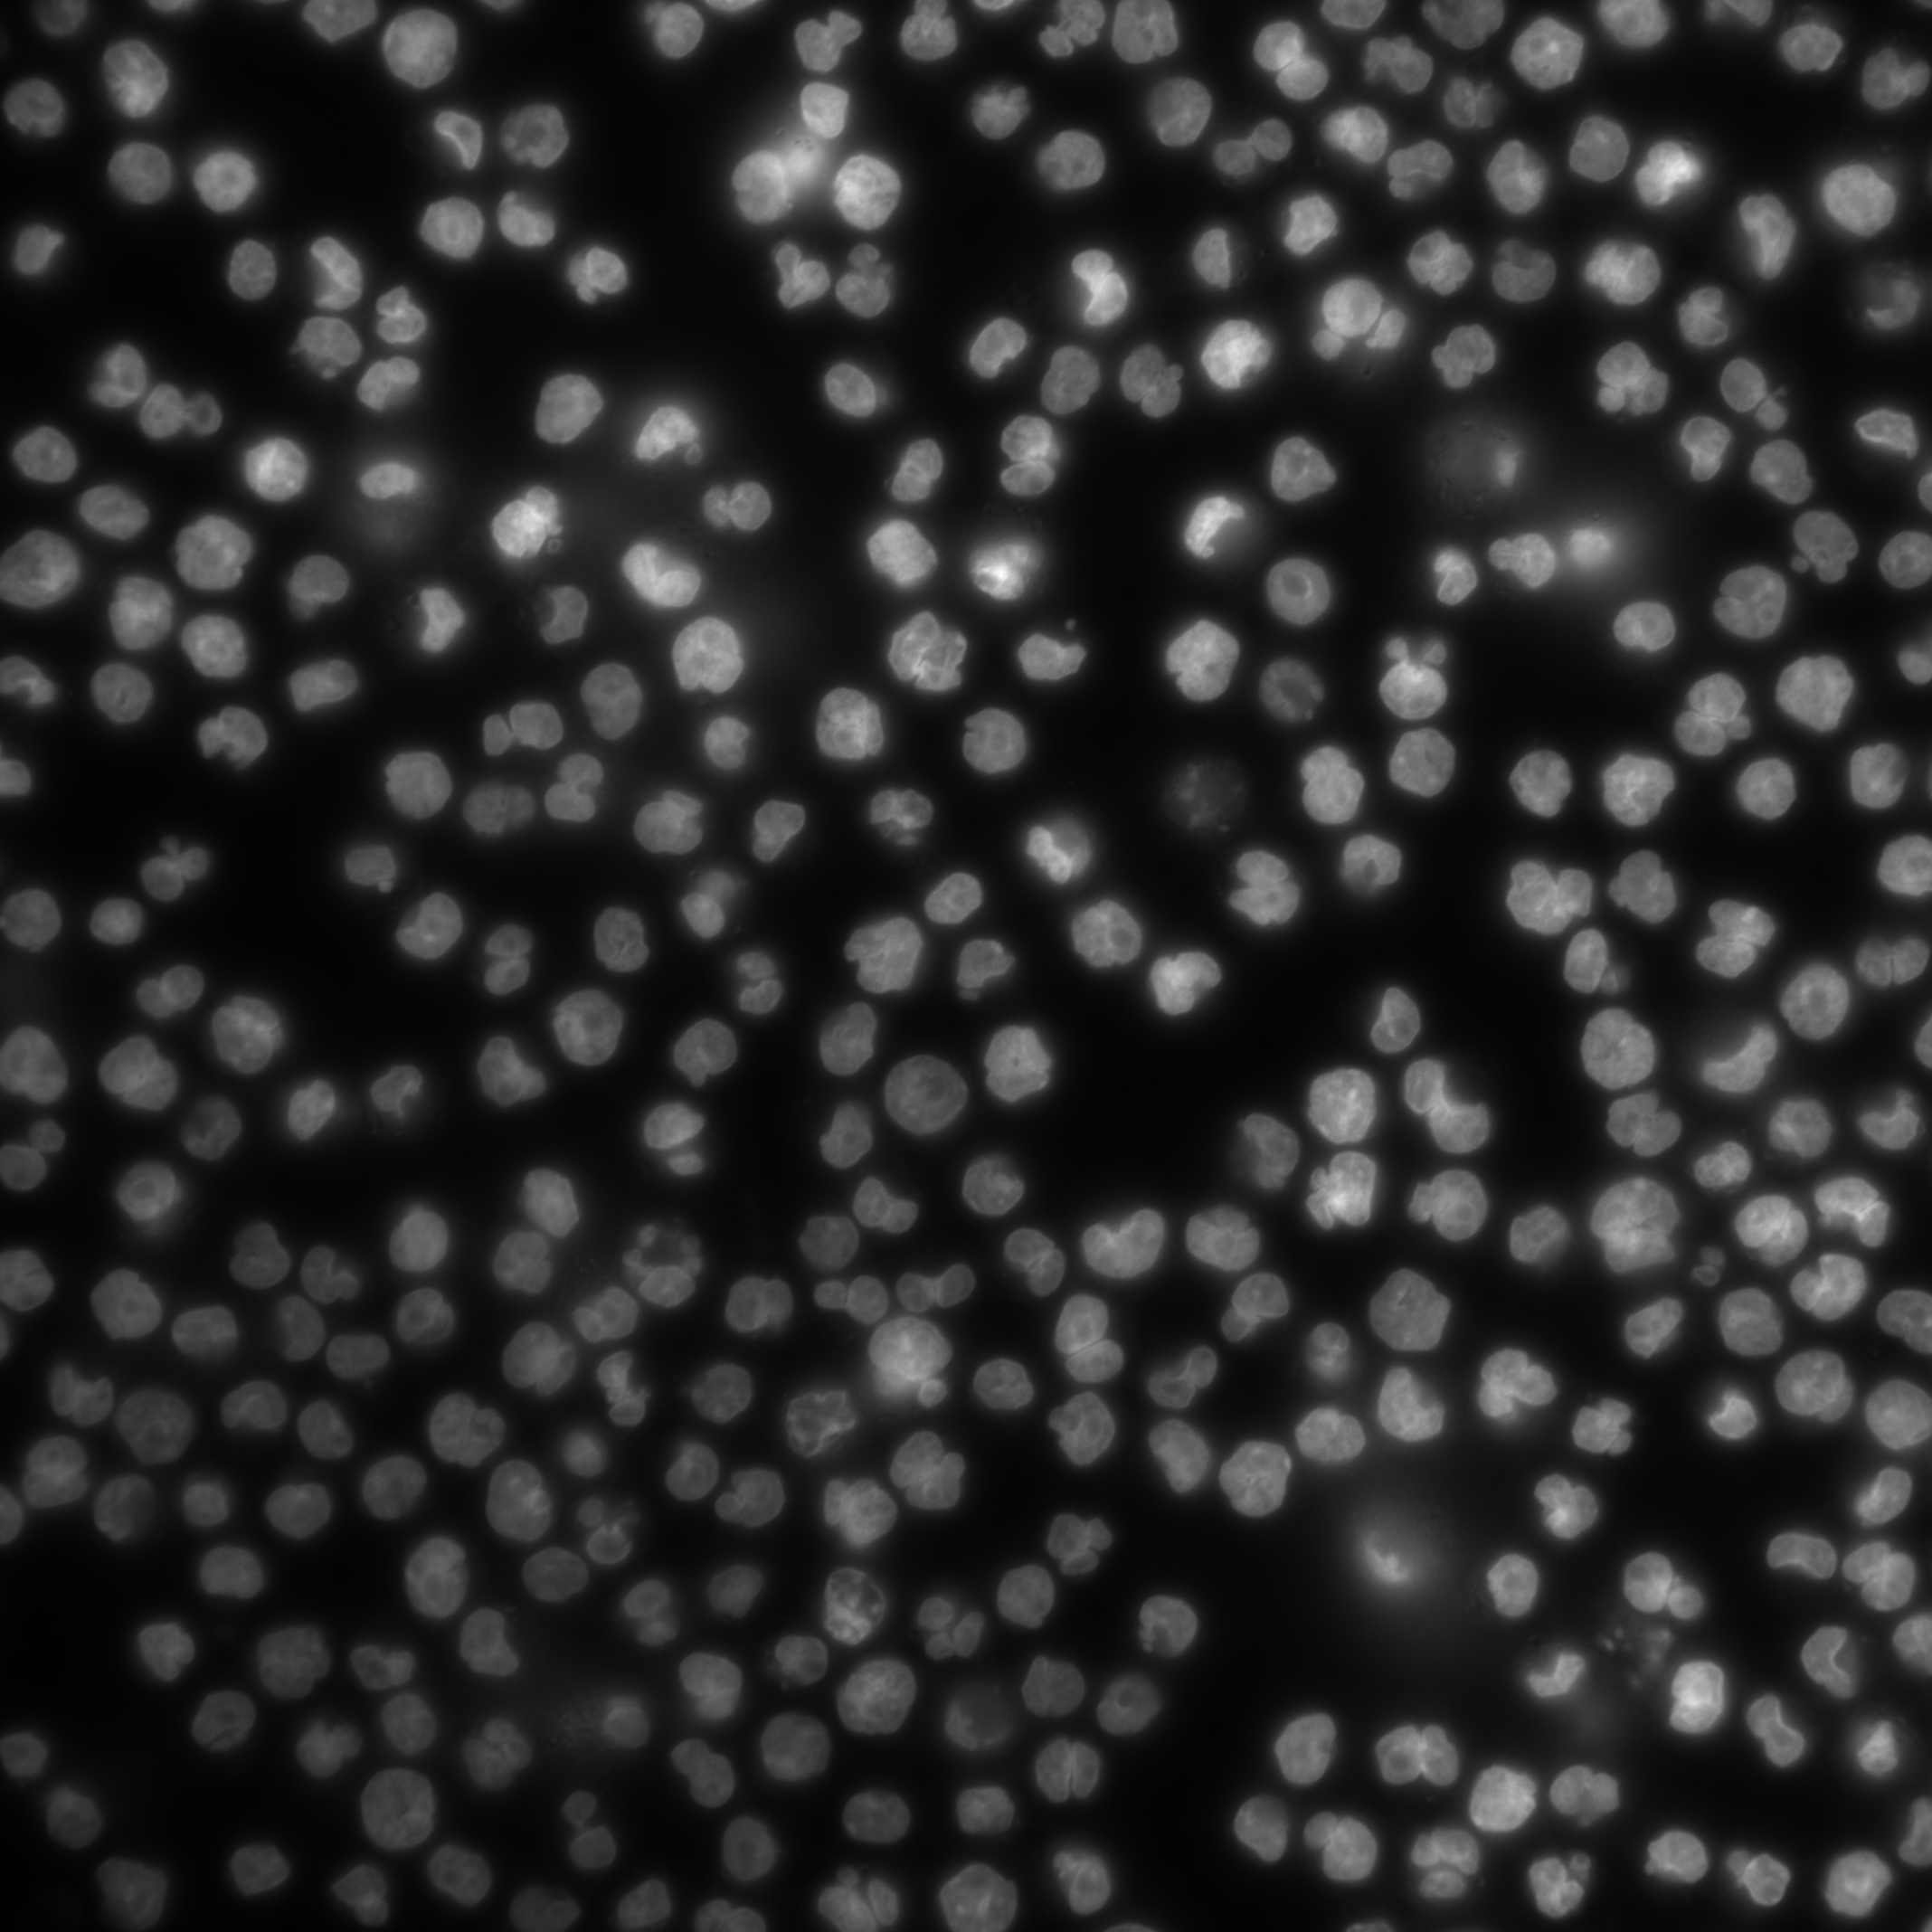
\includegraphics{bilder/lightning-conditions/lightning-3.png} & 
            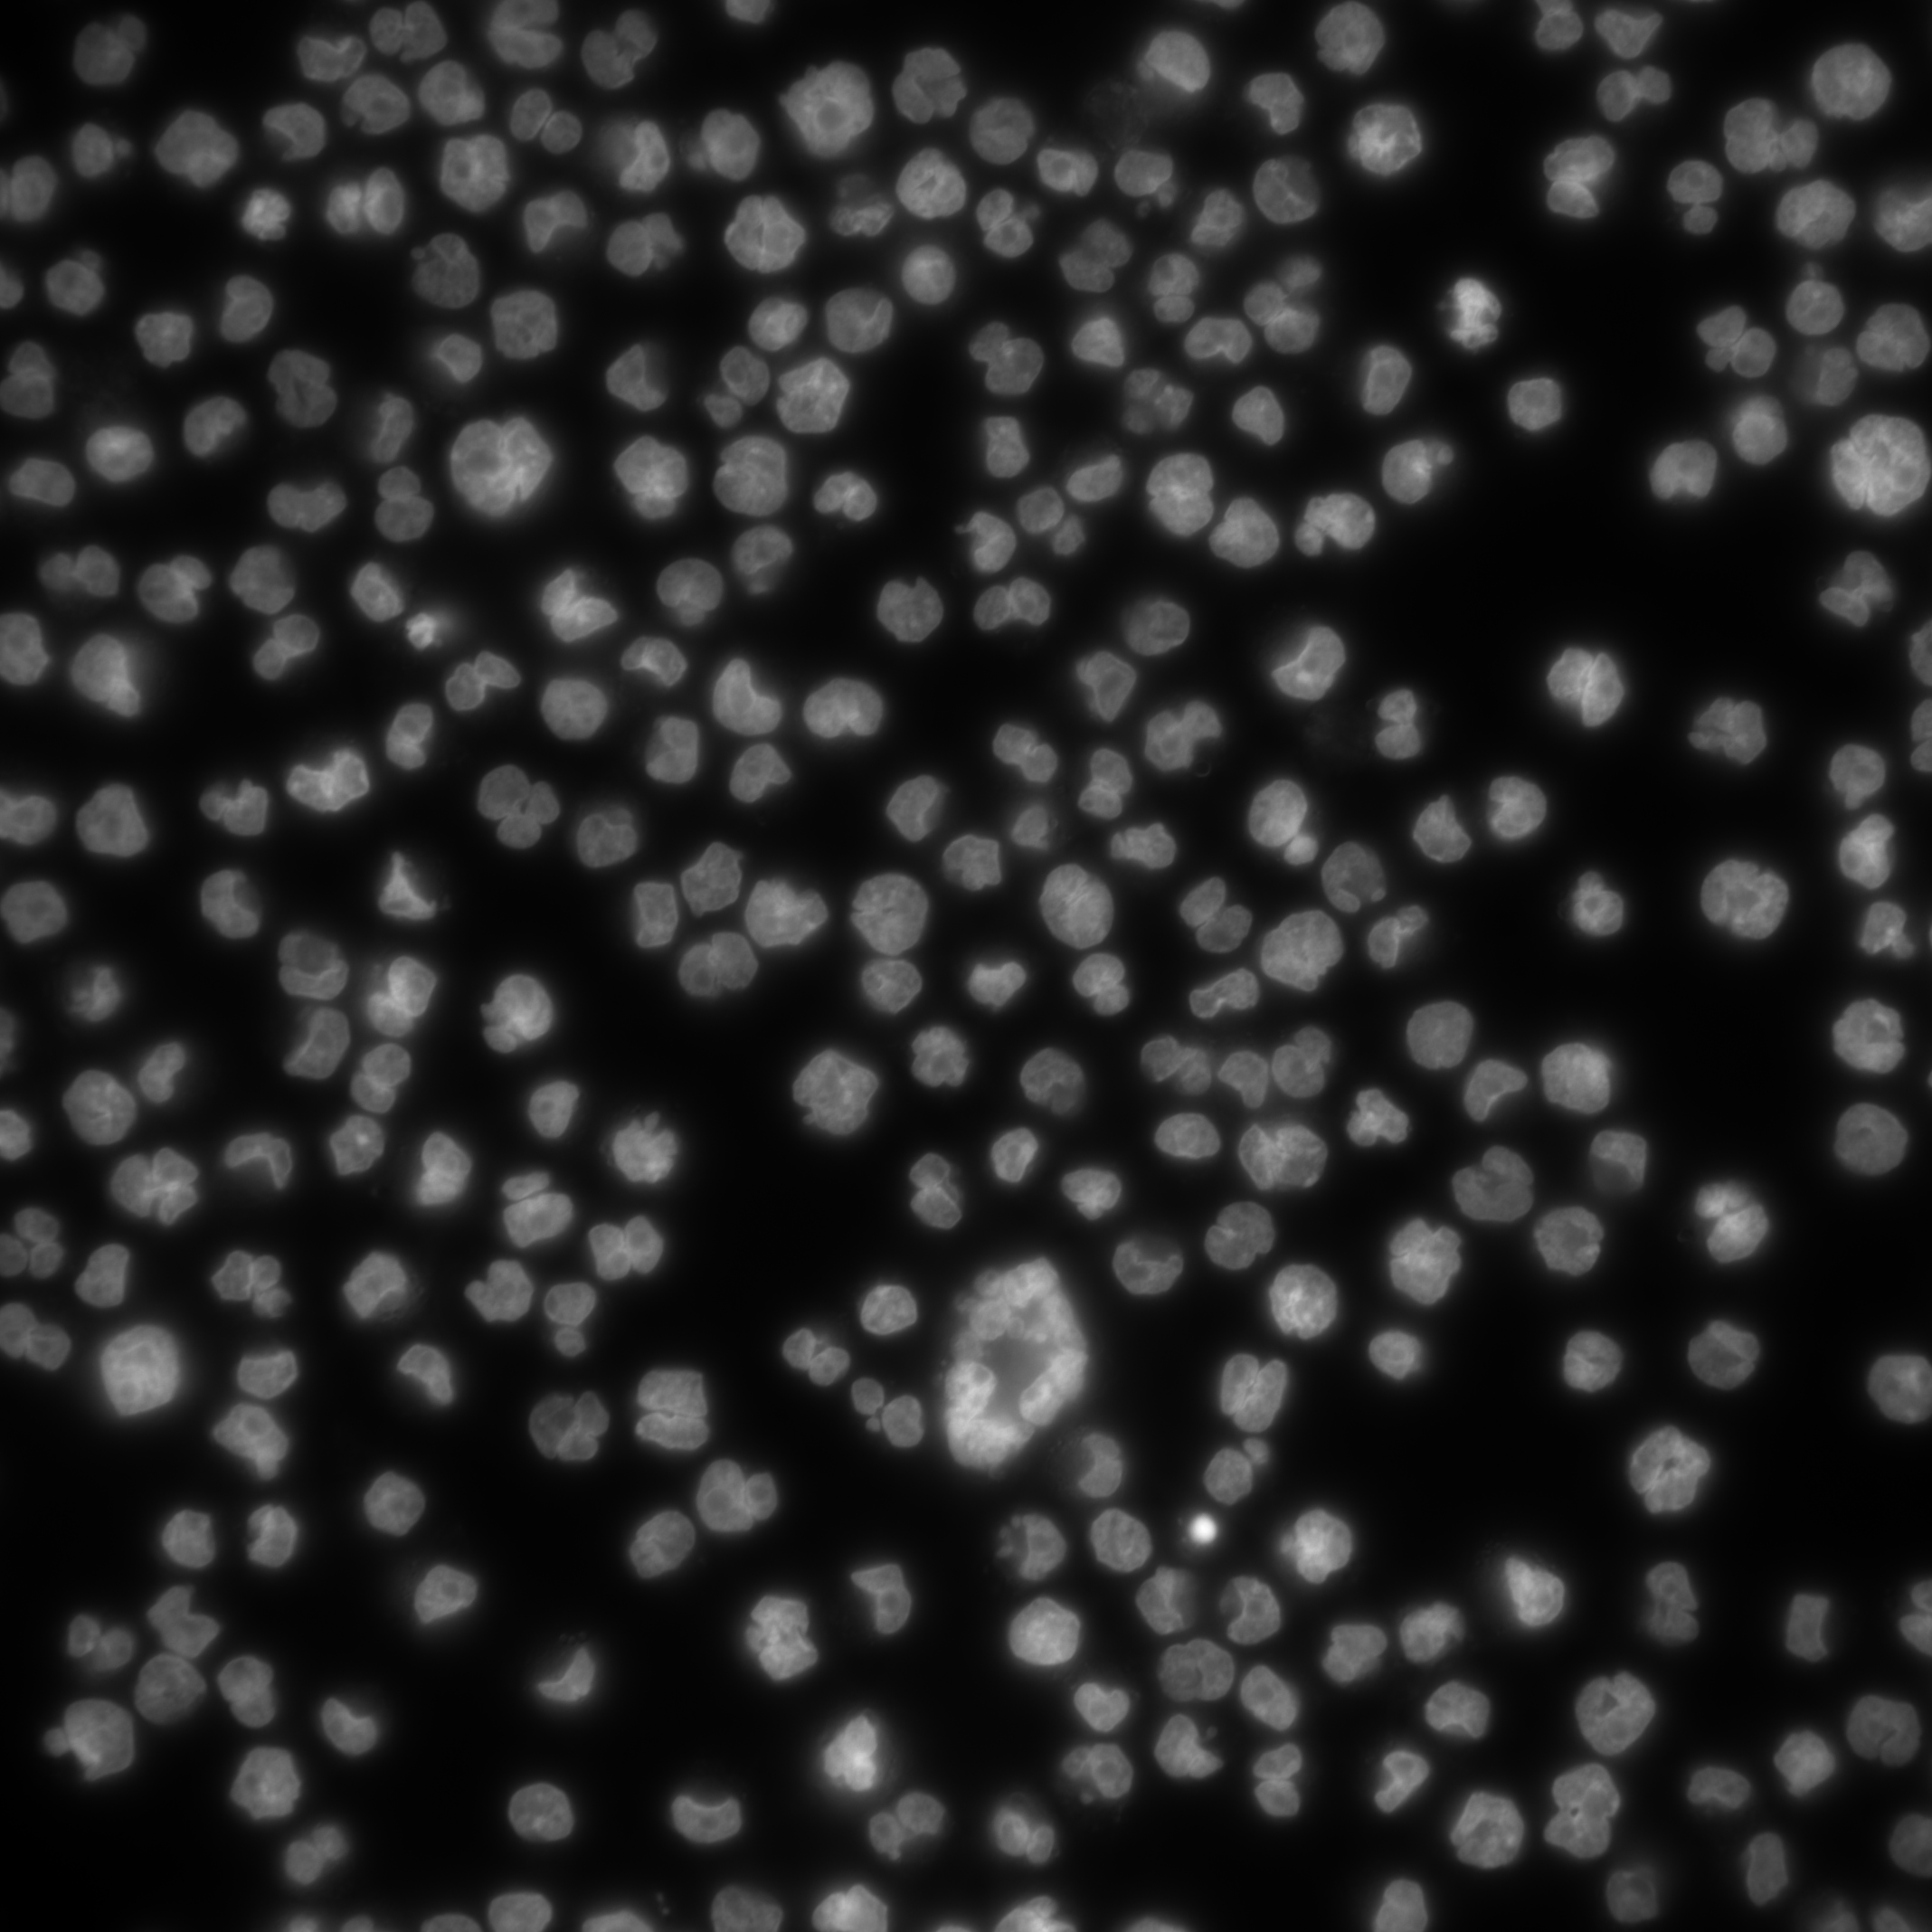
\includegraphics{bilder/lightning-conditions/lightning-4.png}
        \end{tabularx}
    \caption{Different lightning conditions}
    \label{fig:lightning_conditions}
\end{figure}

For example, different brightness of the images that comes from different exposure during the photo taking process might make the nuclei segmentation more challenging. The same goes for the different lighting conditions. Different lighning conditions are presented in Figure \ref{fig:lightning_conditions}. The following inconsistenties in lightning conditions are presented (from left to right): image contains too few cells, which leads to background being much darker than usually; overexposure of one cell, which leads to difficulties of segmenting the rest of the cells as they are hard distinguishable from the background; lighting gradient from darker (left bottom corner) to brighter (upper right corner) region; normal lighting conditions.

Another challenge for segmentation bring nuclei that are very close to each other. This might happen sometimes because some of the cells are currently in the process of the division. Also when some have already fully divided, they might still be located close to one another. The example of such situation is presented in Figure \ref{fig:closely-located-cells}.


\begin{figure}[H]
    \centering
    \setkeys{Gin}{width=\linewidth}
    \centering
        \begin{tabularx}{\textwidth}{YY}
            \textbf{Original fluorescence} &
            \textbf{Segmentation} \\
            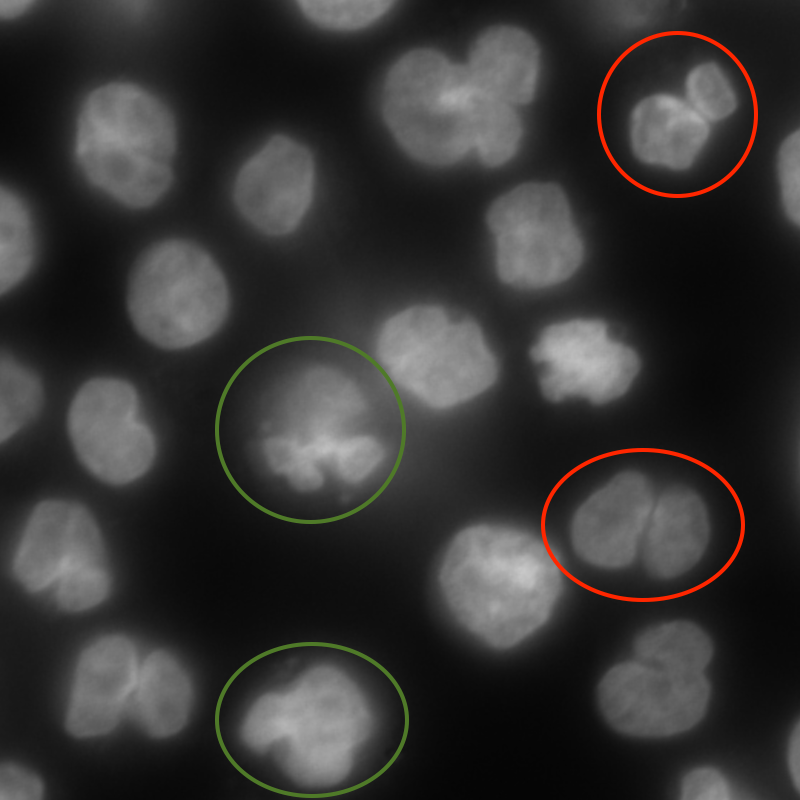
\includegraphics{bilder/close-located-cells/original.png} & 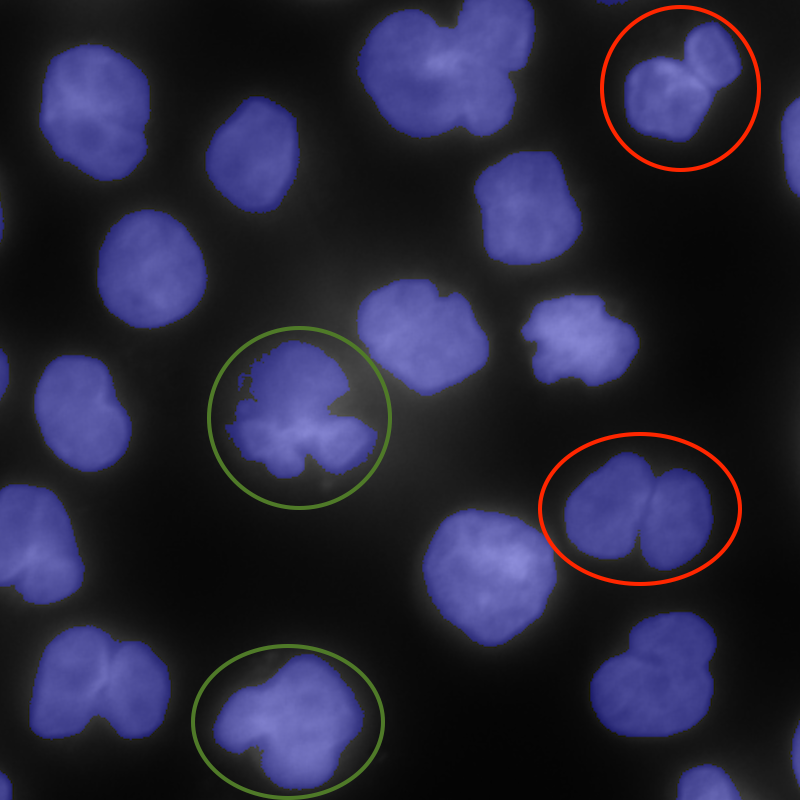
\includegraphics{bilder/close-located-cells/segmented.png}
        \end{tabularx}
    \caption{Closely located cells}
    \label{fig:closely-located-cells}
\end{figure}

Here cells, that are not yet fully divided are highlighted with the green cirles, and ones, that are fully divided, but just located too close to one another are highlighted with red circles. You can see that the segmentation algorithm (described in TODO) recognises both such cases as one cell.

\subsubsection{Thresholding}

Global thresholding is a an algorithm that simply choses one threshold $T$ for the whole histogram of the image. All pixels that are smaller than this threshold $x_i < T$ are assigned to be of class $0$ (background) and all pixels that are larger than this threshold $x_i > T$ are assigned to be of class $1$ (foreground). To find a threshold automatically Gonzalez et al. (cite Digital Image Processing (2nd Edition)) proposed the following algorithm:

\begin{algorithm}
\caption{Global thresholding}\label{alg:global-thresholding}
\begin{algorithmic}
\item 1. Select an initial estimate for $T$.
\item 2. Segment the image using T. This will produce 2 groups of pixels $G_1$ (all pixels $x_i > T$) and $G_2$ (all pixels $x_i < T$).  
\item 3. Computer the average gray values $\mu_1$ and $\mu_2$ for the pixels in  regions $G_1$ and $G_2$.
\item 4. Compute a new threshold value 
    $T' = \frac{\mu_1 + \mu_2}{2}$
\item 5. Repeat steps 2-4 until difference in the change of value $T$ is smaller that a predefined parameter.
\end{algorithmic}
\end{algorithm}

There are different ways of how one can define such initial threshold. There is also no single best solution for all of the cases. For example, when one has an assumption that the foreground occupies approximately the same area as the background, than initial threshold $T$ should be chosen to be an average gray level. In this case global thresholding did not perfom well due to different intensities in different regions of the images (non-uniform illumination). Distribution of the cells also varies through the dataset and some images contain more cells, while other contain only few.

In order to segment the background from the foreground (nuclei), the following function was used:

\begin{lstlisting}
    skimage.filters.local_threshold(img, block_size=7, method='gaussian', offset=0)
\end{lstlisting}

This is where basic adaptive thresholding or local thresholding comes in handy. The advantage of this method hides in the fact, that it doesn't compute a threshold based on the full histogram of the image, but uses parts of it to compute different thresholds for different subregions of the image. This method is also known as adaptive or dynamic thresholding. The threshold value is the weighted mean for the local neighborhood of a pixel subtracted by a constant. (cite Digital Image Processing (2nd Edition)). With the image size of 2136x2136, the local neighborhood or a \textit{block size} was chosen equal to 111 by experimenting with different values. The default method used on for local thresholding is \textit{gaussian}. \textit{offset} valut is a constant that will be subtracted from weighted mean of neighborhood during the calculation of the local threshold, by default this value is $0$. (cite skimage)

Let $z$ be a random variable that quantifies a gray-level value of the pixel, then the histogram of the image is a probability density function (PDF) $p(z)$. Since we assume that the image contains a background and a foreground, then this PDF is a mixture of two densities $p_1(z)$ and $p_@(z)$ weighted by the relative areas of these two classes (their number of pixels) $P_1$ and $P_2$. Then 

\begin{equation}
    p(z) = P_1 p_1(z) + P_2 p_2(z)
\end{equation}

By assuming Gauassian model for both $p_1(z)$ and $p_2(z)$, one gets a Gaussian Mixture Model (GMM). Here since we assume that each pixel can be asssigned to background of foreground only, we have $P_1 + P_2 = 1$. 

\begin{figure}[htb]
	\begin{center}
		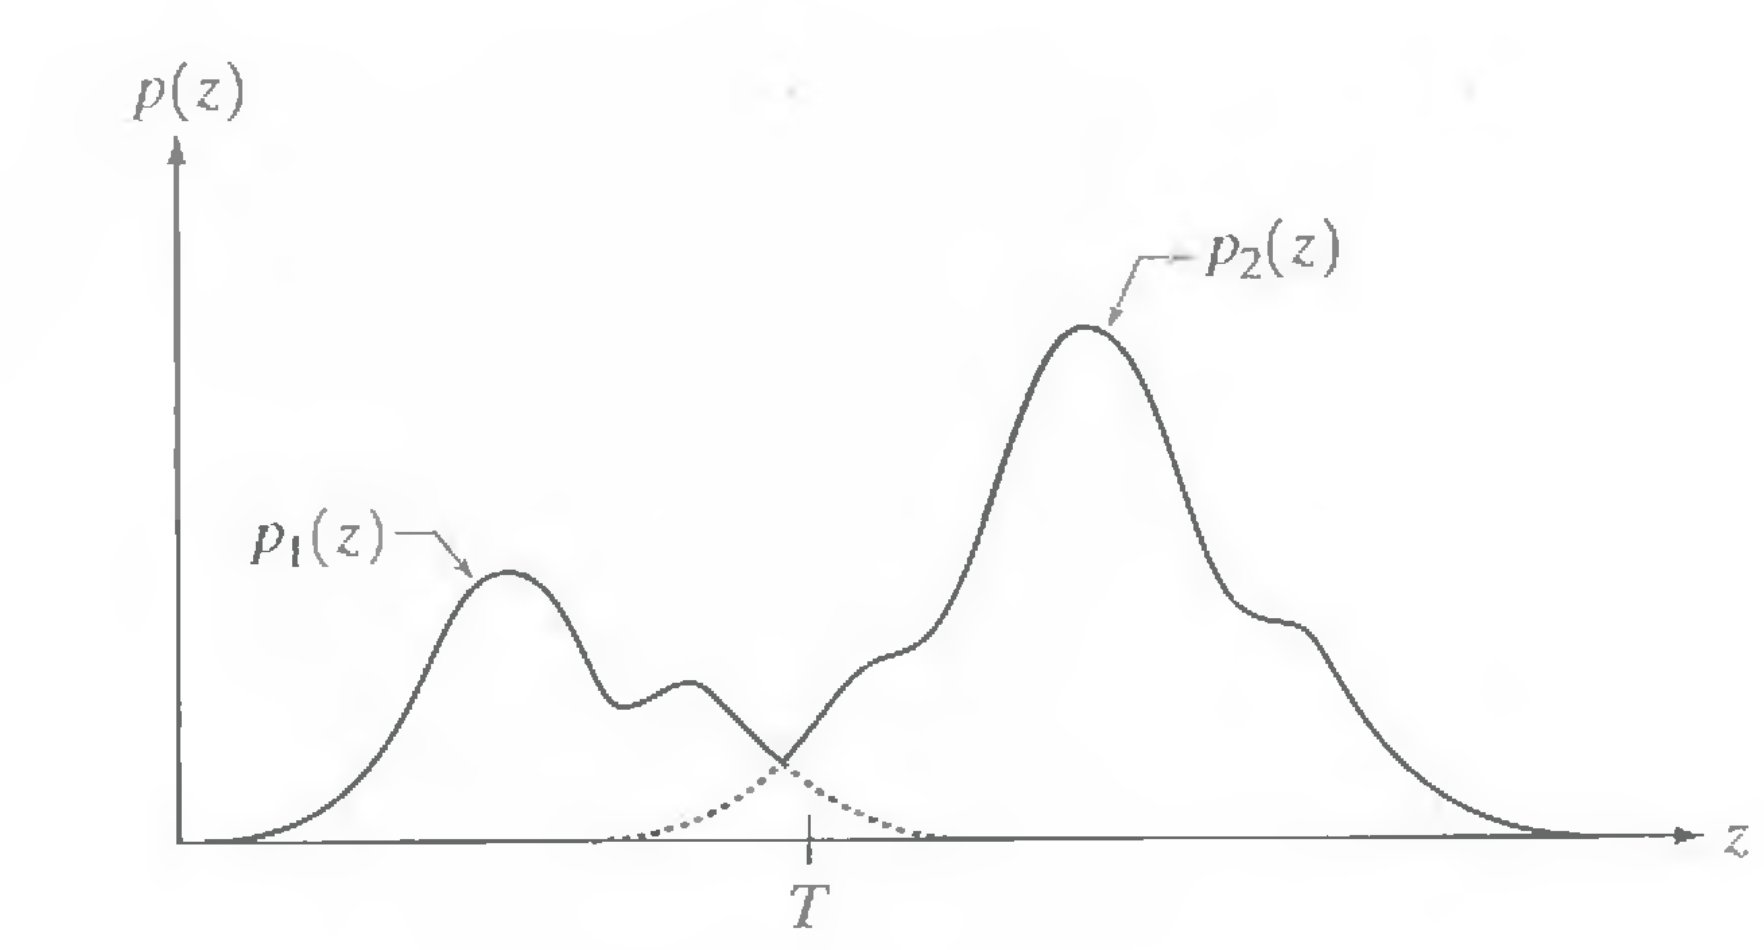
\includegraphics[width=0.8\linewidth]{bilder/Gonzalez.png}
		\caption{Histogram as a probability density function}\label{fig:gmm}
	\end{center}
\end{figure}

Probability to falsely classify an background pixel as object then is:

\begin{equation}
    E_1(T) = \int_{-\infty}^T{p_2(z) \, dz}
\end{equation}

And probability to falsely classify an object pixel as background then is:

\begin{equation}
    E_2(T) = \int_T^{+\infty}{p_1(z) \, dz}
\end{equation}

The overall error is:

\begin{equation}
    E(T) = P_1E_1(T) + P_2E_2(T)
\end{equation}

By differentiating $E(T)$ wrt to $T$ and equating the result to zero the optmal equation will be:

\begin{equation}
    P_1p_1(T) = P_2p_2(T)
\end{equation}

Since Gaussian distributions have been assumed then:
\begin{equation}
    p(z) = \frac{P_1}{\sqrt{2\pi} \sigma_1}e^{-\frac{(z-\mu_1)^2}{2\sigma_1^2}} + \frac{P_2}{\sqrt{2\pi} \sigma_2}e^{-\frac{(z-\mu_2)^2}{2\sigma_2^2}}
\end{equation}

With $\mu_i$ and $\sigma_i^2$ for $i \in \{1, 2\}$ are the mean and variance of the Gaussian distribution $p_i(z)$. This results in the following solution for $T$:
\begin{equation}
    AT^2 + BT + C = 0
\end{equation}

where 

\begin{equation}
    \begin{split}
        &A = \sigma_1^2 + \sigma_2^2 \\
        &B = 2(\mu_1 \sigma_1^2 - \mu_2 \sigma_2^2) \\
        &C = \sigma_1^2 \mu_2^2 - \sigma_2^2 \mu_1^2 + 2\sigma_1^2 2\sigma_2^2ln\left(\frac{\sigma_2P_1}{\sigma_1P_2}\right)
    \end{split}
\end{equation}

To escape two optimal solutions of the quadratic equation it may be assumed that $\sigma_1 = \sigma_2 = \sigma$ and then:

\begin{equation}
    T = \frac{\mu_1 + \mu_2}{2} + \frac{\sigma^2}{\mu_1 - \mu_2}ln\left(\frac{P_2}{P_1}\right)
\end{equation}

Such threshold search is then applied to all of the subregions of the image with overlaps. Threshold are calculated only for the regions that contain two peaks and interpolated to the other pixels from the regions that do not contain clear two peaks in their histograms. If the subregions doesn't contain two peaks, it simply means that there is no foreground or background object on it. 

Of course local thresholding approach takes a longer time:
TODO table with timing. Therefore there as an alternative one can use \textit{minimum thresholding}. This is a global thresholding approach which performs visually a bit worse that a local threshold, however it is much faster (see Table \ref{tab:threshold-timing}).

\begin{table}
\centering
    \begin{tabular}{||c c||} 
     \hline
     Local Threshold & Global Threshold \\ [0.5ex] 
     \hline\hline
     0.3 sec & 17 sec  \\ 
     \hline
    \end{tabular}
    \caption{Threshold timing}
    \label{tab:threshold-timing}
\end{table}

Comparison of the prdections in difficult lightning conditions of minimum thresholding and local adaptive thresholding are presented in the Figure TODO. In extreme cases of difficult lighting conditions the local adaptive thresholding is much better than the minimum thresholding, however on the images of the better quality TODO (see Figure \ref{fig:local-vs-global-normal}) minimum thresholding might successfully sibstitute the local adaptive thresholding when the time of processing is crucial.

\begin{figure}[ht] 
    \begin{subfigure}[b]{0.5\linewidth}
      \centering
      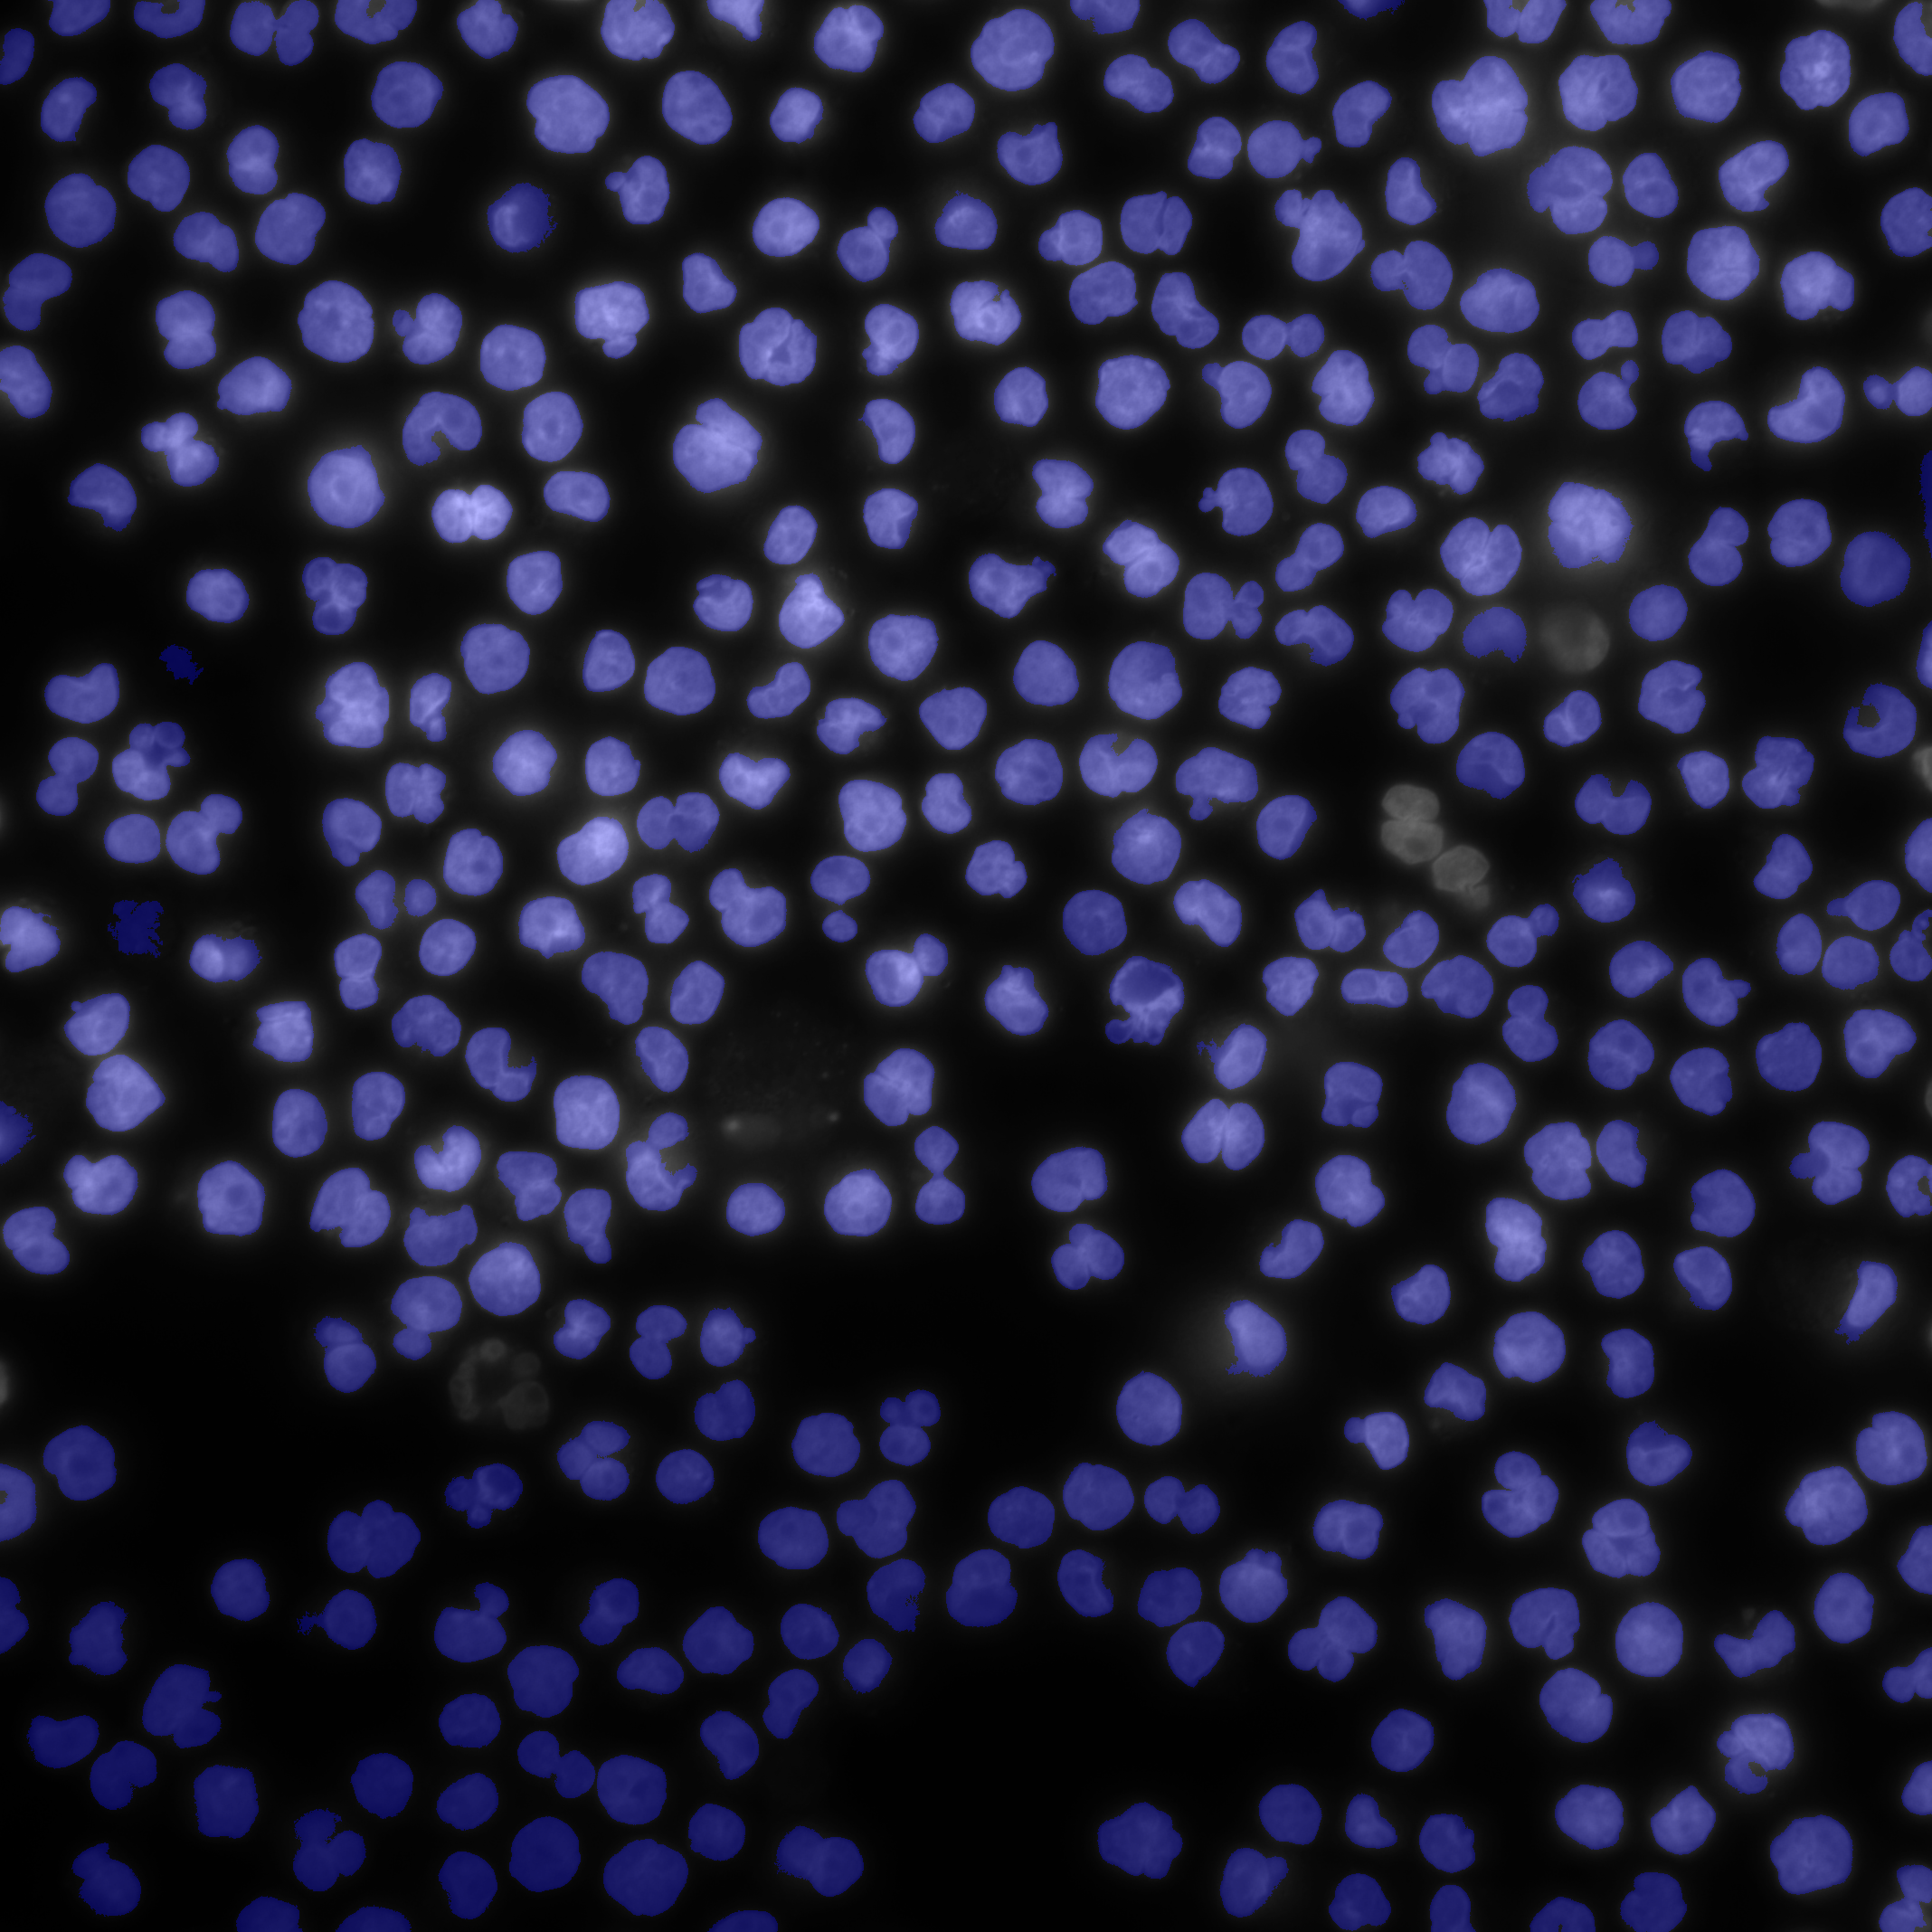
\includegraphics[width=0.75\linewidth]{bilder/difficult-lightning/gradient_local.png} 
      \caption{Local} 
      \label{fig7:a} 
      \vspace{4ex}
    \end{subfigure}%% 
    \begin{subfigure}[b]{0.5\linewidth}
      \centering
      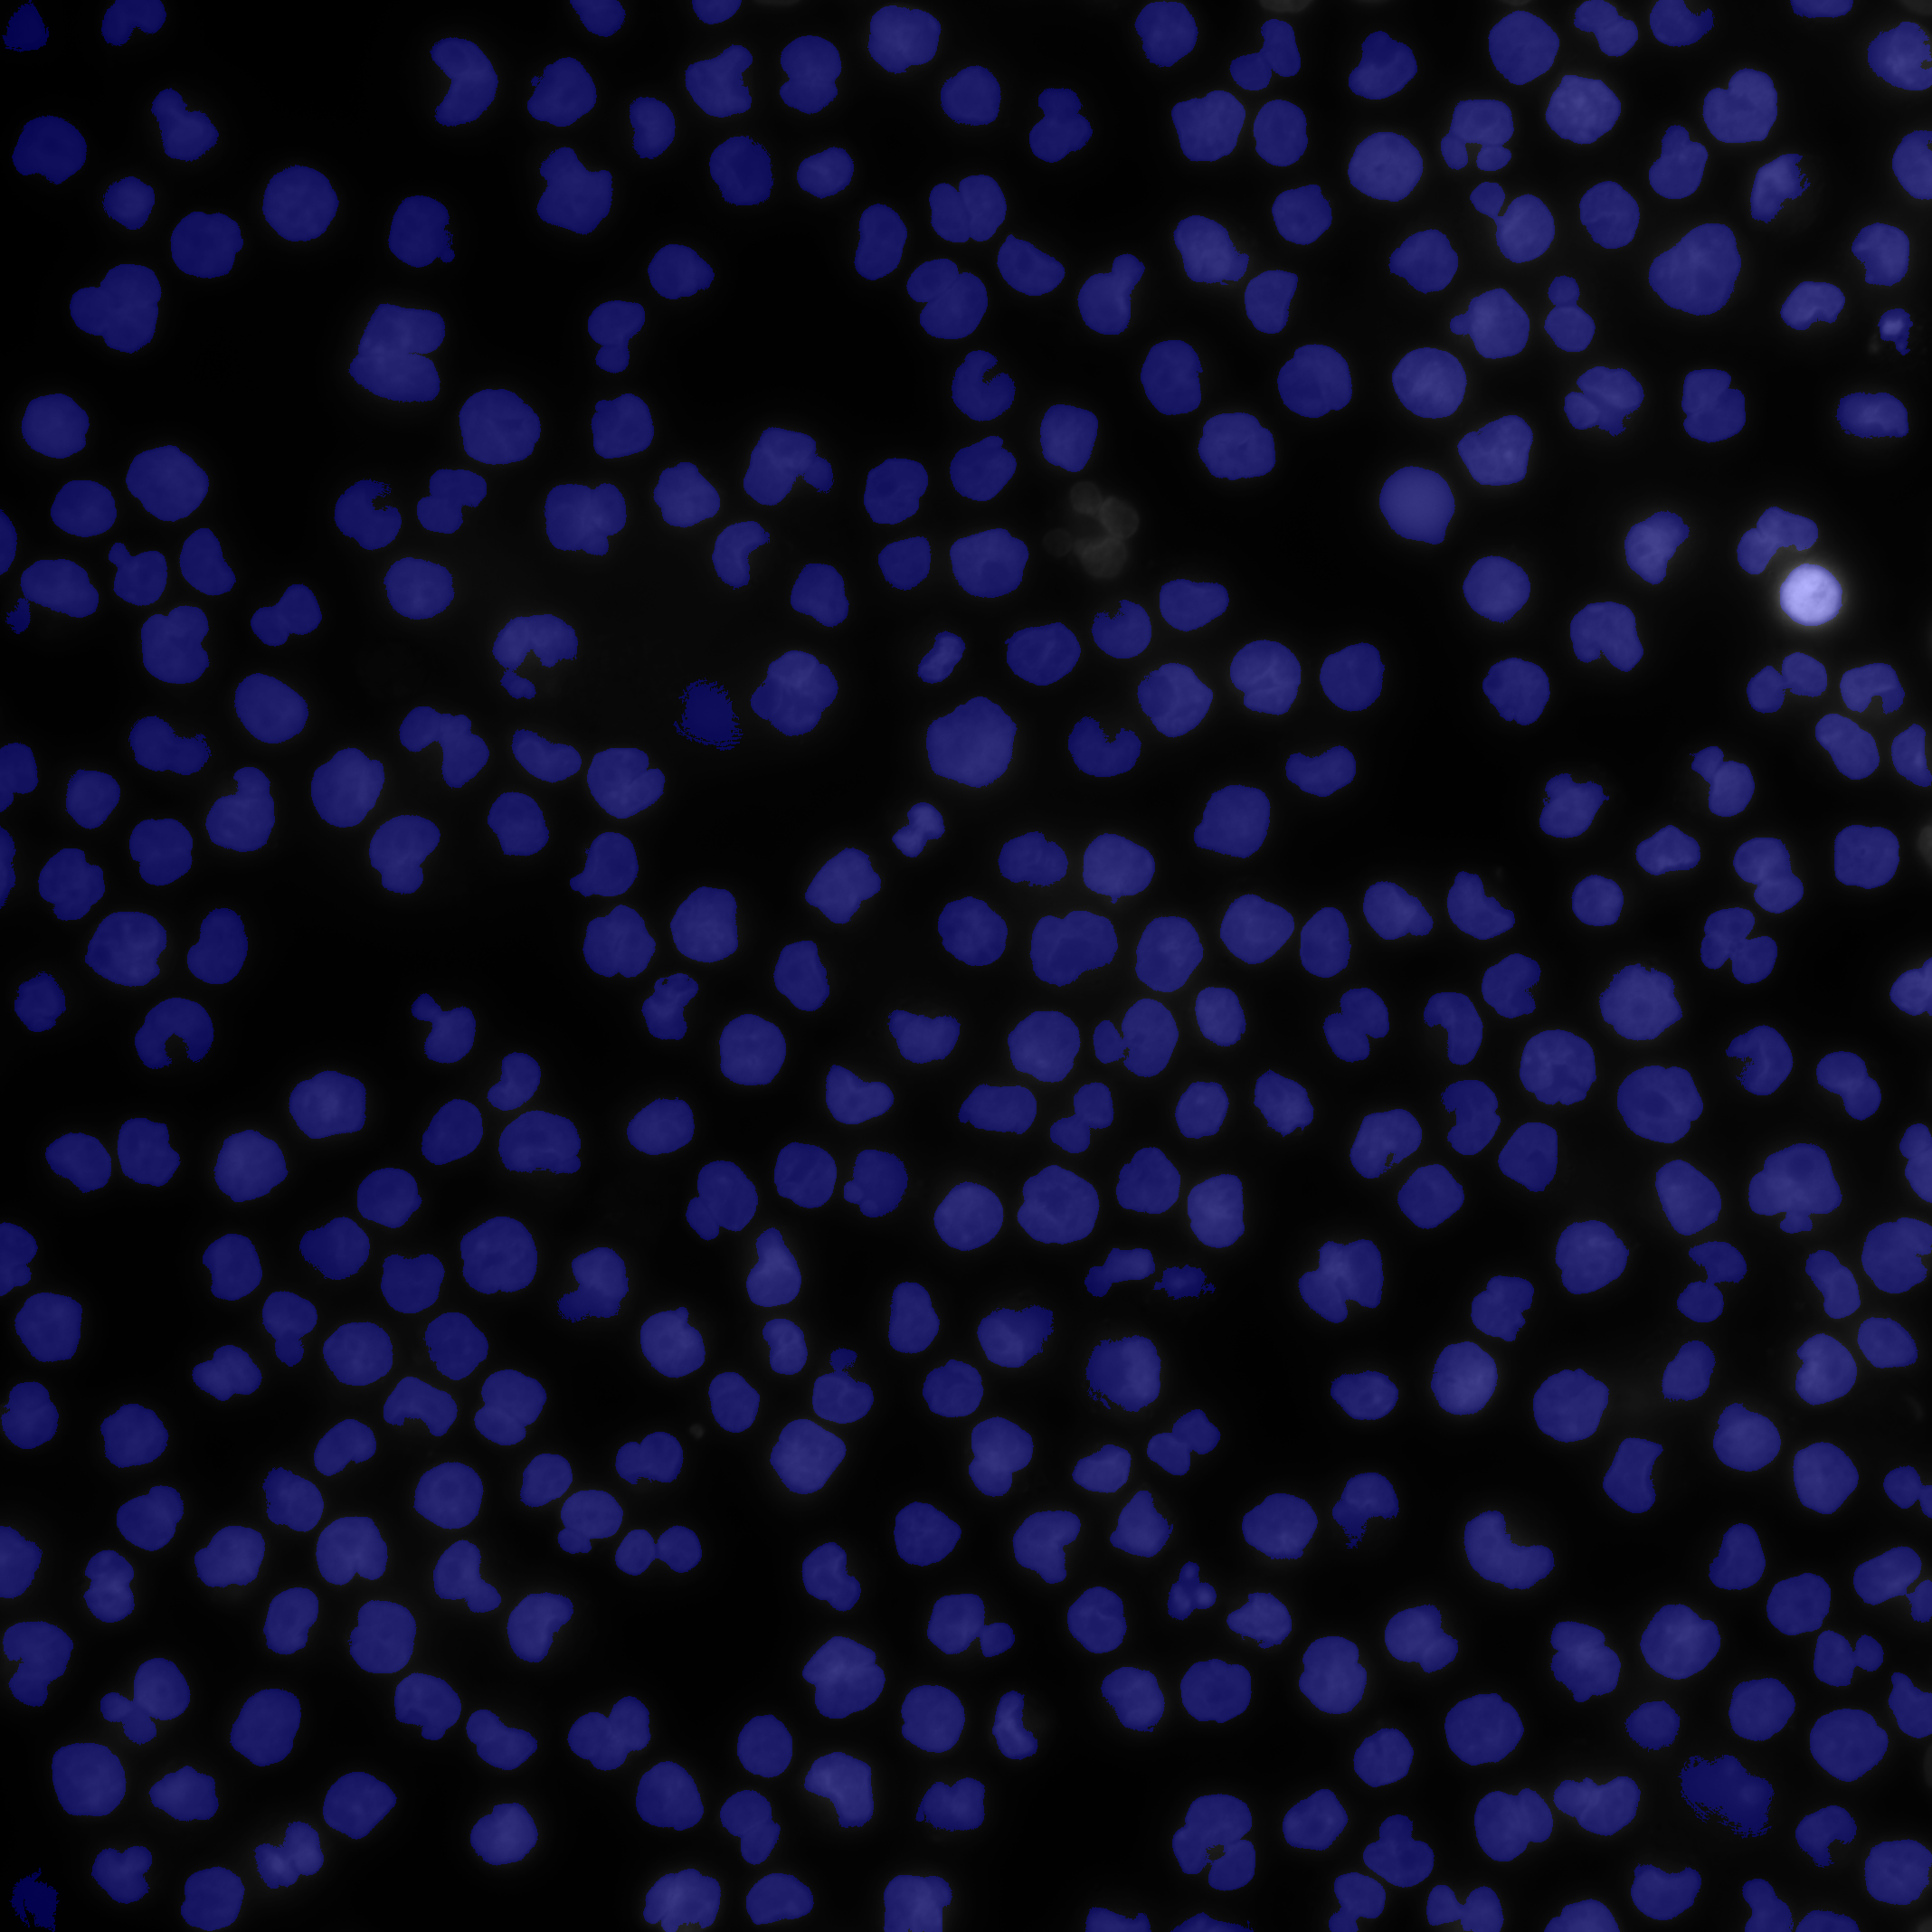
\includegraphics[width=0.75\linewidth]{bilder/difficult-lightning/point_local.png} 
      \caption{Local} 
      \label{fig7:b} 
      \vspace{4ex}
    \end{subfigure} 
    \begin{subfigure}[b]{0.5\linewidth}
      \centering
      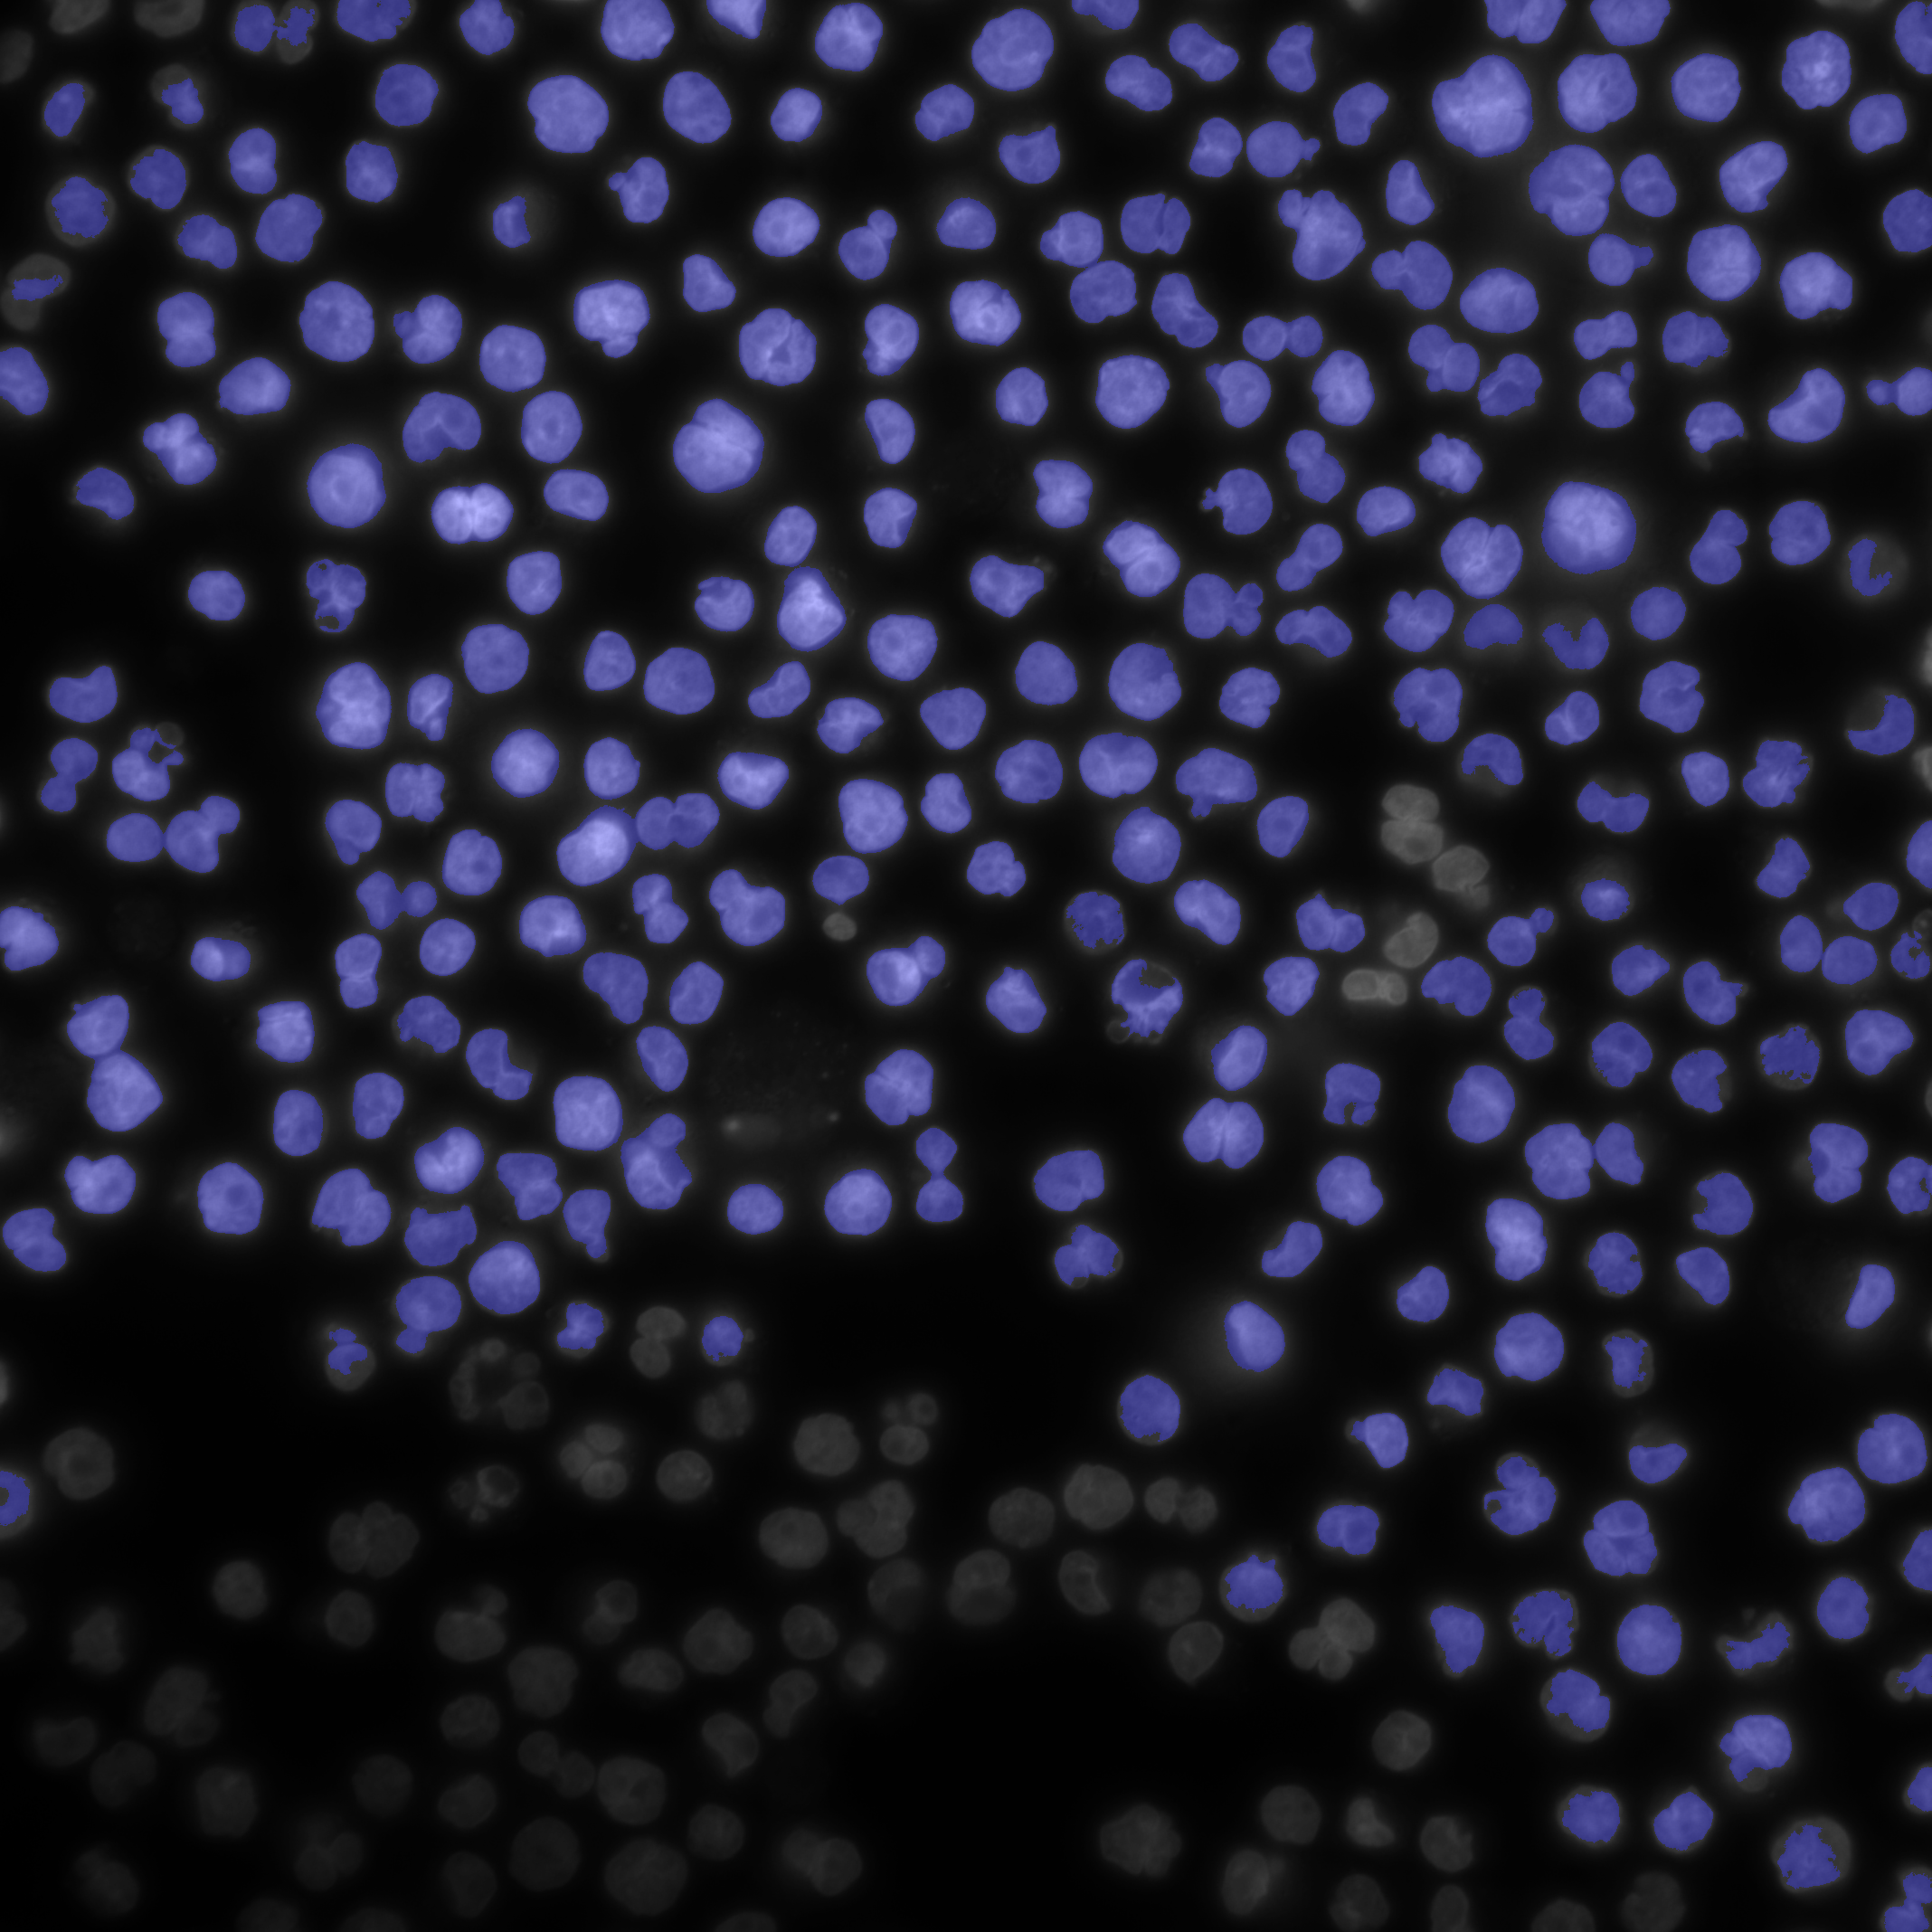
\includegraphics[width=0.75\linewidth]{bilder/difficult-lightning/gradient_min.png} 
      \caption{Global, minimum} 
      \label{fig7:c} 
    \end{subfigure}%%
    \begin{subfigure}[b]{0.5\linewidth}
      \centering
      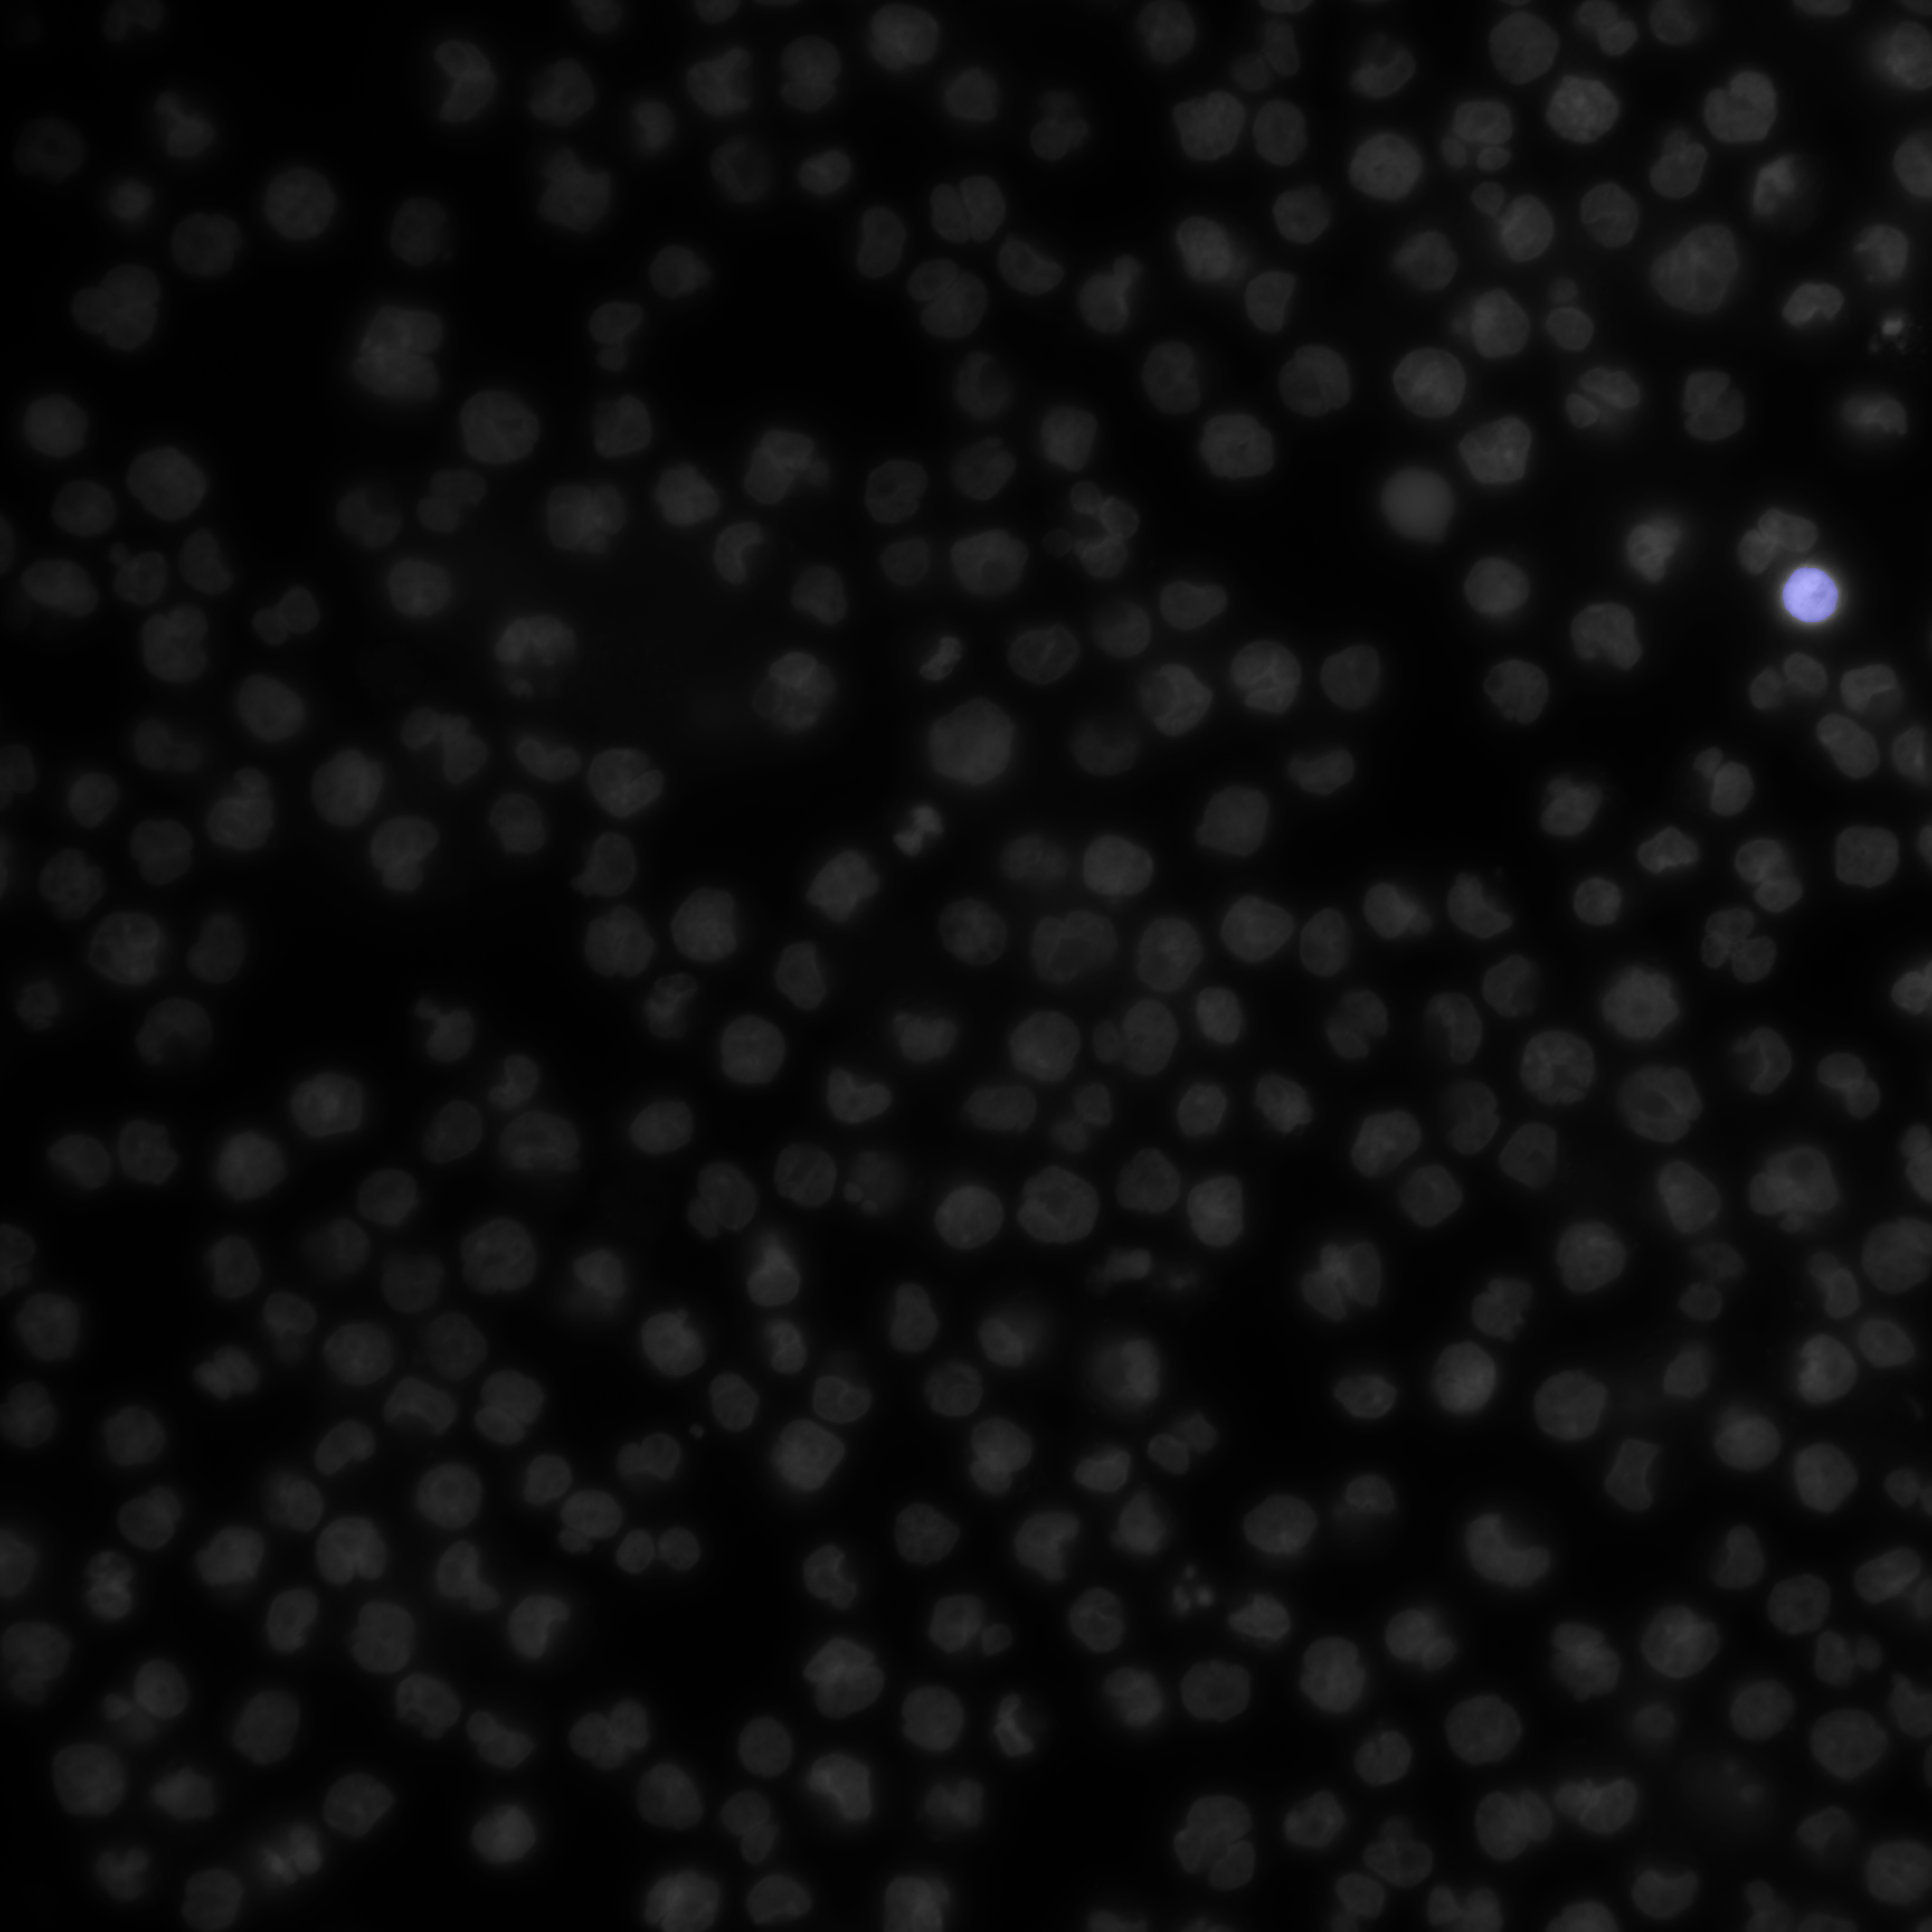
\includegraphics[width=0.75\linewidth]{bilder/difficult-lightning/point_min.png} 
      \caption{Global, minimum} 
      \label{fig7:d} 
    \end{subfigure} 
    \caption{Local vs. Global thresholding}
    \label{fig7} 
\end{figure}

\begin{figure}[H]
    \centering
    \setkeys{Gin}{width=\linewidth}
    \centering
        \begin{tabularx}{\textwidth}{YY}
            \textbf{Local thresholding} &
            \textbf{Minimum thresholding} \\
            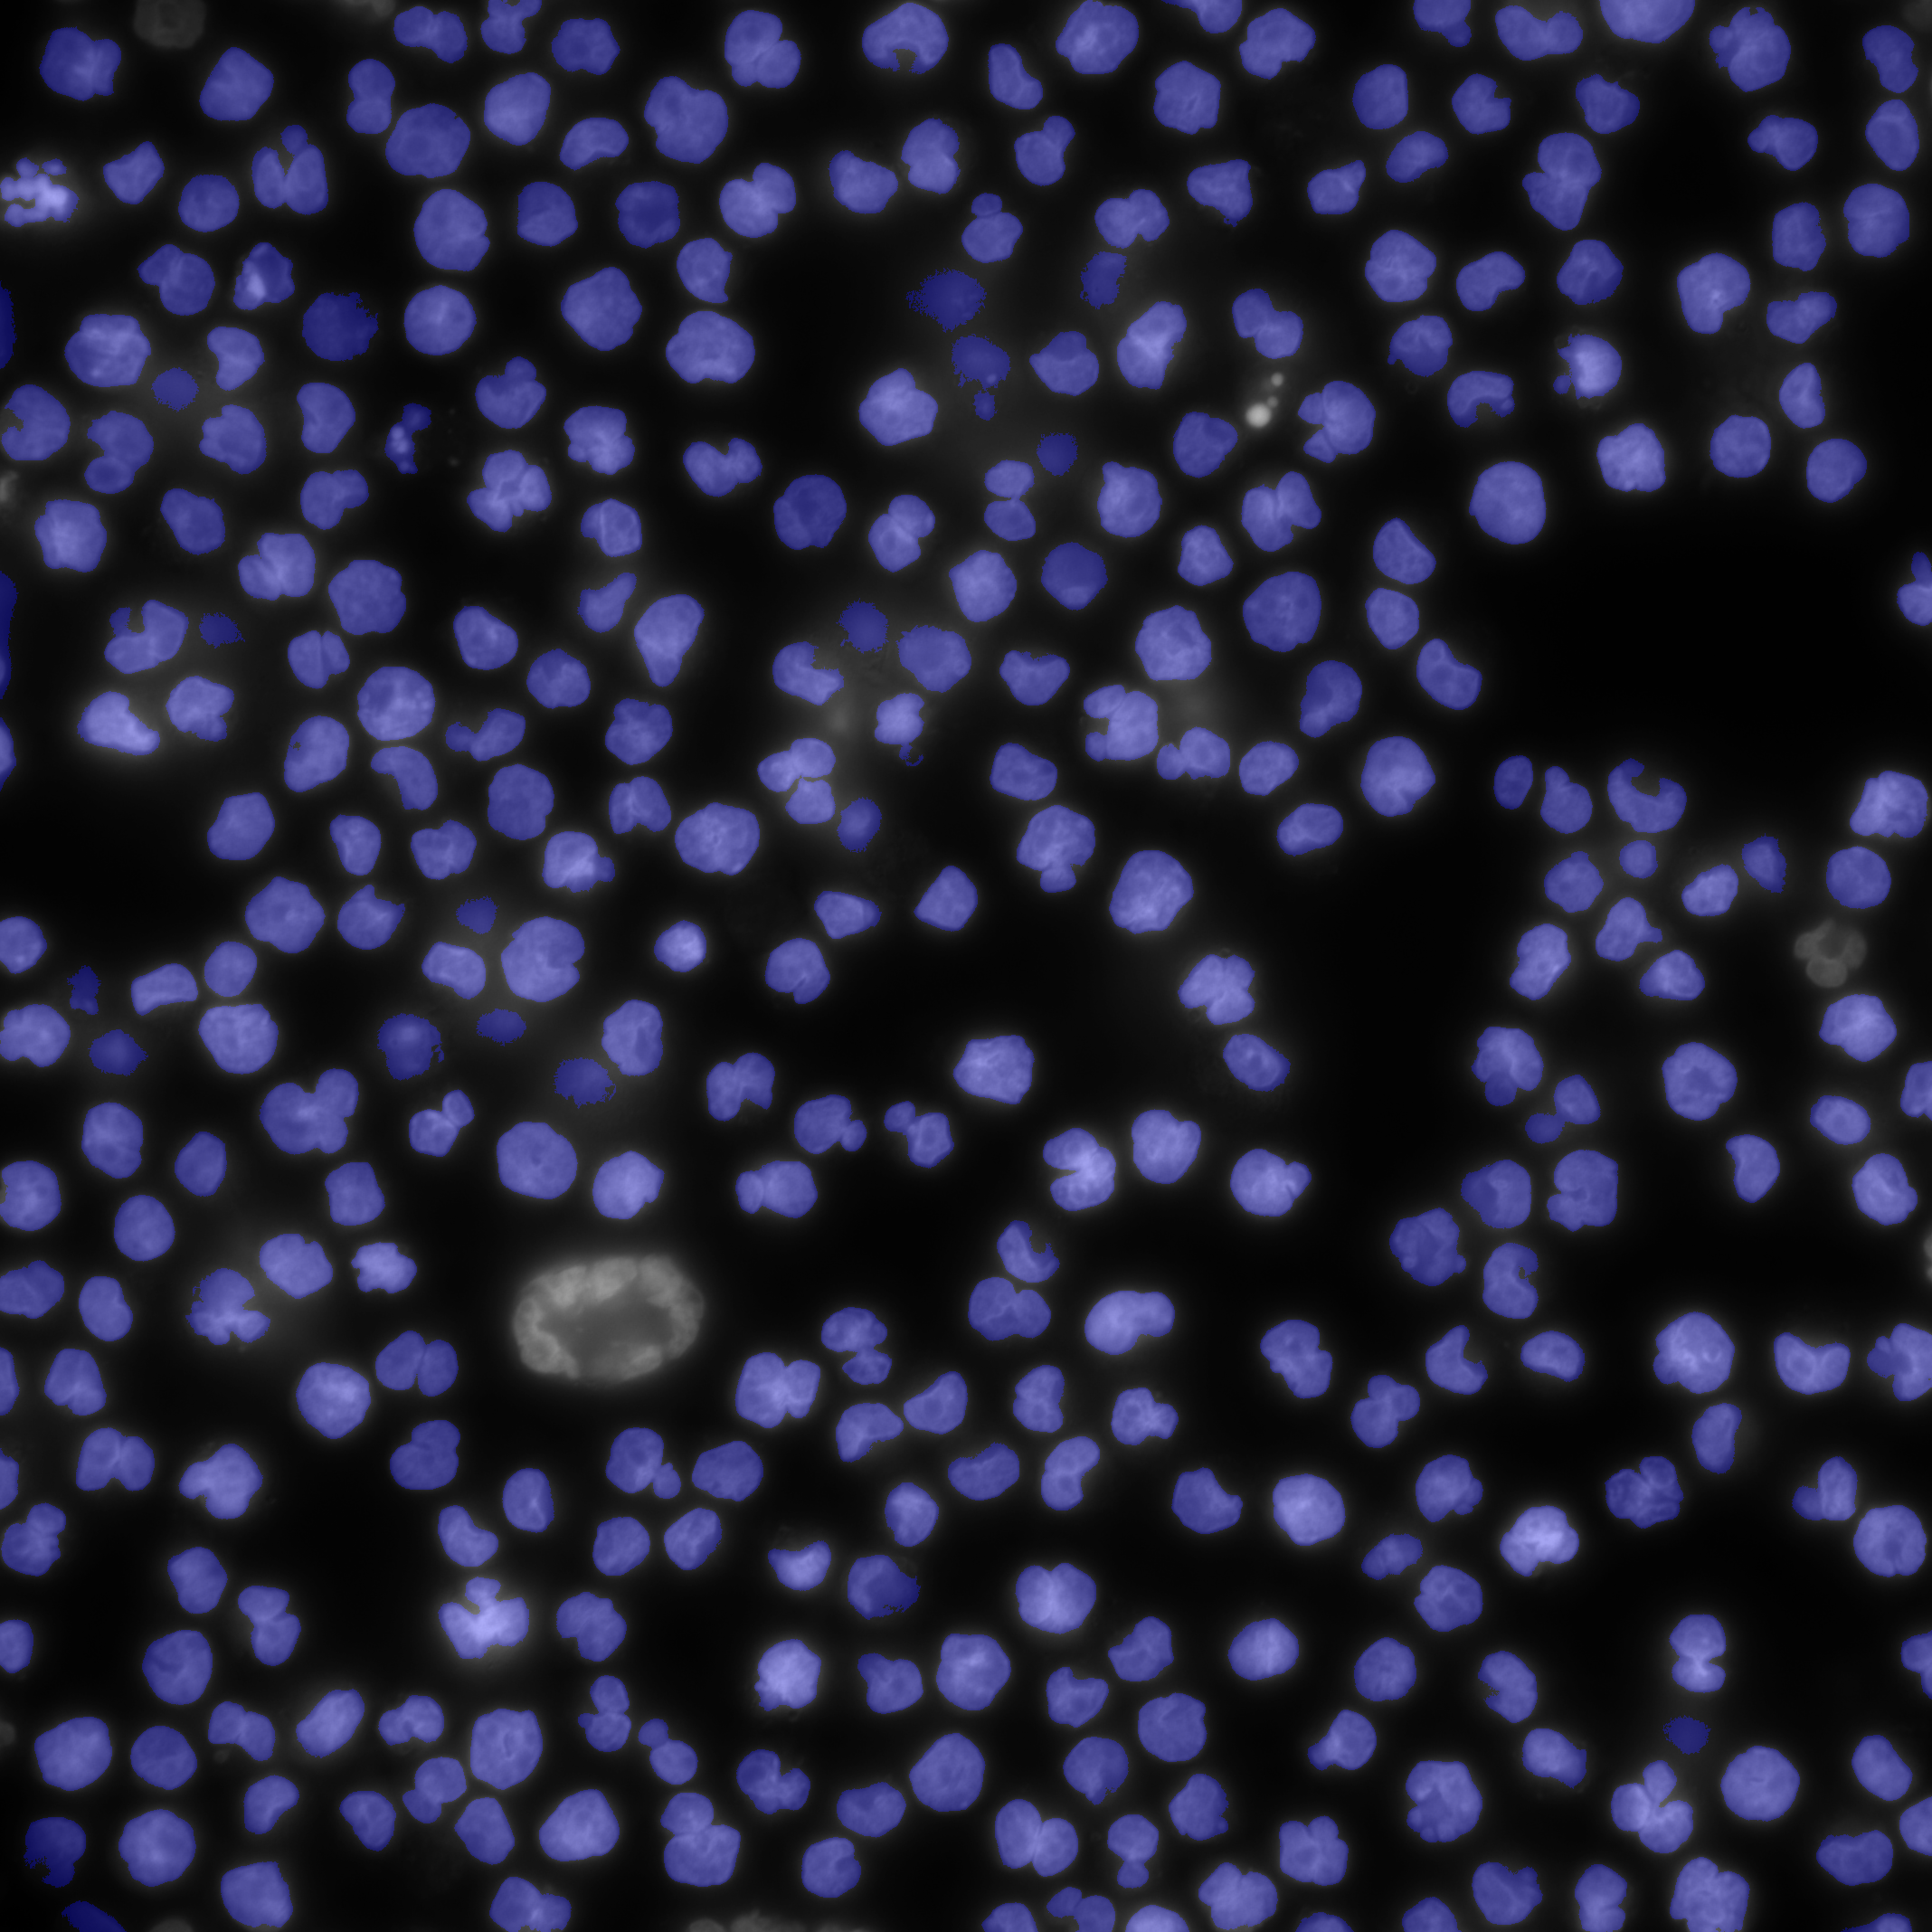
\includegraphics{bilder/difficult-lightning/normal_local.png} & 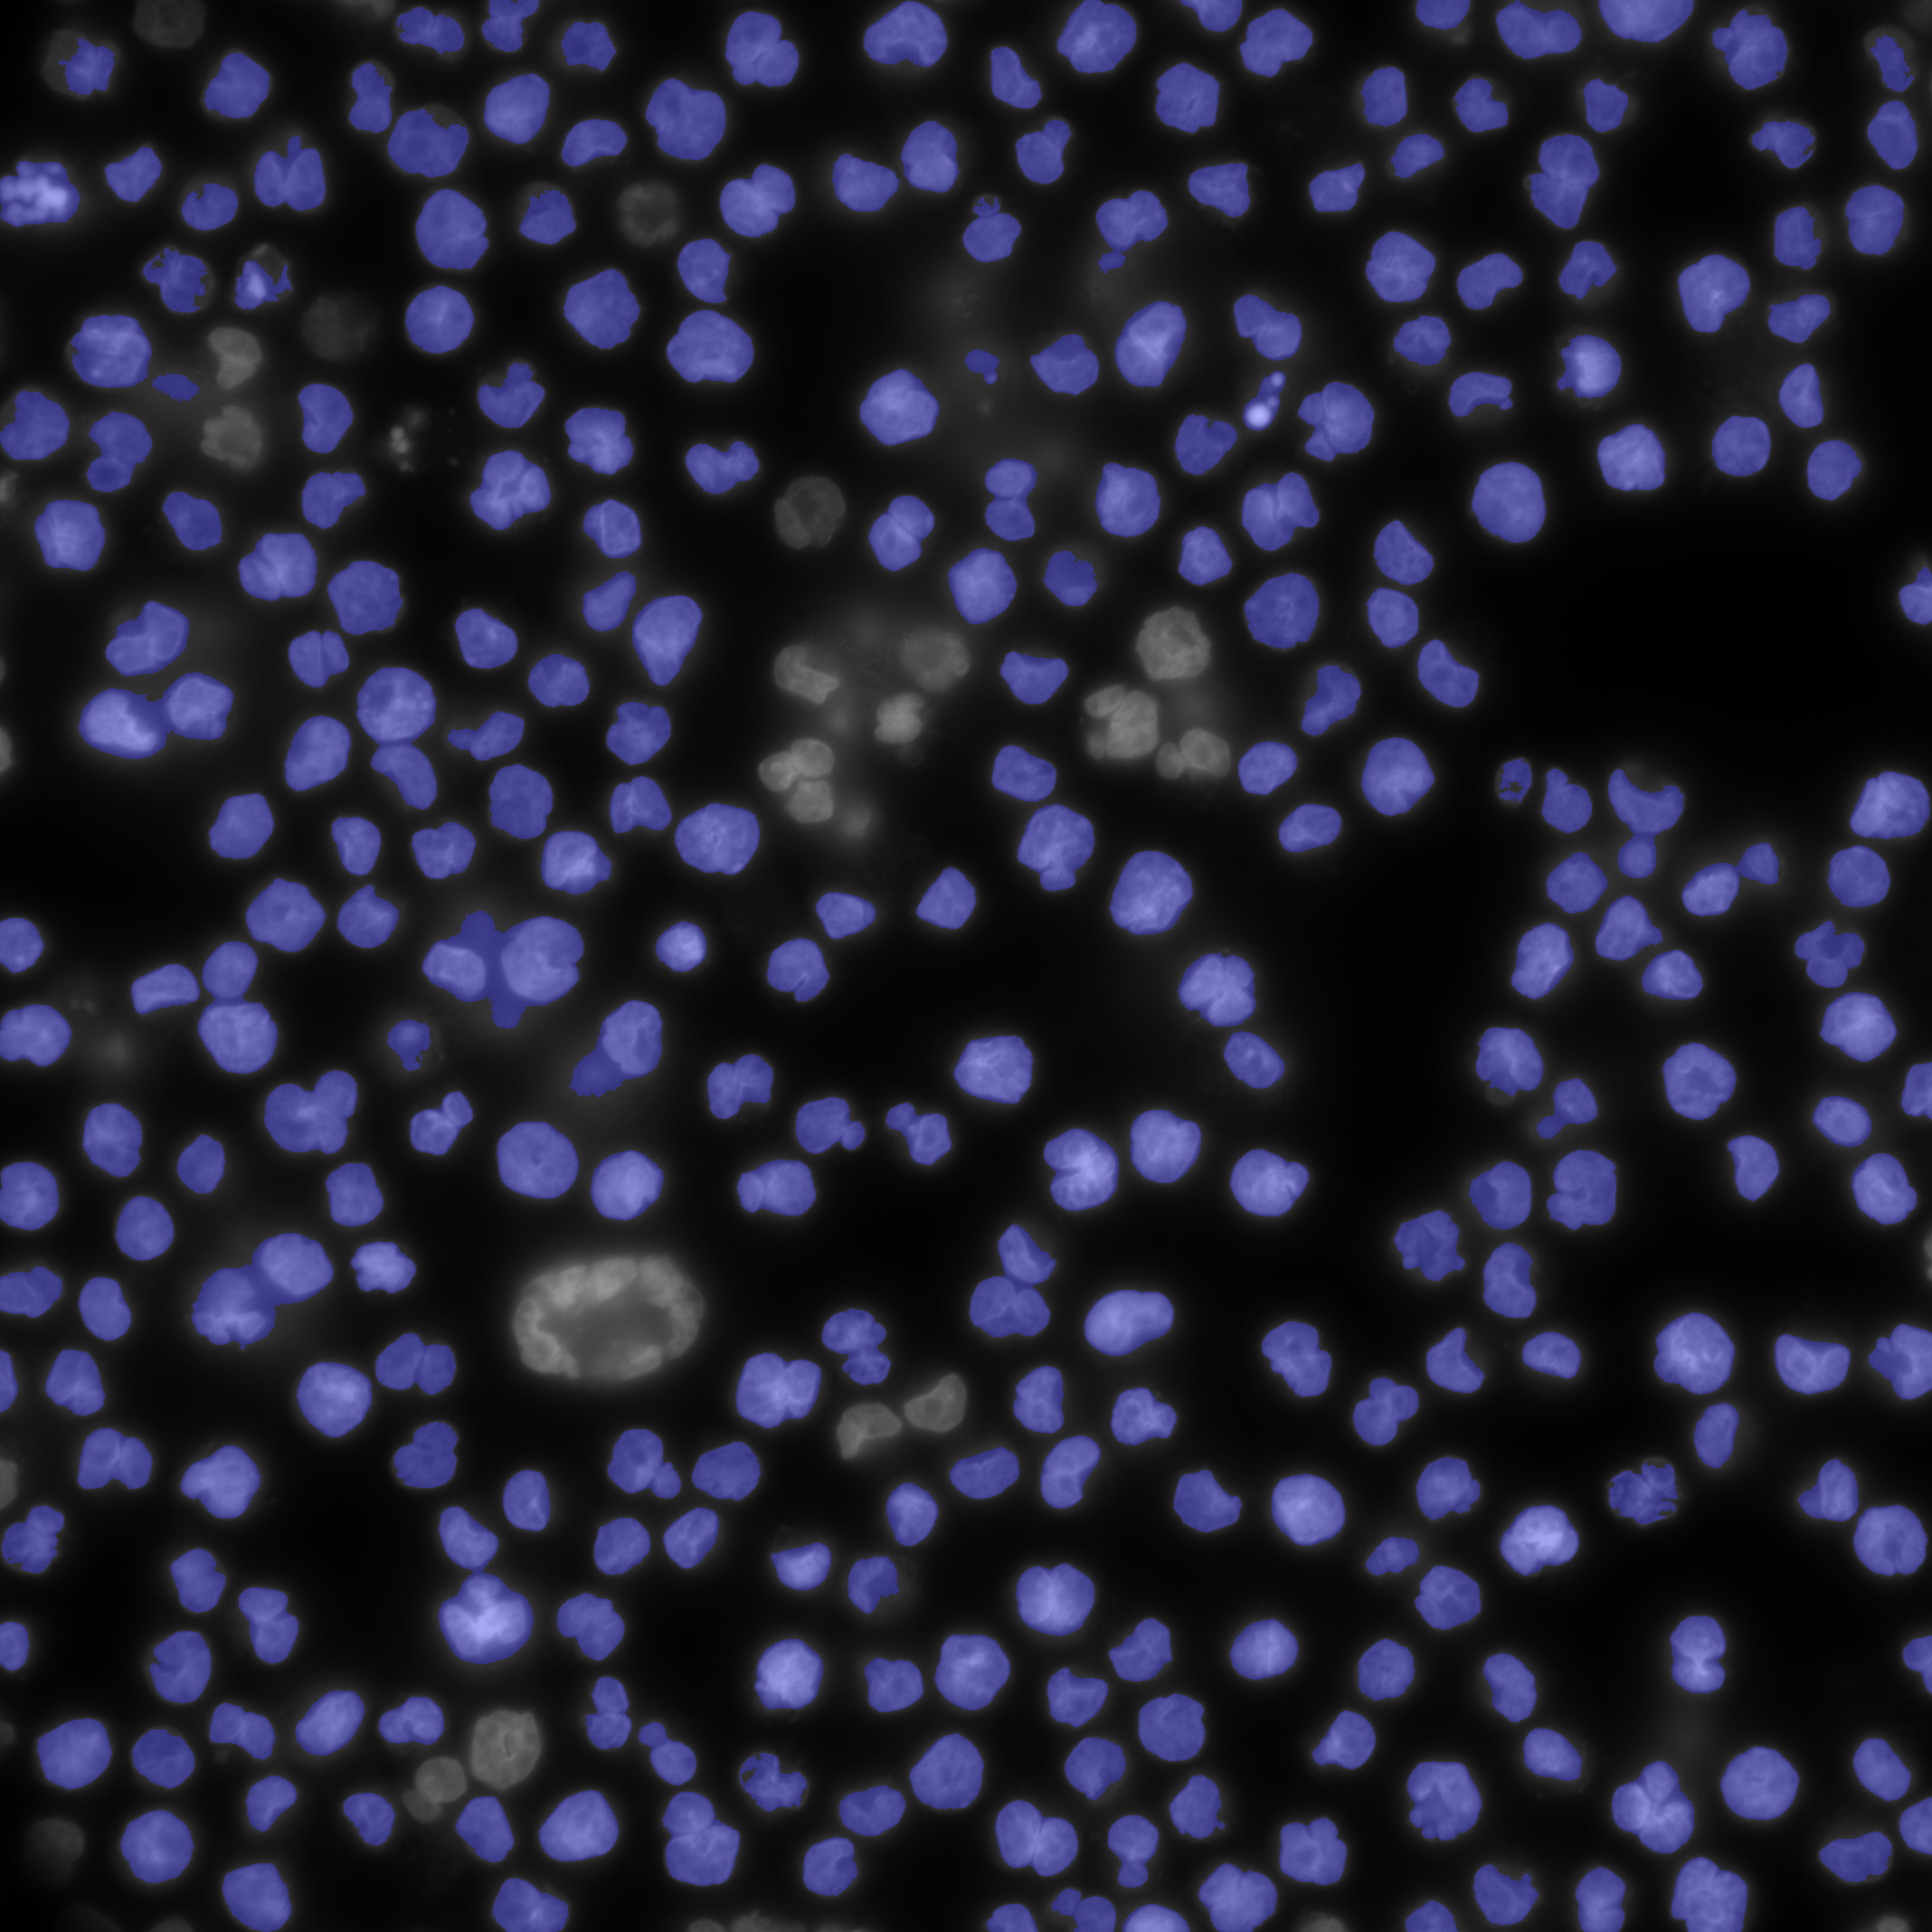
\includegraphics{bilder/difficult-lightning/normal_min.png}
        \end{tabularx}
    \caption{Local vs. Global thresholding (normal conditions)}
    \label{fig:local-vs-global-normal}
\end{figure}

According to skimage documentation, minimum thresholding works in the following way: (cite  https://doi.org/10.1111/j.1749-6632.1965.tb11715.x) it assumes that the histogram of the image is bimodal, meaning that it has two clearly defined peaks, then it iteratively smoothes the histogram using a running average of size $k=3$ (see Equation \ref{eq:SMA}) until only 2 local maximas are left. Afterwards, the lowest point between these two peaks is found and assigned to be a threshold value.

\begin{equation}
    a_k = \frac{1}{k}\sum_{i=n-k + 1}^{n}p_i
\label{eq:SMA}
\end{equation}

Then the threshold is taken as the minimum between the two local maximas.

\begin{equation}
    x_k \leq T \leq y_k
\end{equation}

TODO arrange this equation better

That is why also images which histograms have very unequal peaks or a broad and flat valley will be unsuitable for this method. (cite skimage)

\subsubsection{Overall algorithm}
With the chosen type of thresholding, the following algorithm is applied to the image to obtain the mask of nuclei:

\begin{algorithm}
    \caption{Fluorescence segmentation}\label{alg:global-thresholding}
    \begin{algorithmic}
    \item 1. Normalize image.
    \item 2. Apply chosen thresholding and get a threshold $T$ or a set of local thresholds \{$T_i$\} and create an initial mask: $1$ if $x_i > T$ or $0$ otherwise.  
    \item 3. Apply \textit{fill\_holes} transformation to the initial mask in order to get rid of unneeded details insides the nuclei.
    \item 4. Run \textit{findContours} from opencv in order to obtain separate regions and filter them based on the following criteria: filter out too big regions (measure the biggest possible nuclei manually), too small regions (measured manually as well), regions that have a shape that it not very similar to convex circular type of nuclei. The last filter is done by checking the ratio of the area of the region to the area of the convex hull of the region. 
    \end{algorithmic}
\end{algorithm}    

Subsequent steps of such algorithm are presented in the Figure \ref{fig:segmentation-nuclei-steps}

\begin{figure}[H]
    \centering
    \setkeys{Gin}{width=\linewidth}
    \centering
        \begin{tabularx}{\textwidth}{YYYY}
            \textbf{Normalized input} &
            \textbf{Local threshold} &
            \textbf{Filled holes} &
            \textbf{Filtered regions} \\
            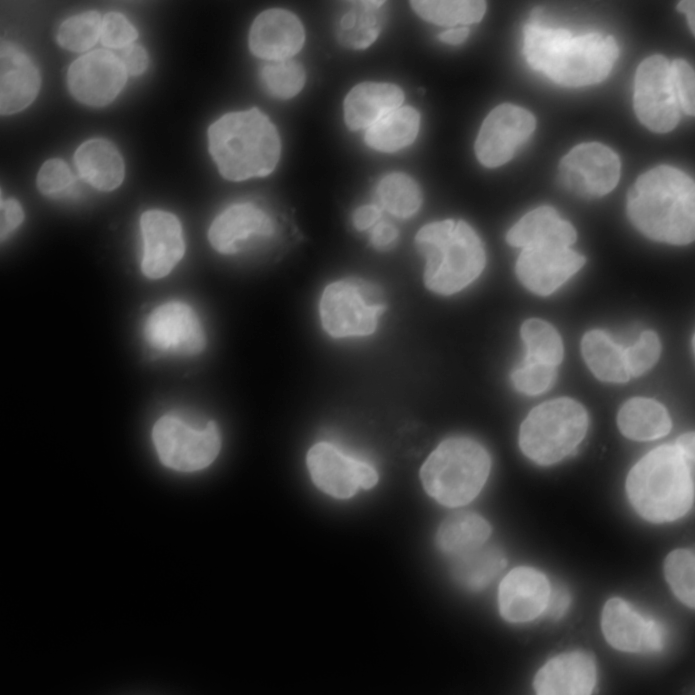
\includegraphics{bilder/segmentation/nuclei-mask/normalized.png} & 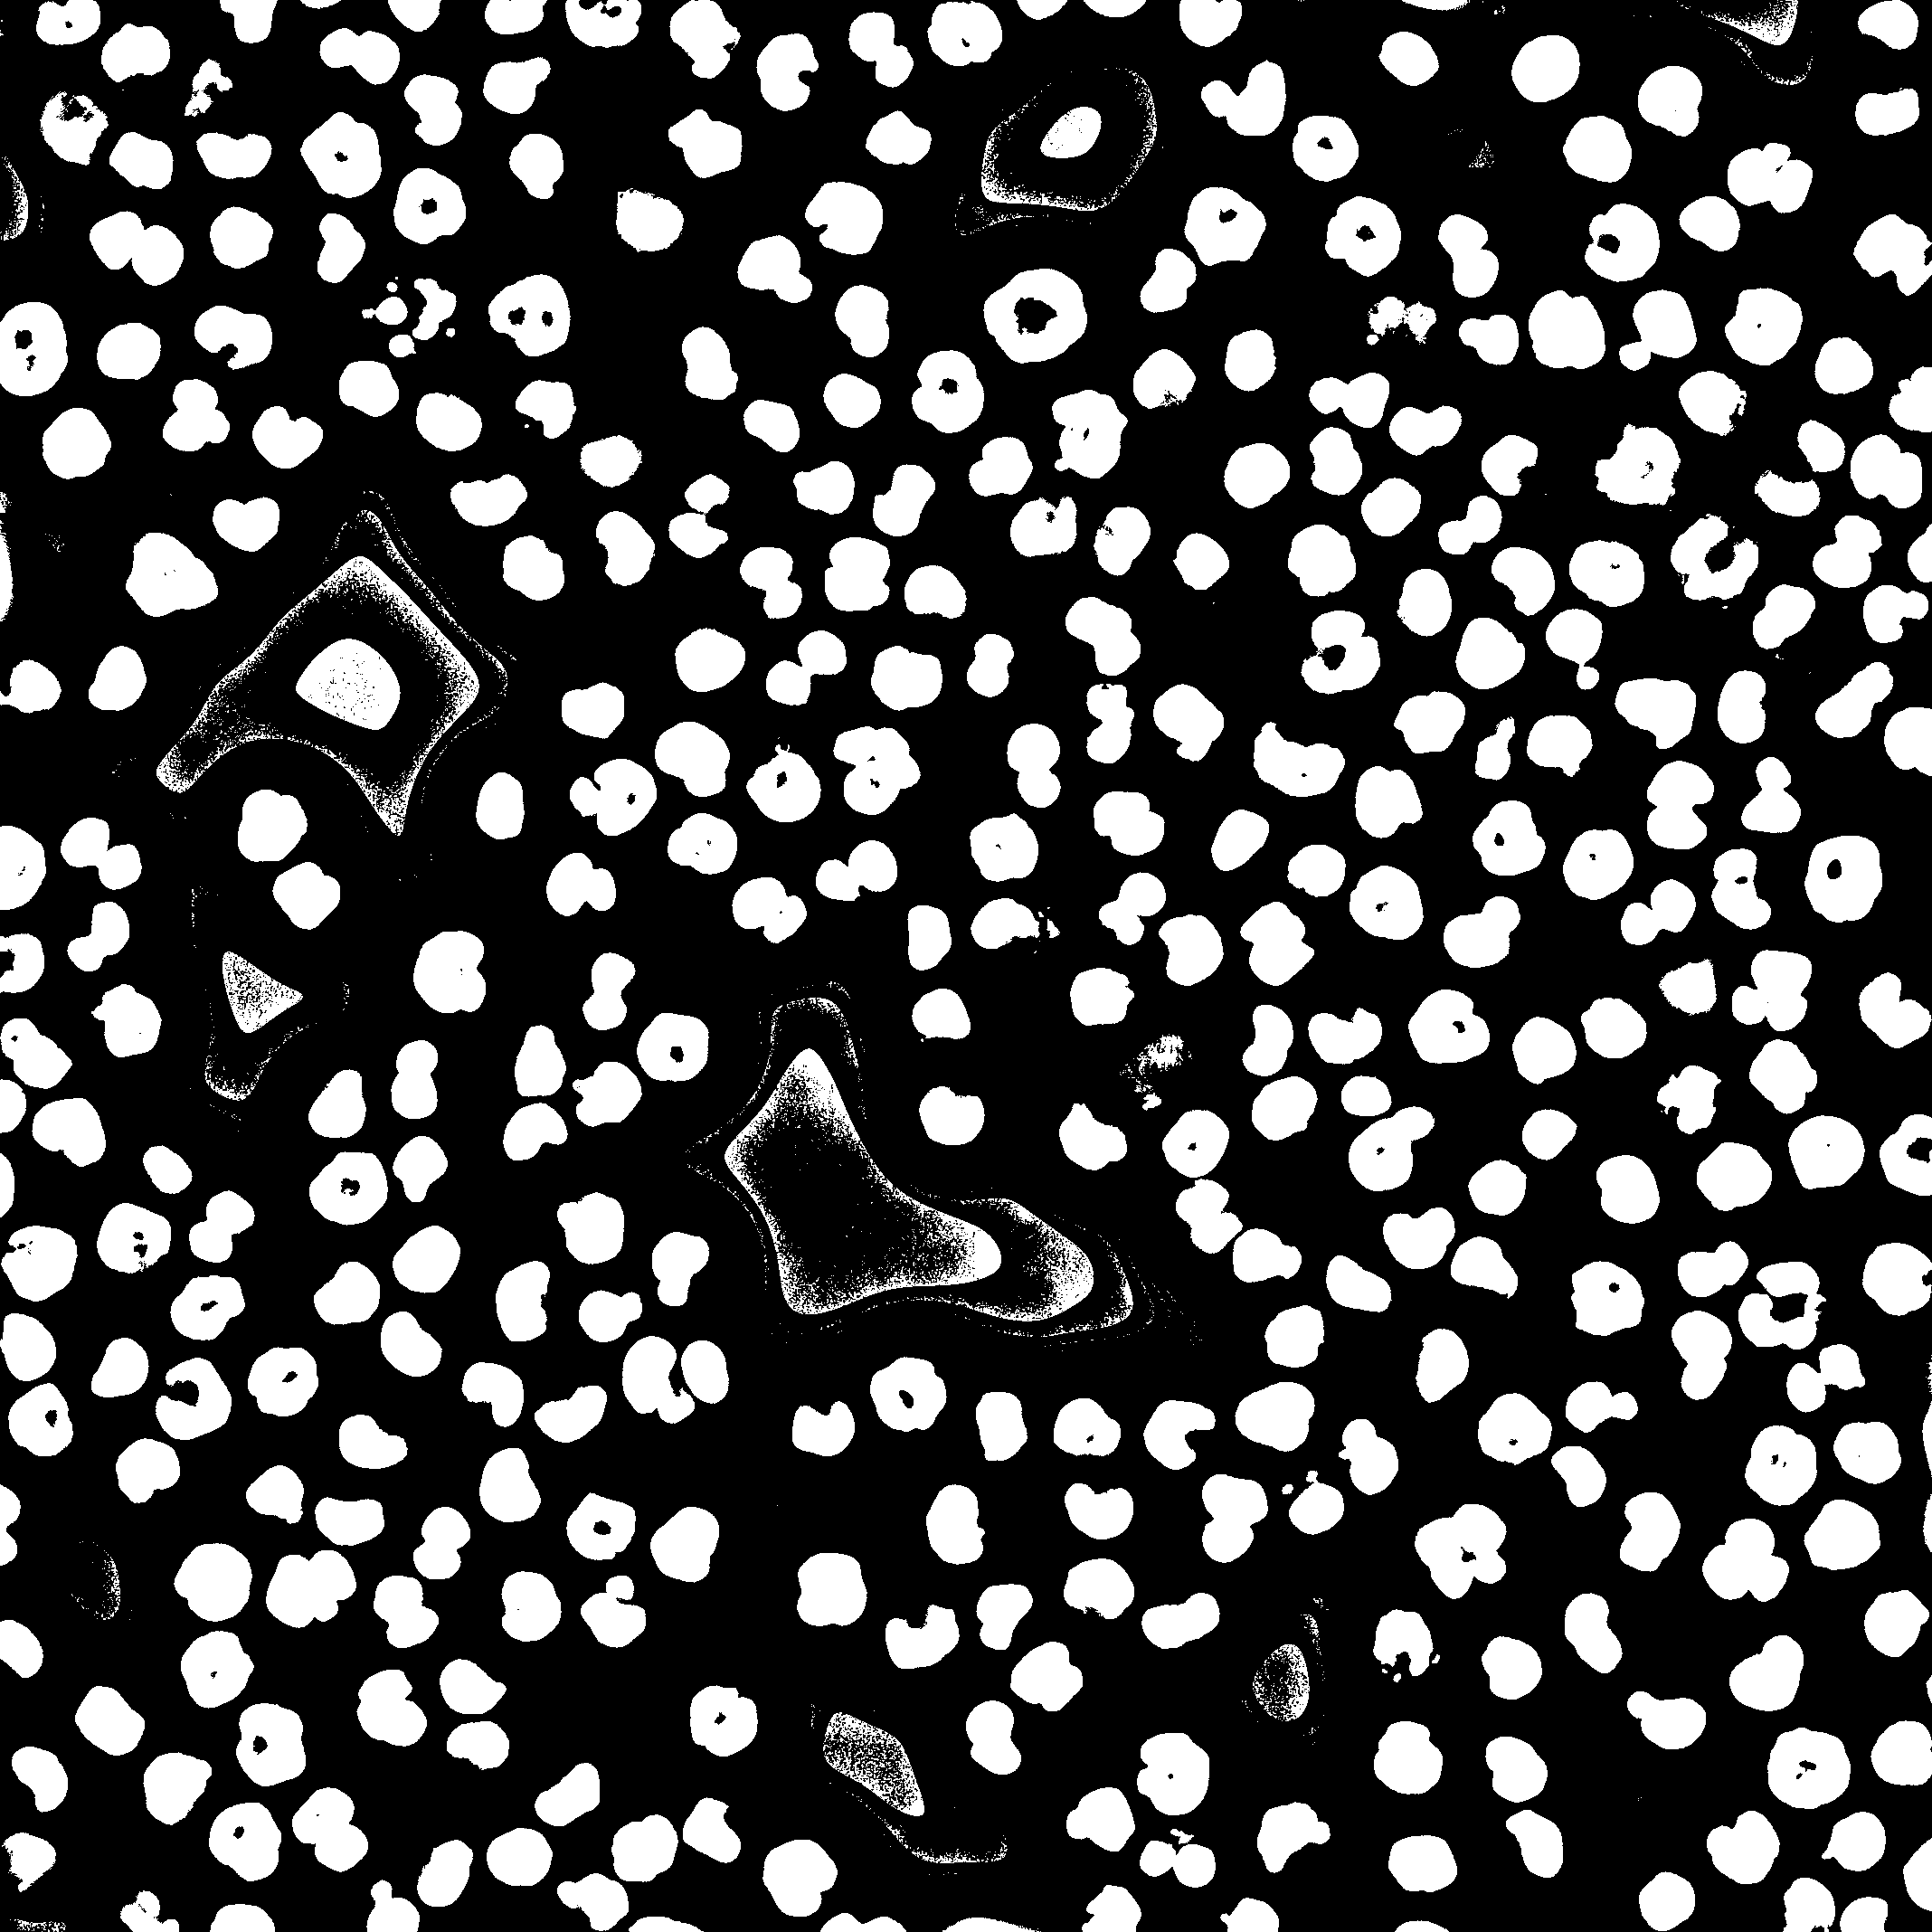
\includegraphics{bilder/segmentation/nuclei-mask/binary_local.png} &
            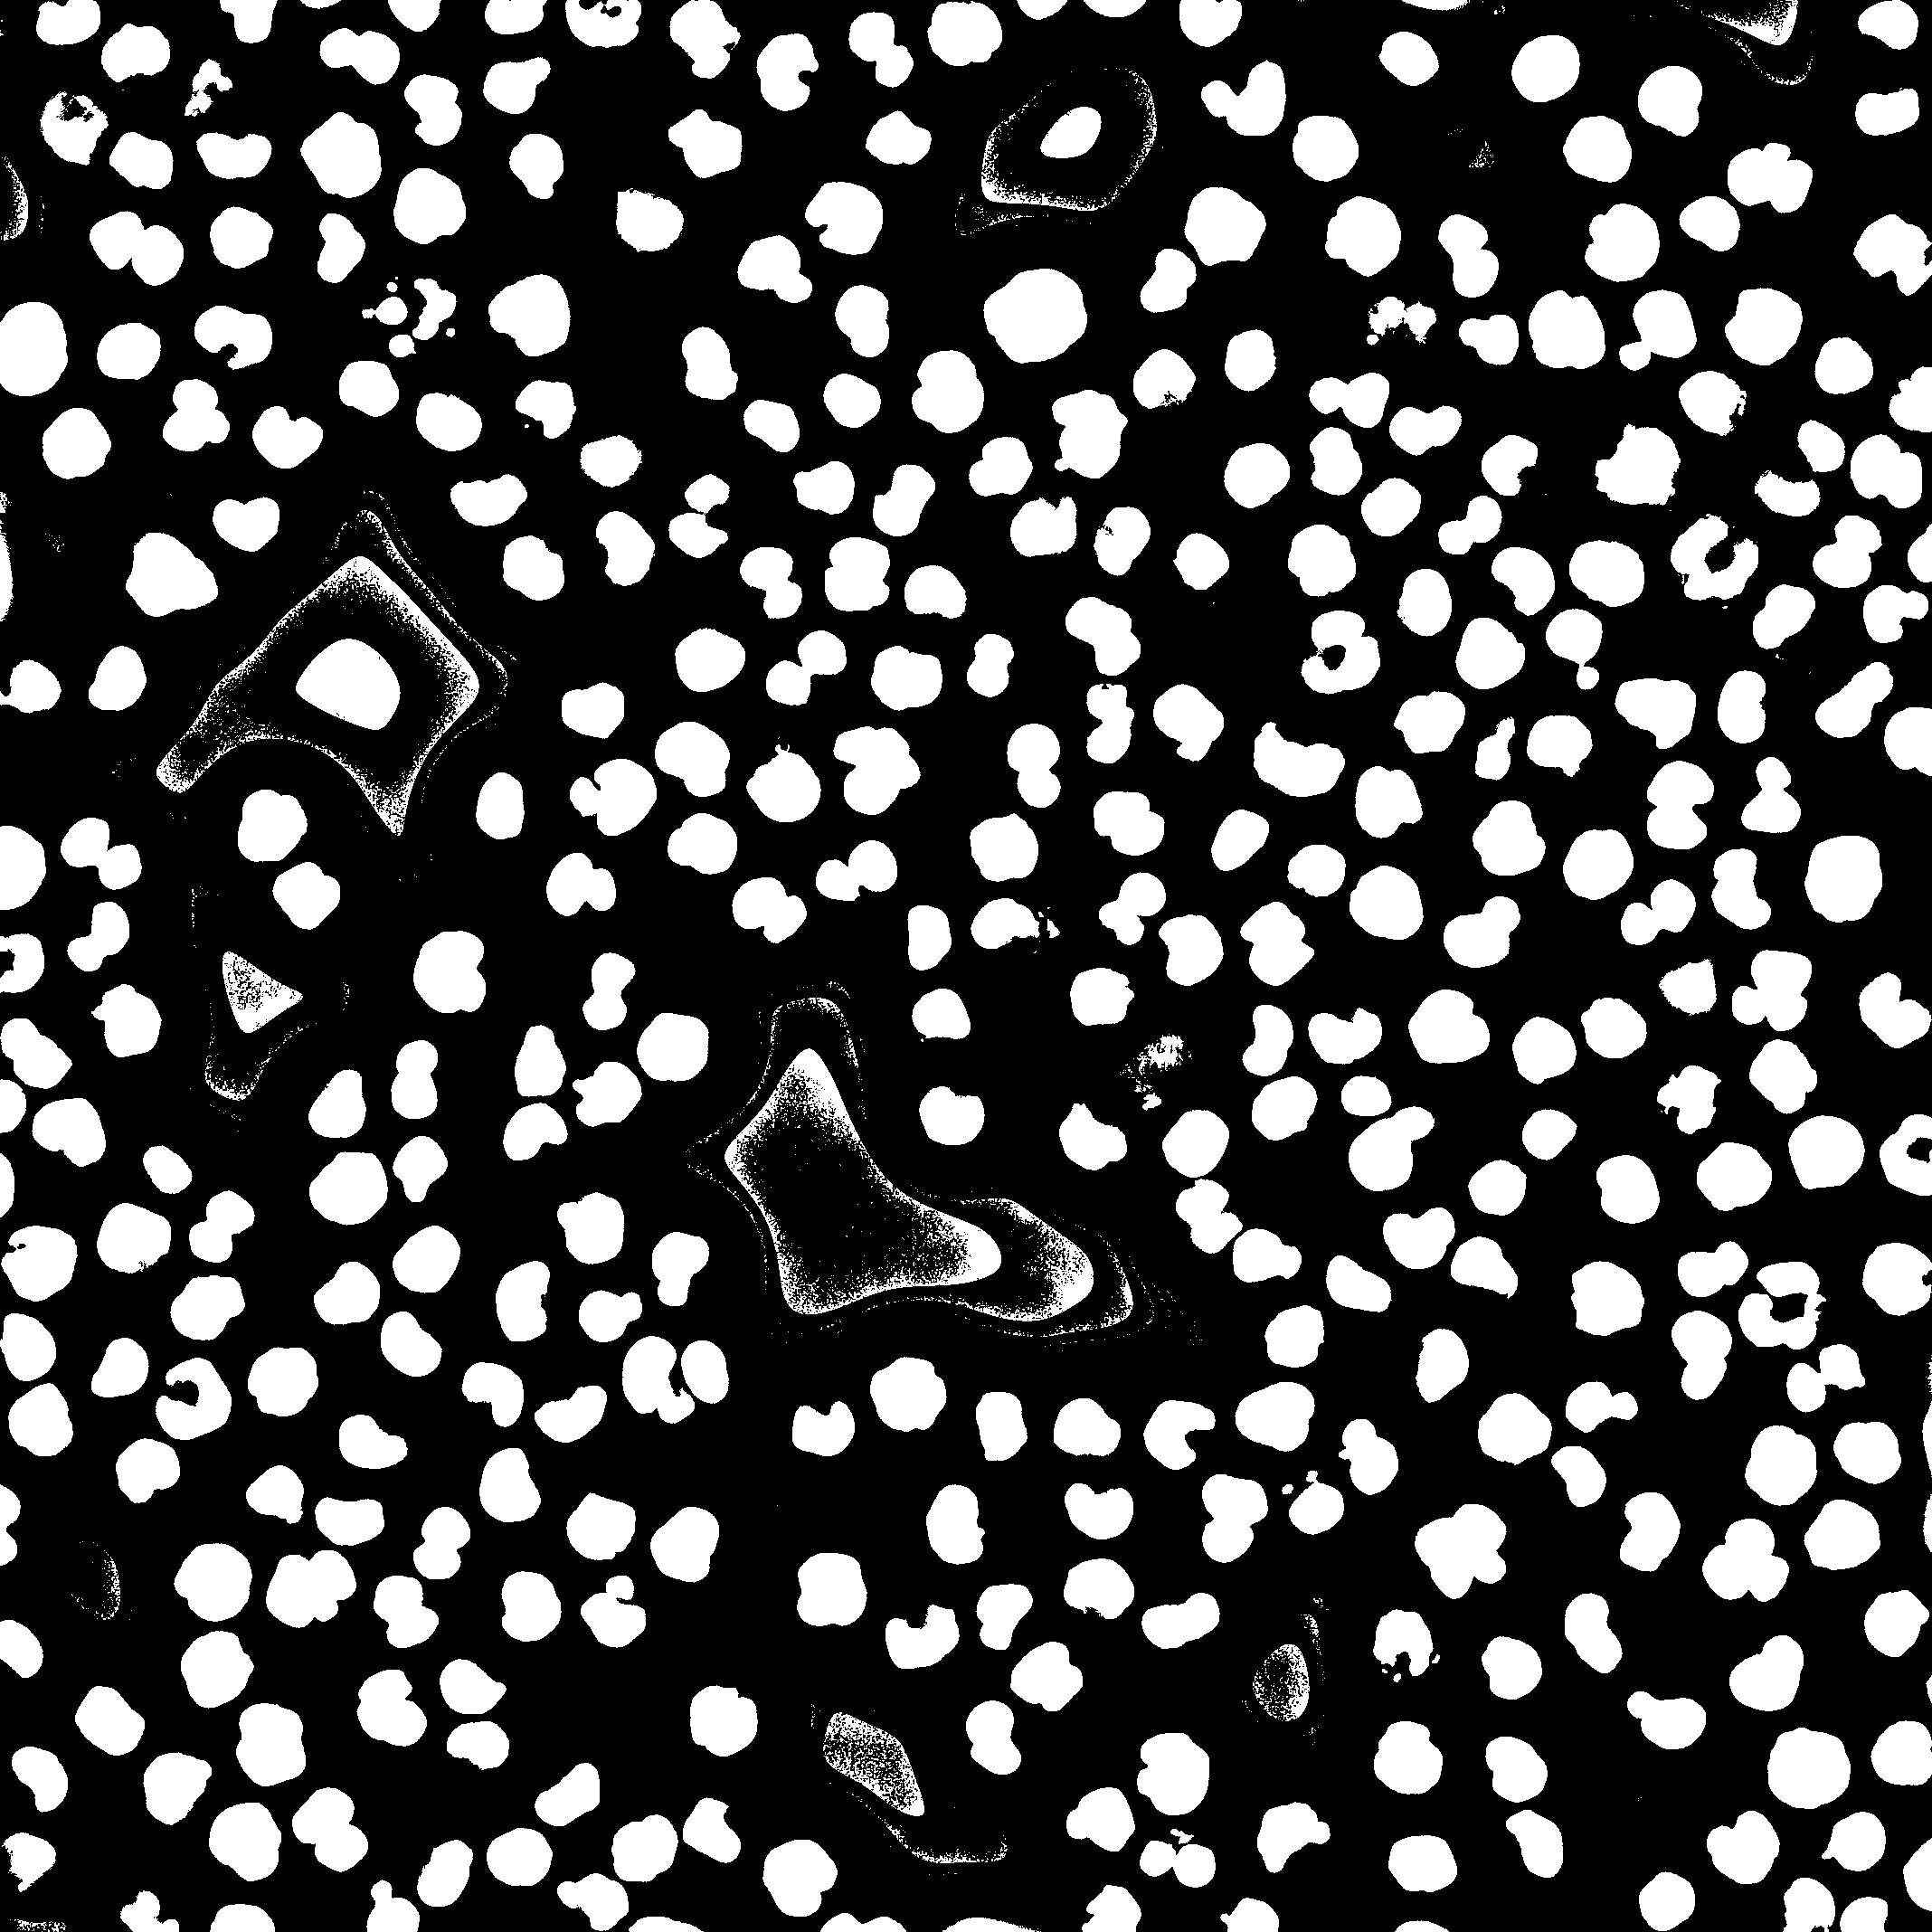
\includegraphics{bilder/segmentation/nuclei-mask/filled_holes.png} & 
            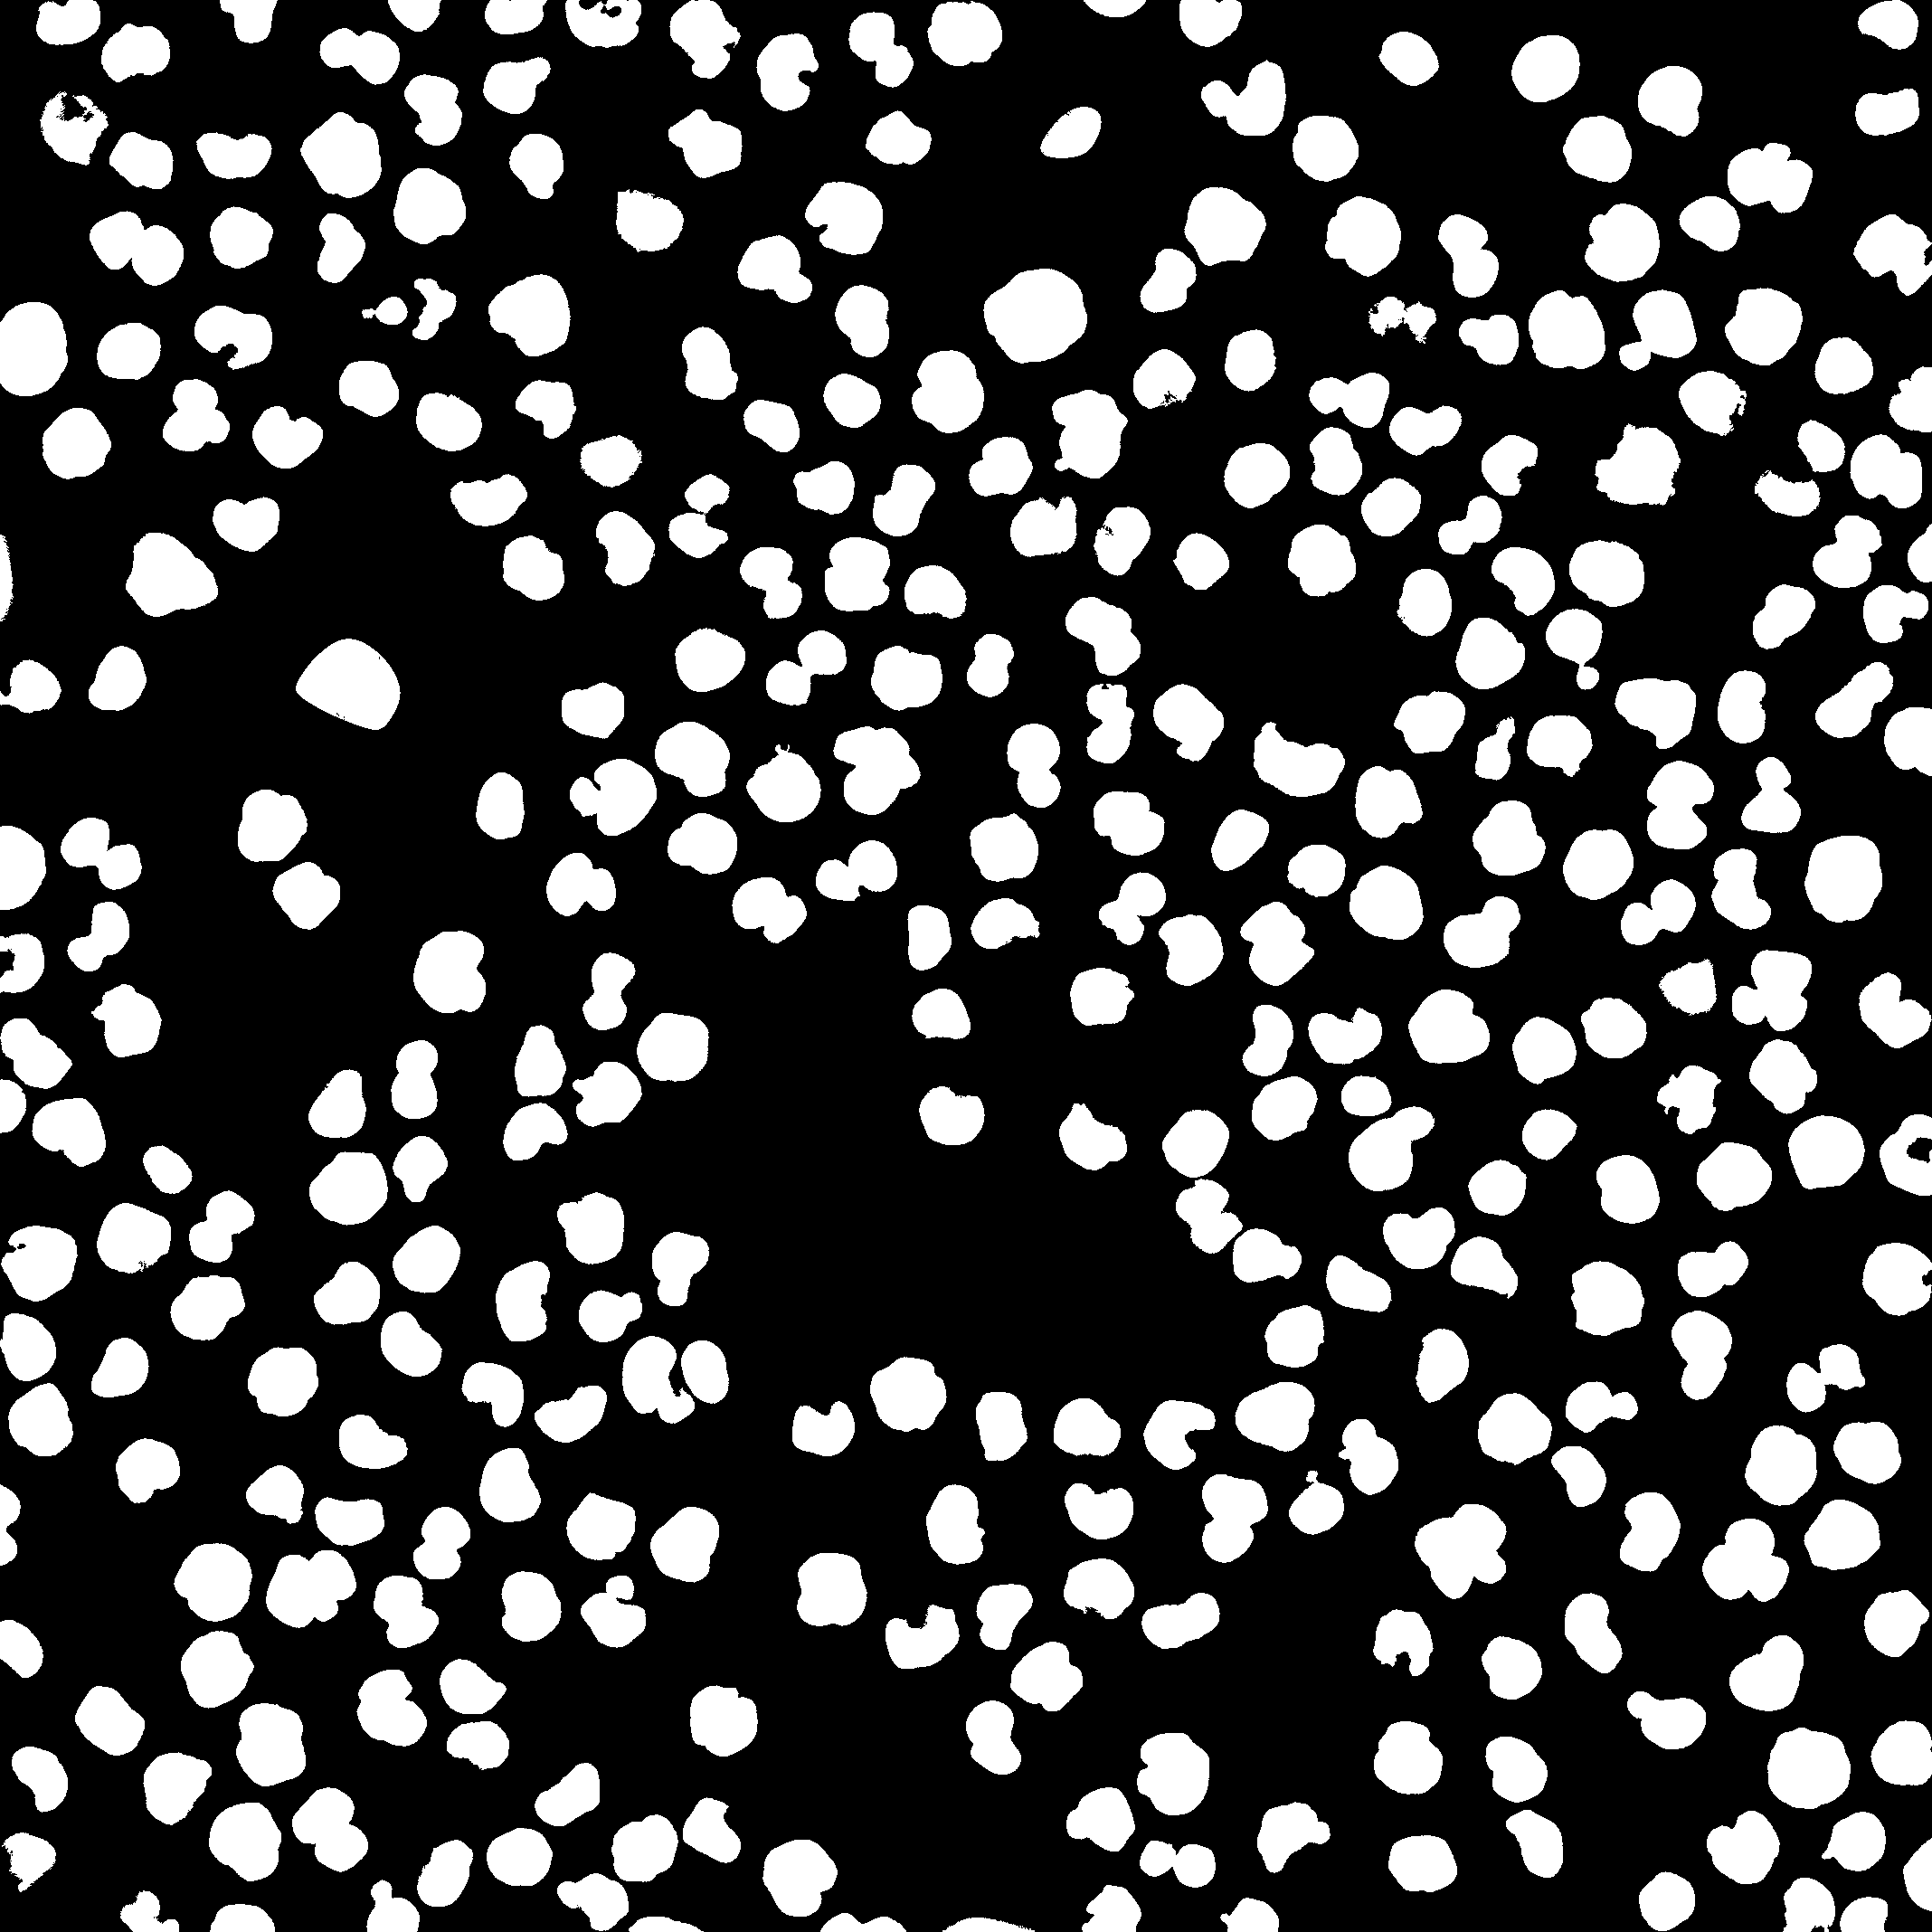
\includegraphics{bilder/segmentation/nuclei-mask/mask.png}
        \end{tabularx}
    \caption{Fluorescence segmentation}
    \label{fig:segmentation-nuclei-steps}
\end{figure}


\subsection{ER-segmentation}
Endoplasmic reticulum or ER is another cell organelle. It is a continuos membrane system that forms a series of flattened sacs within the cell. It has many important functions such as synthesis, folding, modification, and transport of proteins. (Rogers, Kara. "endoplasmic reticulum". Encyclopedia Britannica, 11 Nov. 2020, https://www.britannica.com/science/endoplasmic-reticulum. Accessed 16 May 2022.) Therefore detecting ER within the cell and its quaility and its further analysis can give insights on the protein production of the cell. For example the proximity of the ER to the nucleus allows it to control the protein production. For example, when the protein os misfolded or incorrectly folded it will accumulate in the ER lumen and will be a signal to activate misfolded protein response. 

\begin{figure}[H]
    \centering
    \setkeys{Gin}{width=\linewidth}
    \centering
        \begin{tabularx}{\textwidth}{YYYY}
            \textbf{Ground truth} &
            \textbf{Prediction} &
            \textbf{Prediction + nuclei} \\
            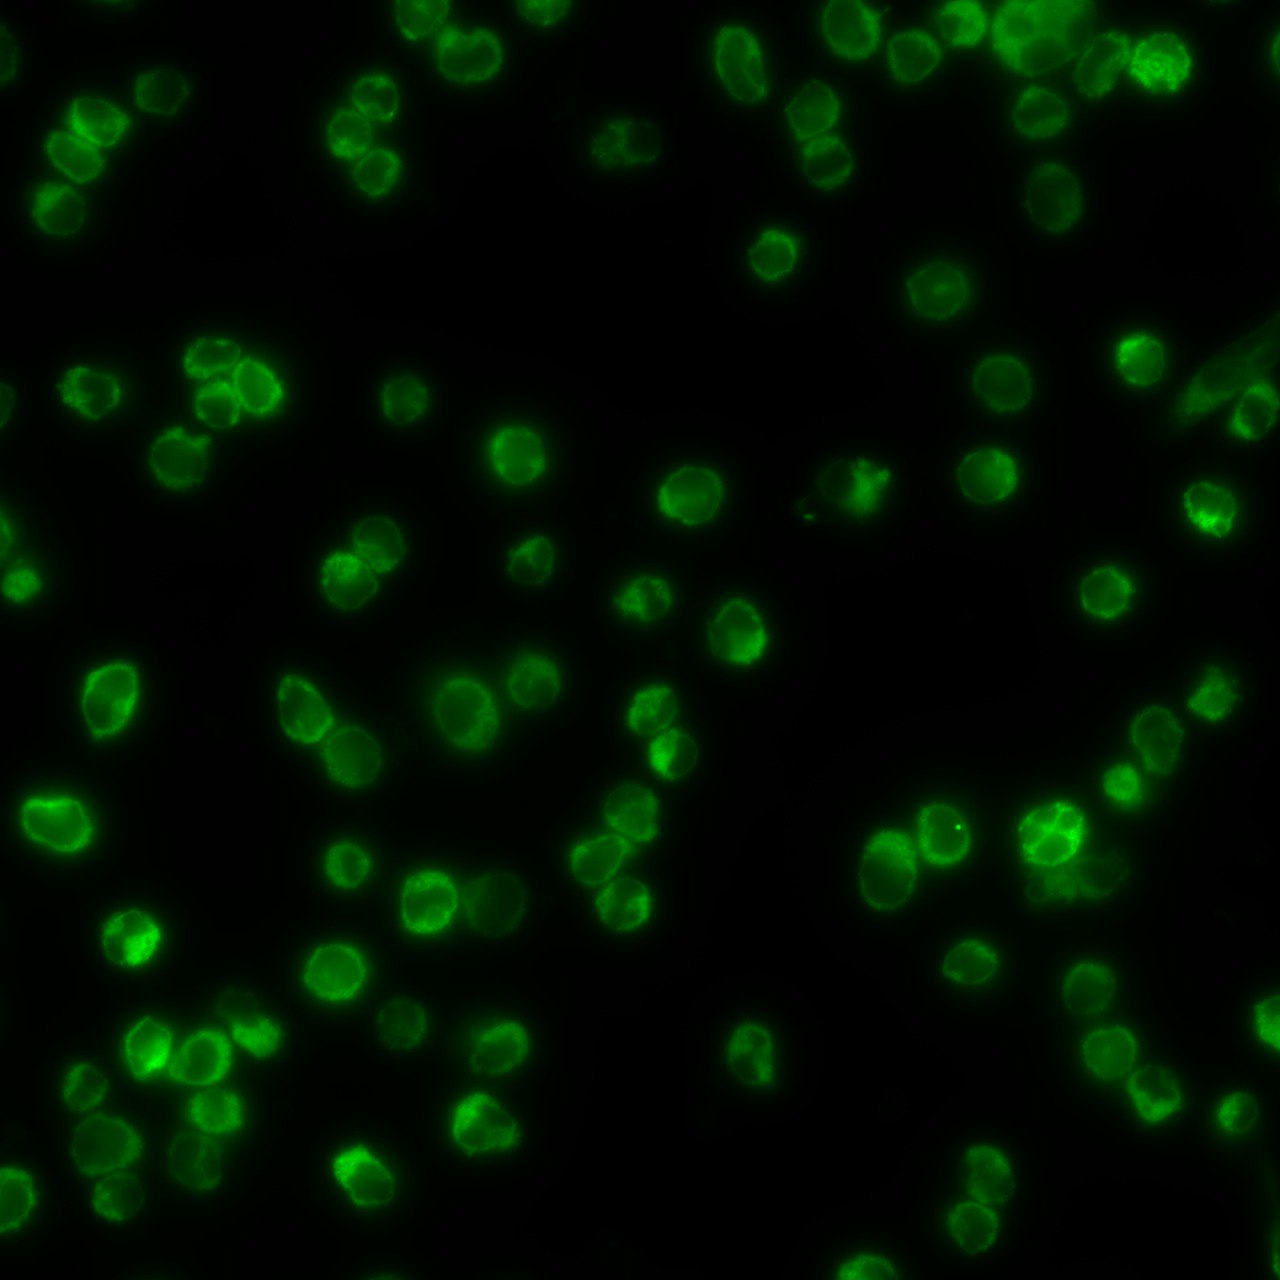
\includegraphics{bilder/ER/gt.jpg} & 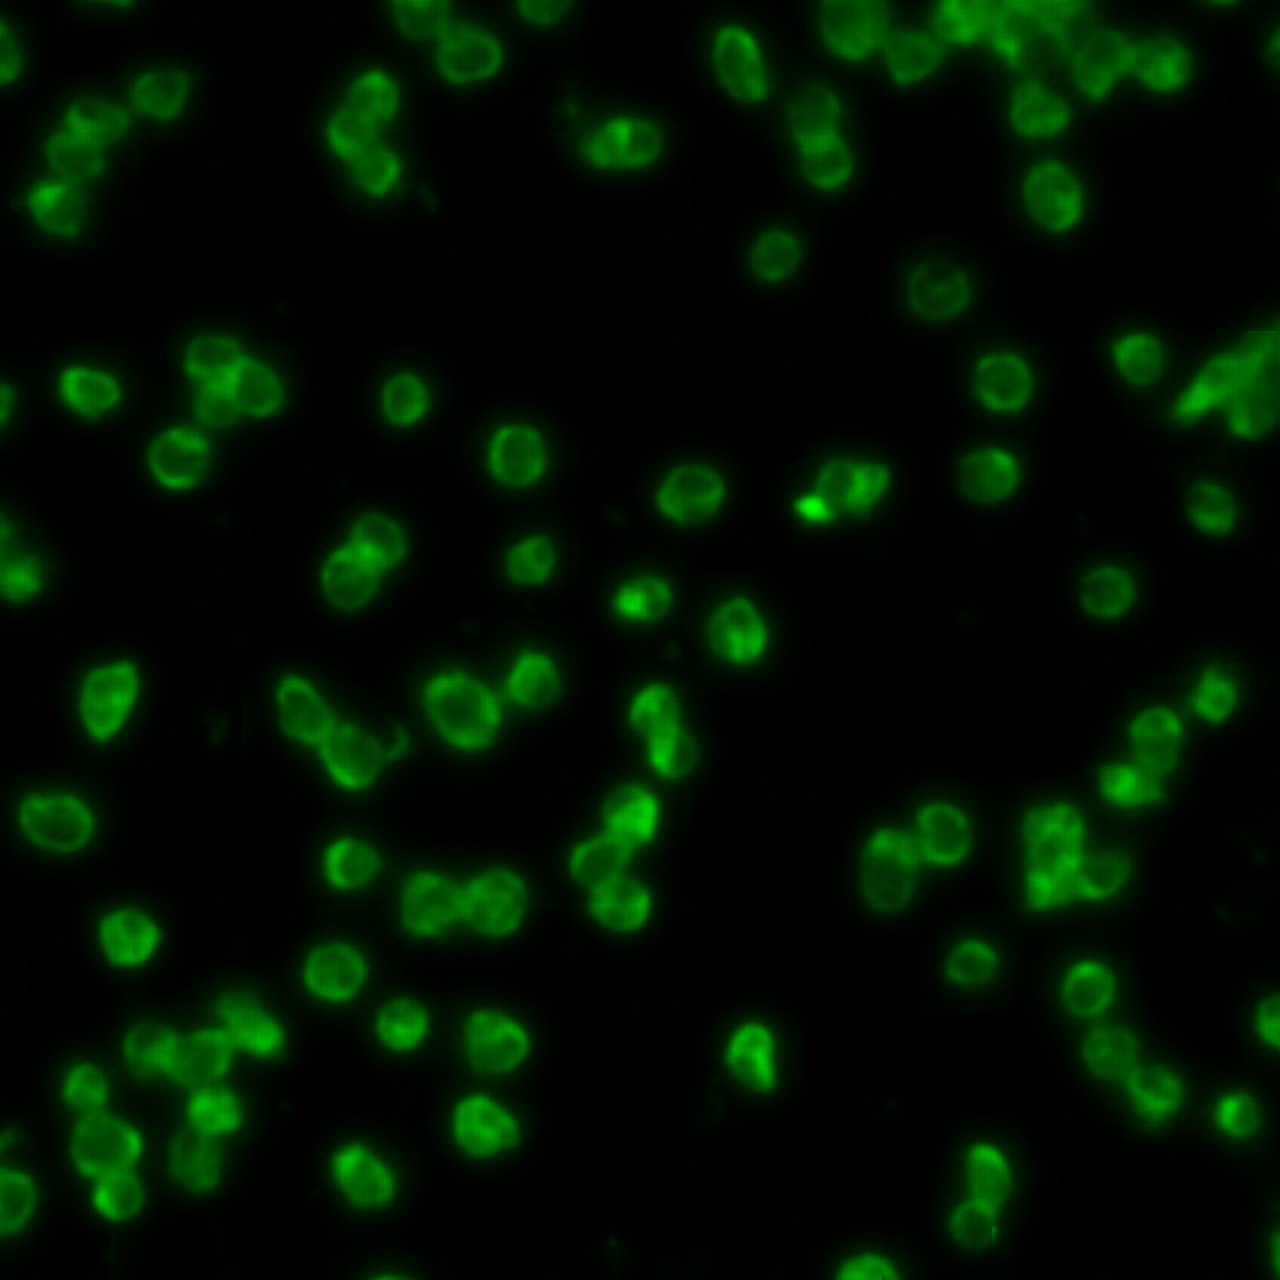
\includegraphics{bilder/ER/er.jpg} &
            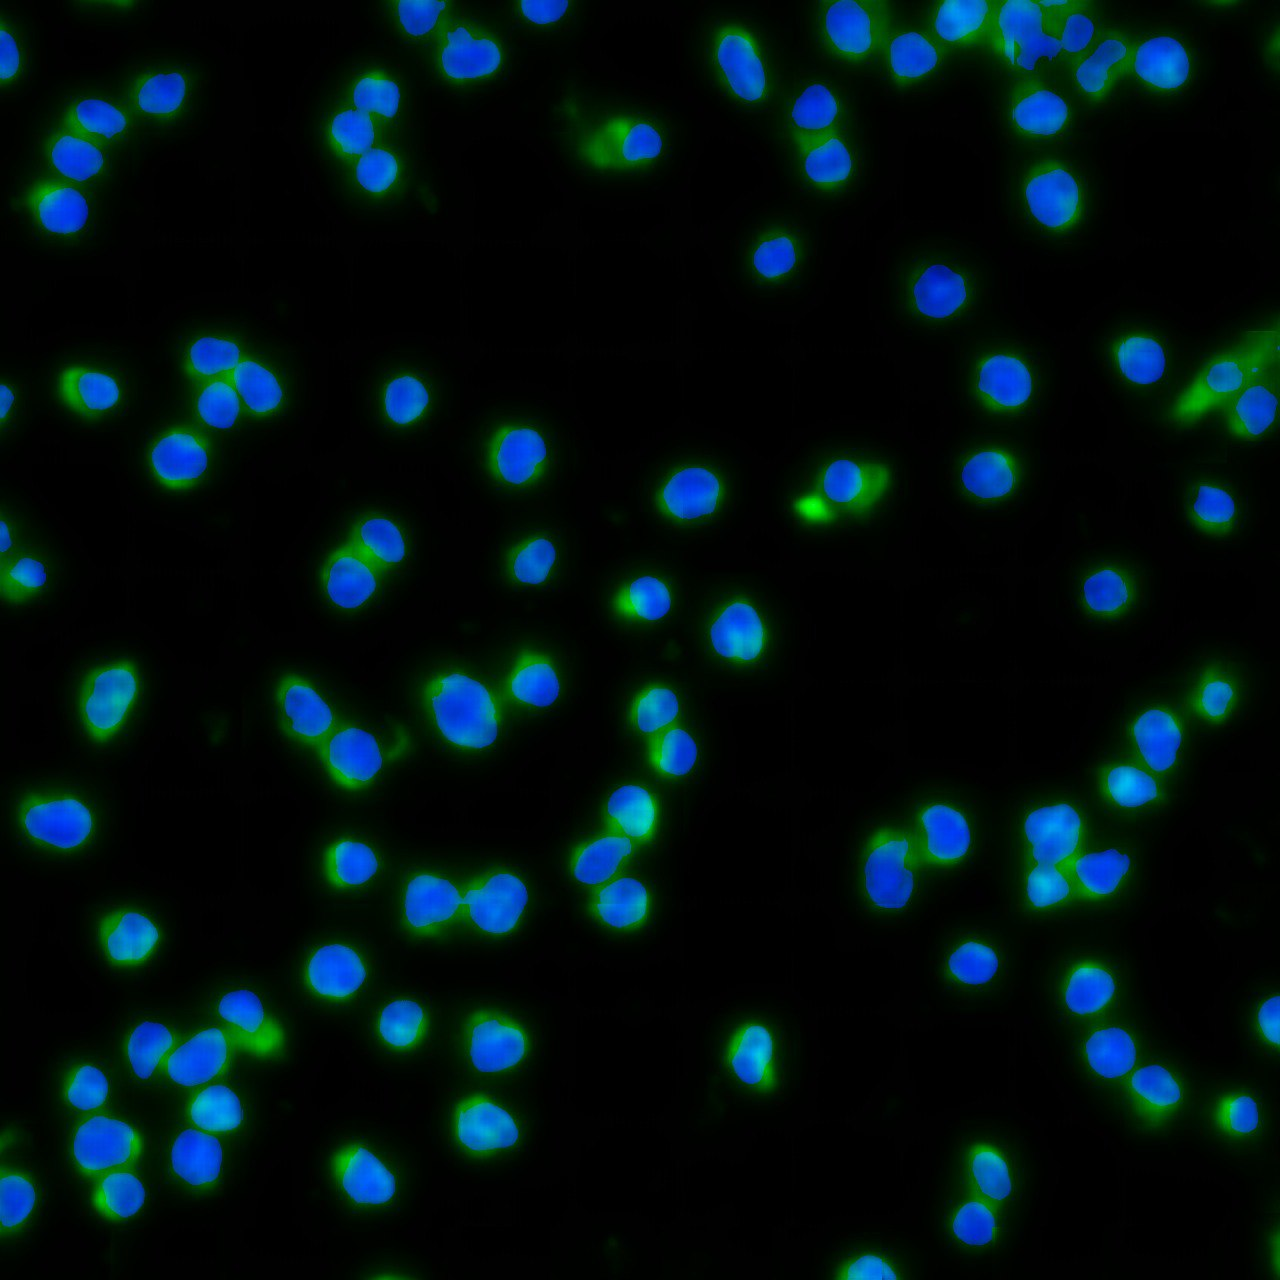
\includegraphics{bilder/ER/gt_nuclei.jpg}
        \end{tabularx}
    \caption{ER prediction}
    \label{fig:er-prediction}
\end{figure}

For staining this organelle Fluorescein isothiocyanate (FITC) method was used. The process of ER fluorescence segmentation is somewhat different to nuclei segmentation. These fluorescence staining has a stronger "shining" around the ER itself and therefore a simple background removal would be helpful to reduce it. Another big reason to use this approach hides in the escaping of the background noise recognized as a signal by the further local thresholding algorithm as in Figure \ref{fig:segmentation-nuclei-steps} c. Such regions from the background noise cannot be filtered out that easily for ER-fluorescence. Ther reason is the following: the main criteria for filtering such regions in nuclei fluorescence imaging was the shape of the region. All nuclei are almost round and convex, while background noise might be not convex at all. However in FITC imaging some of the cells are located so close one to another that they may form a long non-convex object that would be filtered out based on previous criteria. Therefore removing the background noise if an improvement for pre-processing of images on which the local thresholding would be performed.

In order to do that one can first apply a rough over-predictive global thresholding over the fluorescence image, that will cover a true signal fully and ignore the background noise. Mean thresholding algorithm was chosen for this as it perfectly does the over prediction for these images (see Figure TODO ref). The mask created with the mean thresholding approach is used to zero out all the pixels that are not covered in the mask. Only after that the local thresholding is applied (in comparison to nuclei where one can apply local thresholding directly) with the TODO 181 (Fugure TODO). Then  algorithm covers all the holes in the middle on the cells in fluorescence that might have appeared during the thresholding. Morphological opening (see Section TODO) and Gaussian Blur with the squared kernel 3x3 are applied. Connected components are detected afterwards and filtered based on the limit of the area they occupy, this filters out mostly very small components from the mask which might be produced by the left out background noise. The whole algorithm overview you can find here:


\begin{algorithm}
    \caption{Fluorescence segmentation}\label{alg:global-thresholding}
    \begin{algorithmic}
    \item 1. Normalize image
    \item 2. Apply global \textit{threshold\_mean} to receive initial mask.
    \item 3. Zero out pixels outside the mask
    \item 4. Apply local thresholding.  
    \item 5. Apply \textit{fill\_holes} transformation.
    \item 6. Morphological opening from opencv and Gaussian blur.
    \item 7. Run \textit{findContours} from opencv in order to obtain separate regions and filter out too small regions.
    \end{algorithmic}
\end{algorithm}    

Segmentation steps are also iilustrated in Figure TODO\begin{figure}[H]
    \centering
    \setkeys{Gin}{width=\linewidth}
    \centering
        \begin{tabularx}{\textwidth}{YYYYYYY}
            \textbf{1} &
            \textbf{2} &
            \textbf{3} &
            \textbf{4} &
            \textbf{5} &
            \textbf{6} &
            \textbf{7} \\
            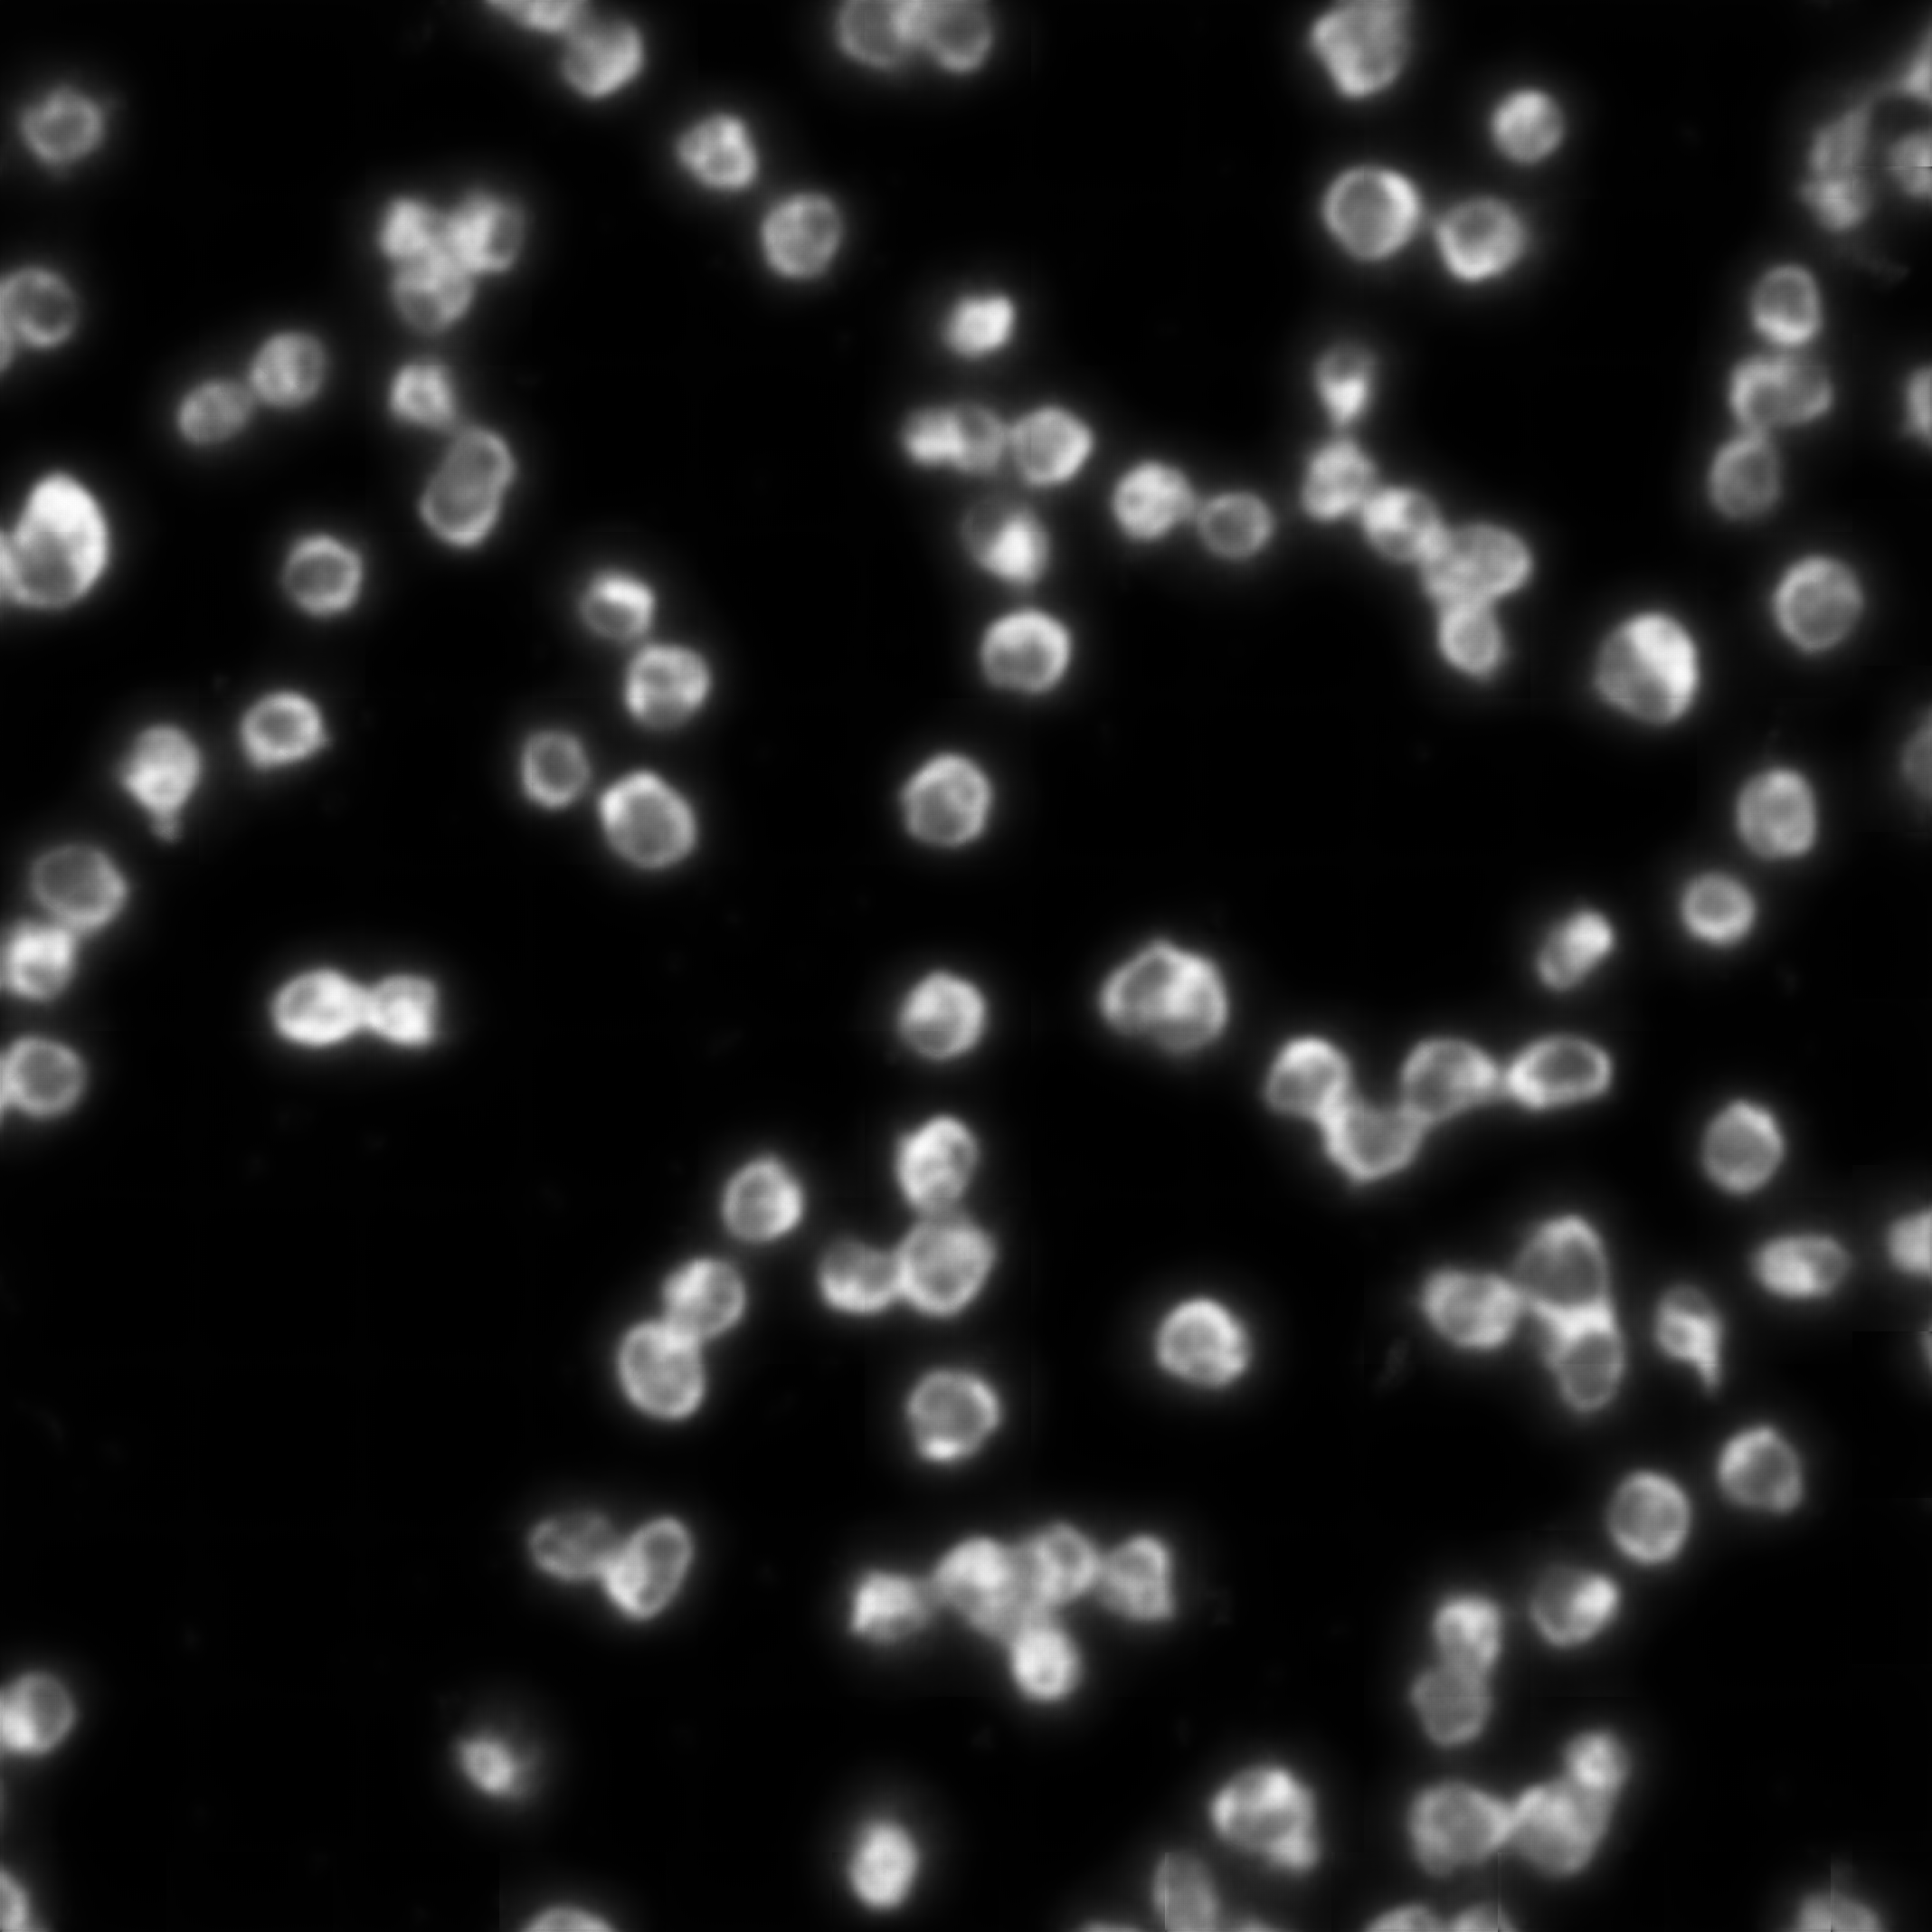
\includegraphics{bilder/ER/segmentation/pp_1.png} & 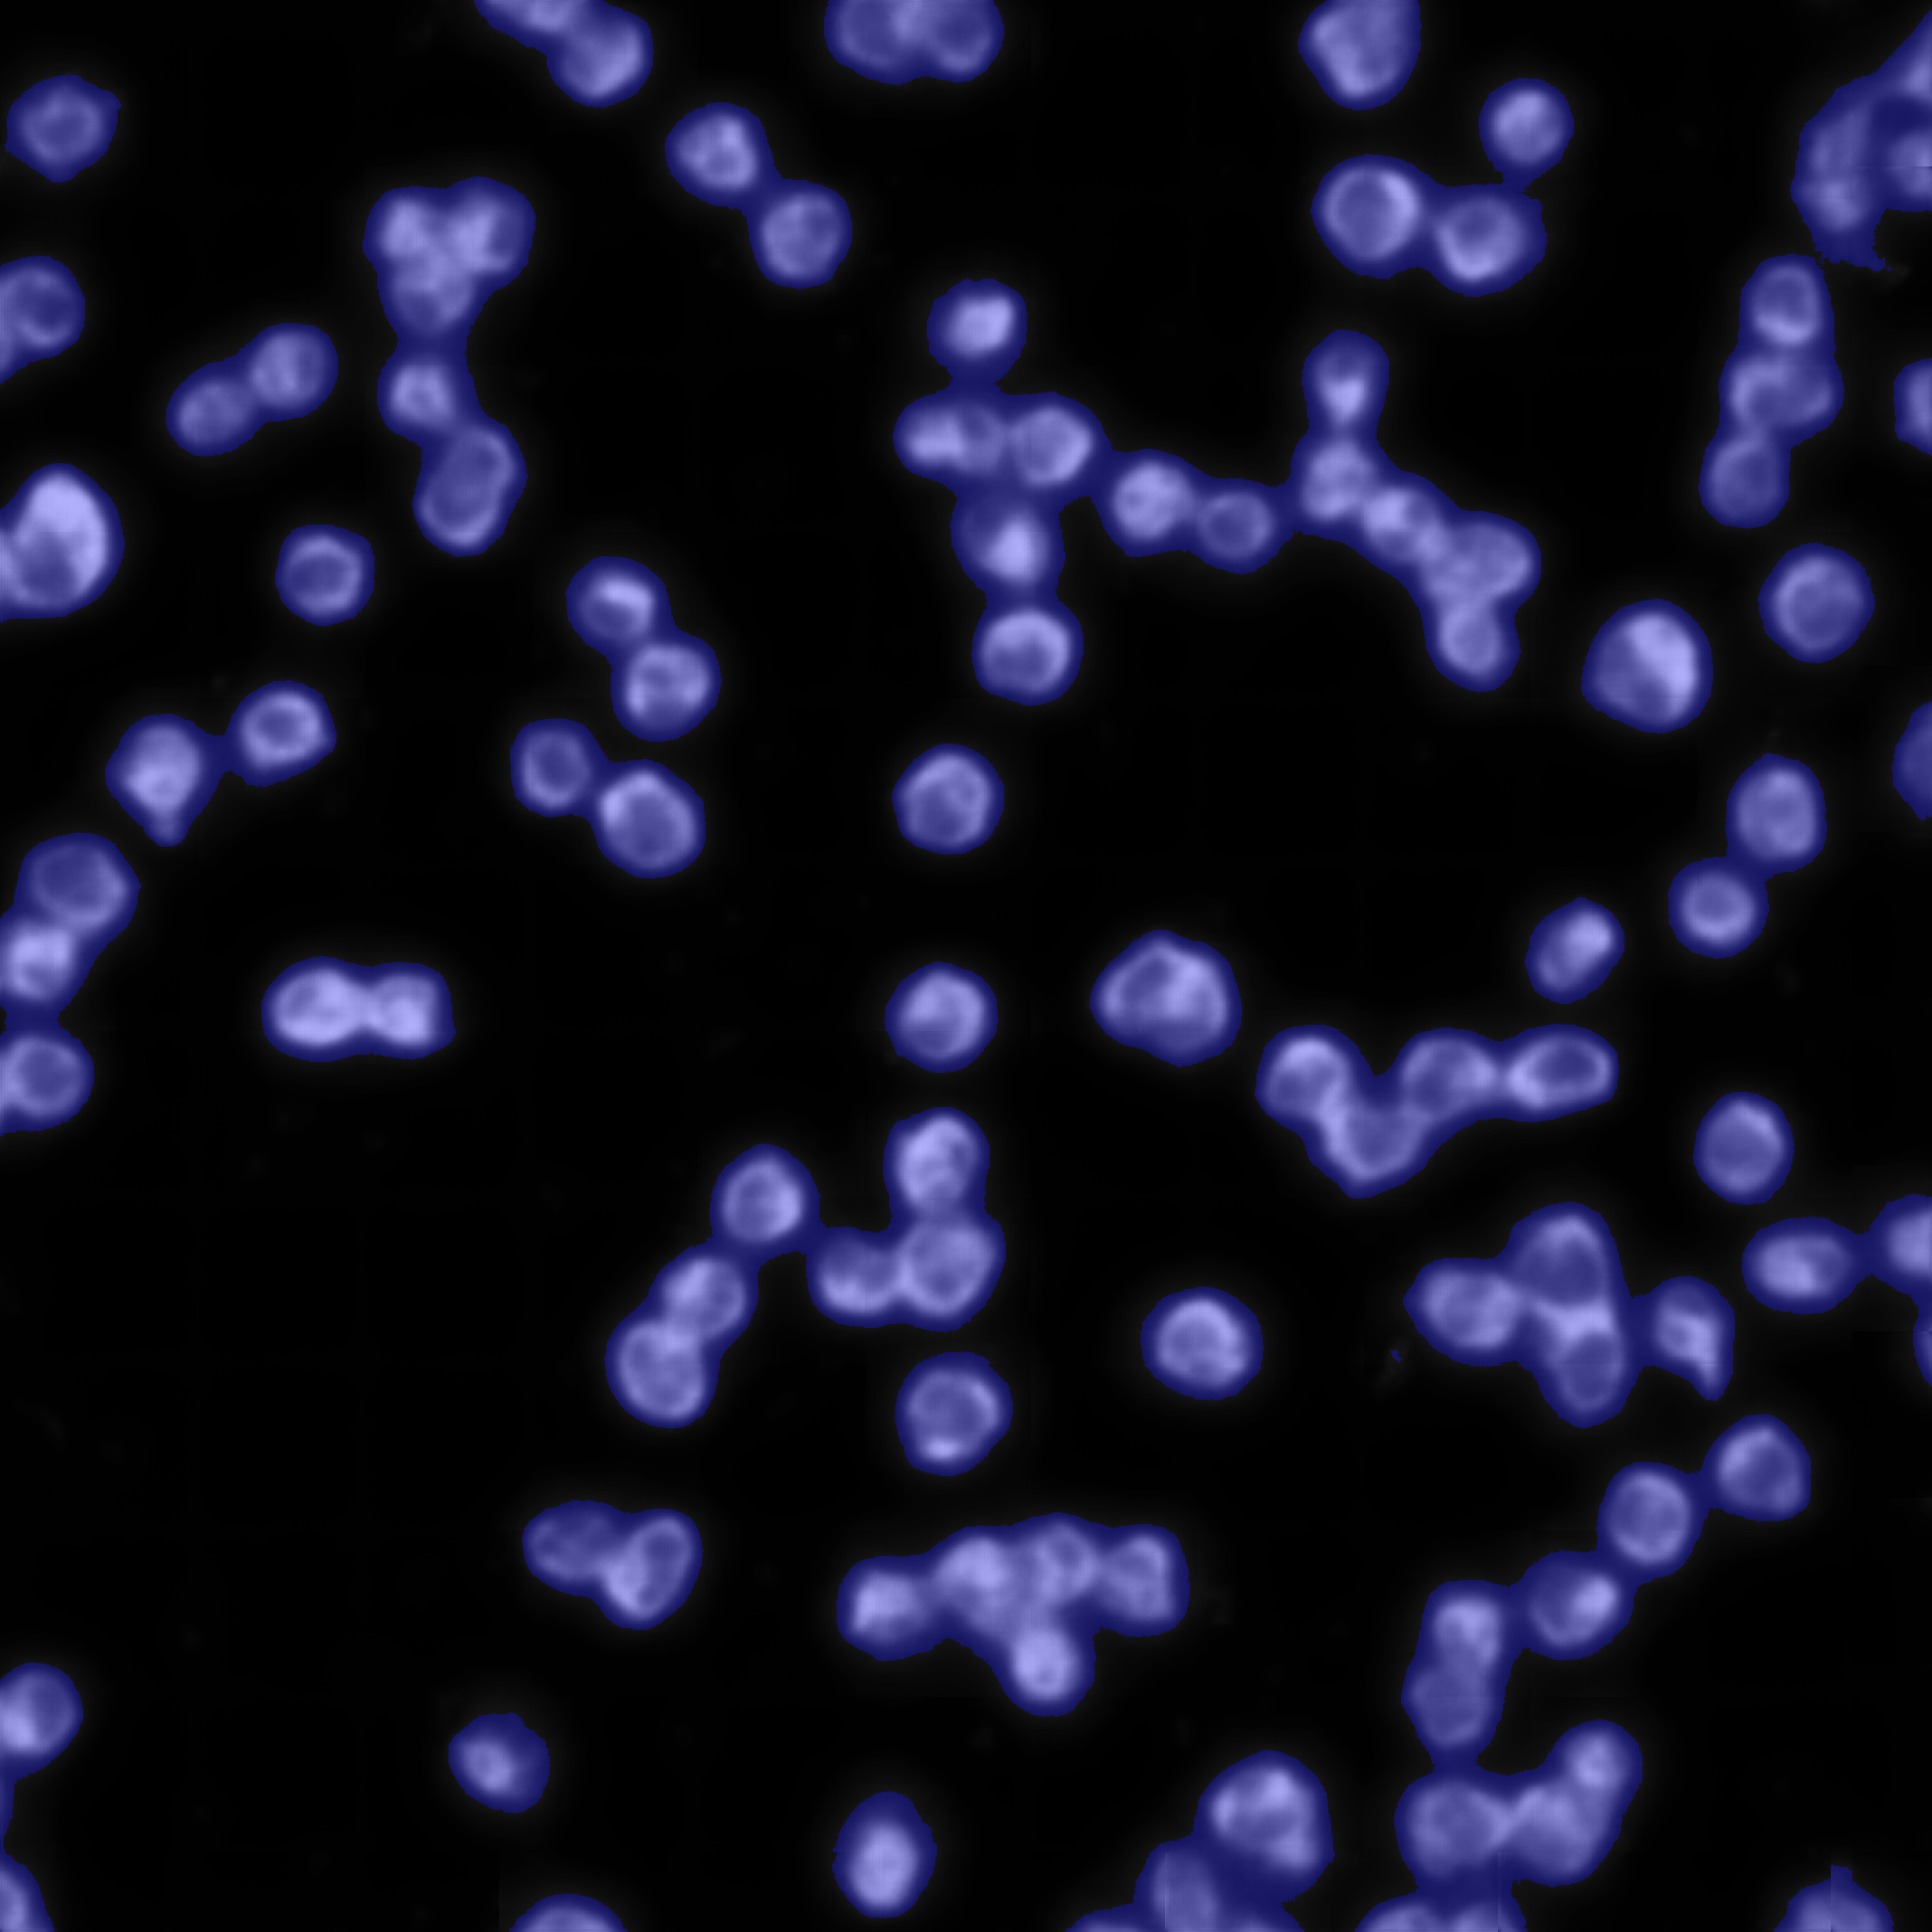
\includegraphics{bilder/ER/segmentation/pp_2.png} &
            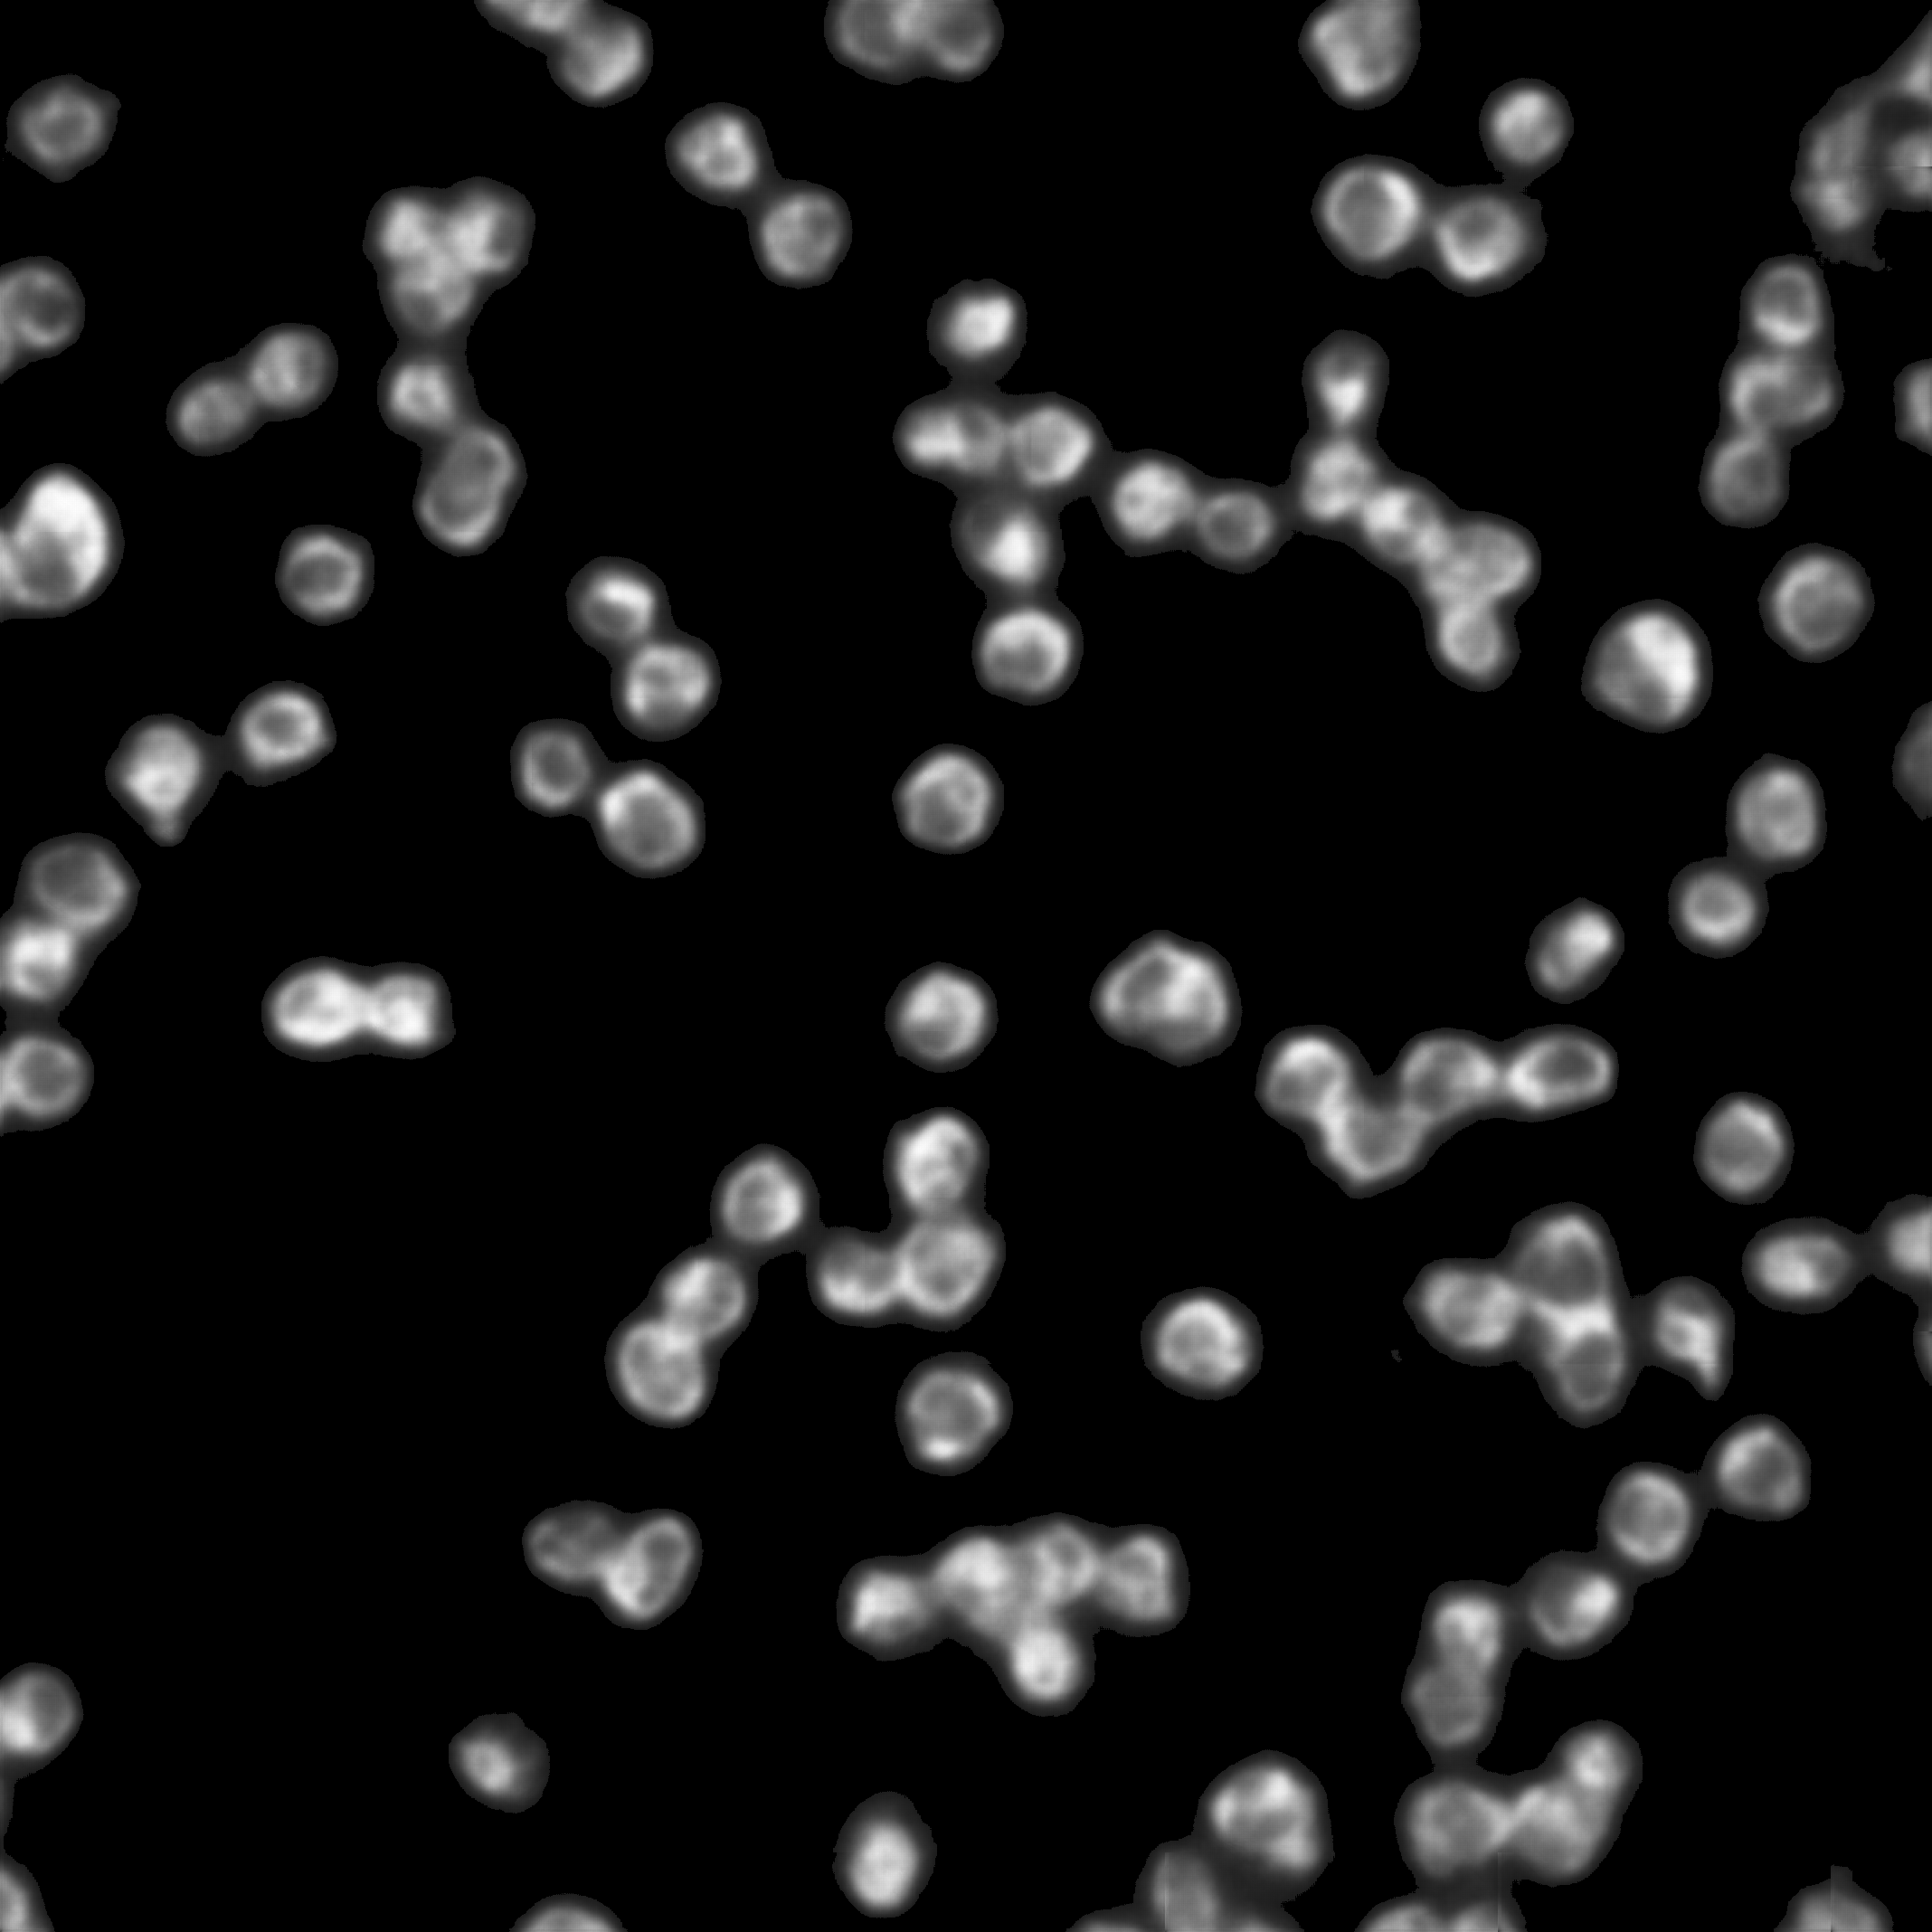
\includegraphics{bilder/ER/segmentation/pp_3.png} &
            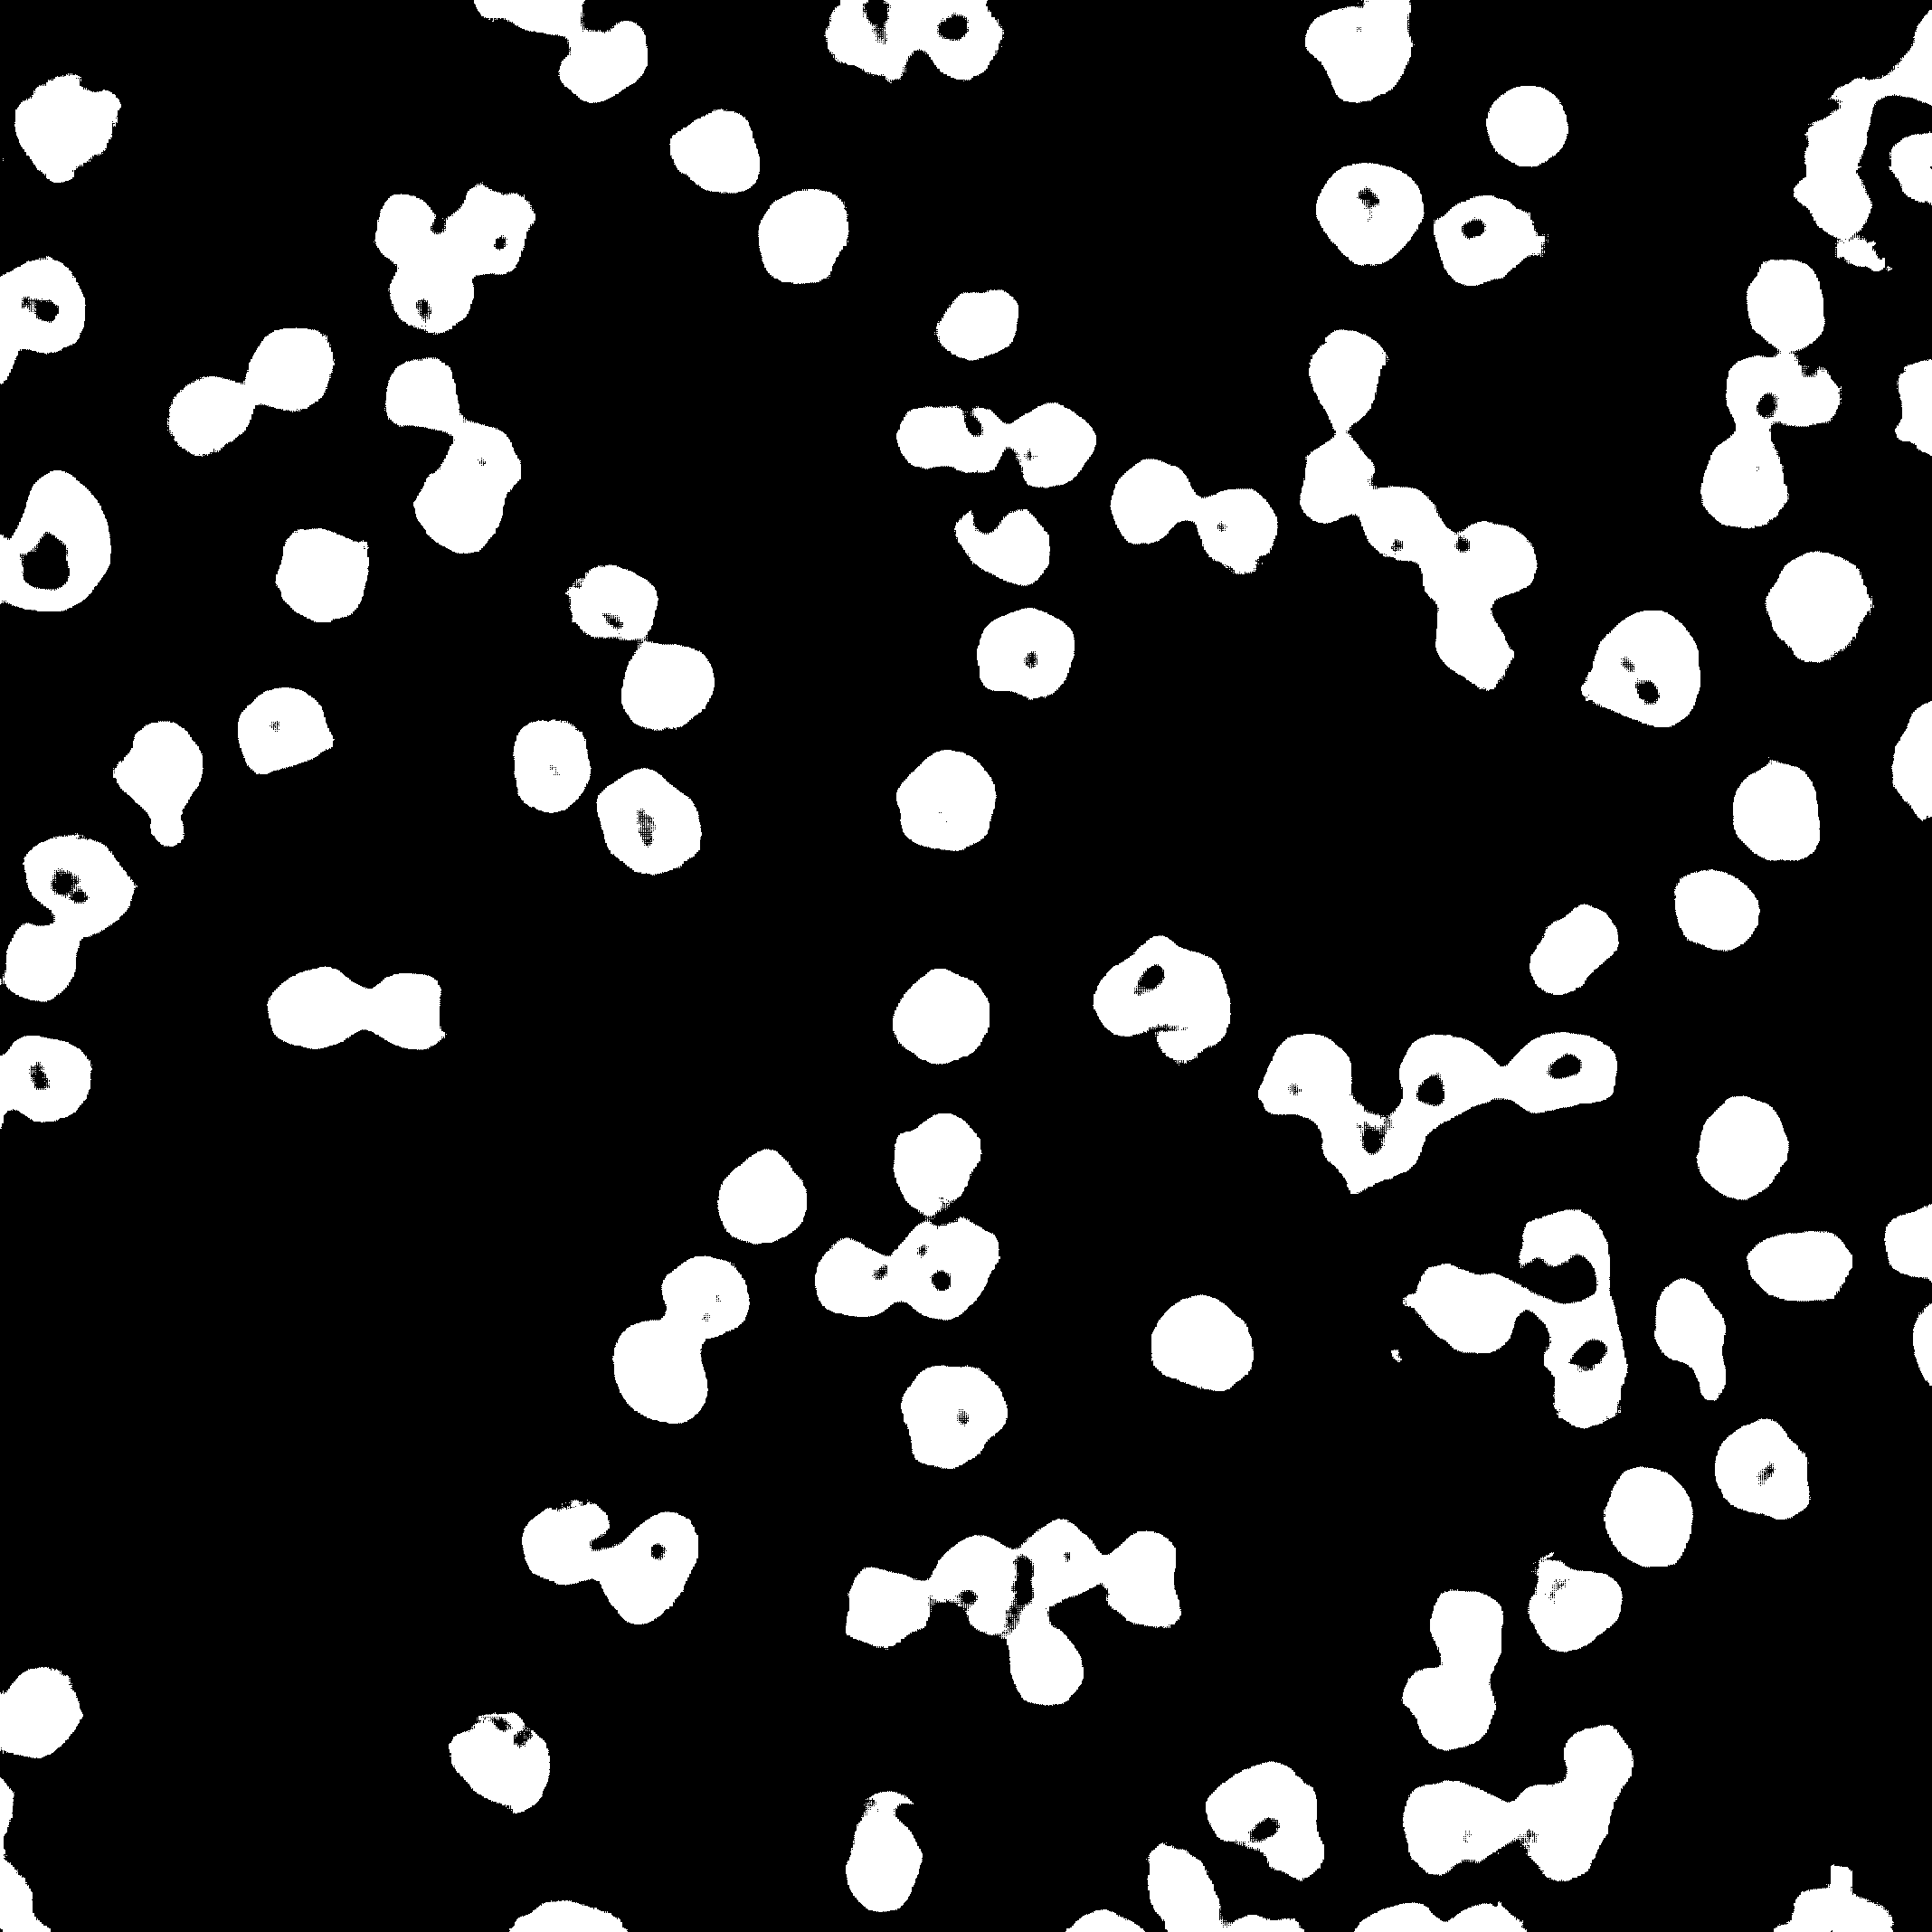
\includegraphics{bilder/ER/segmentation/pp_4.png} &
            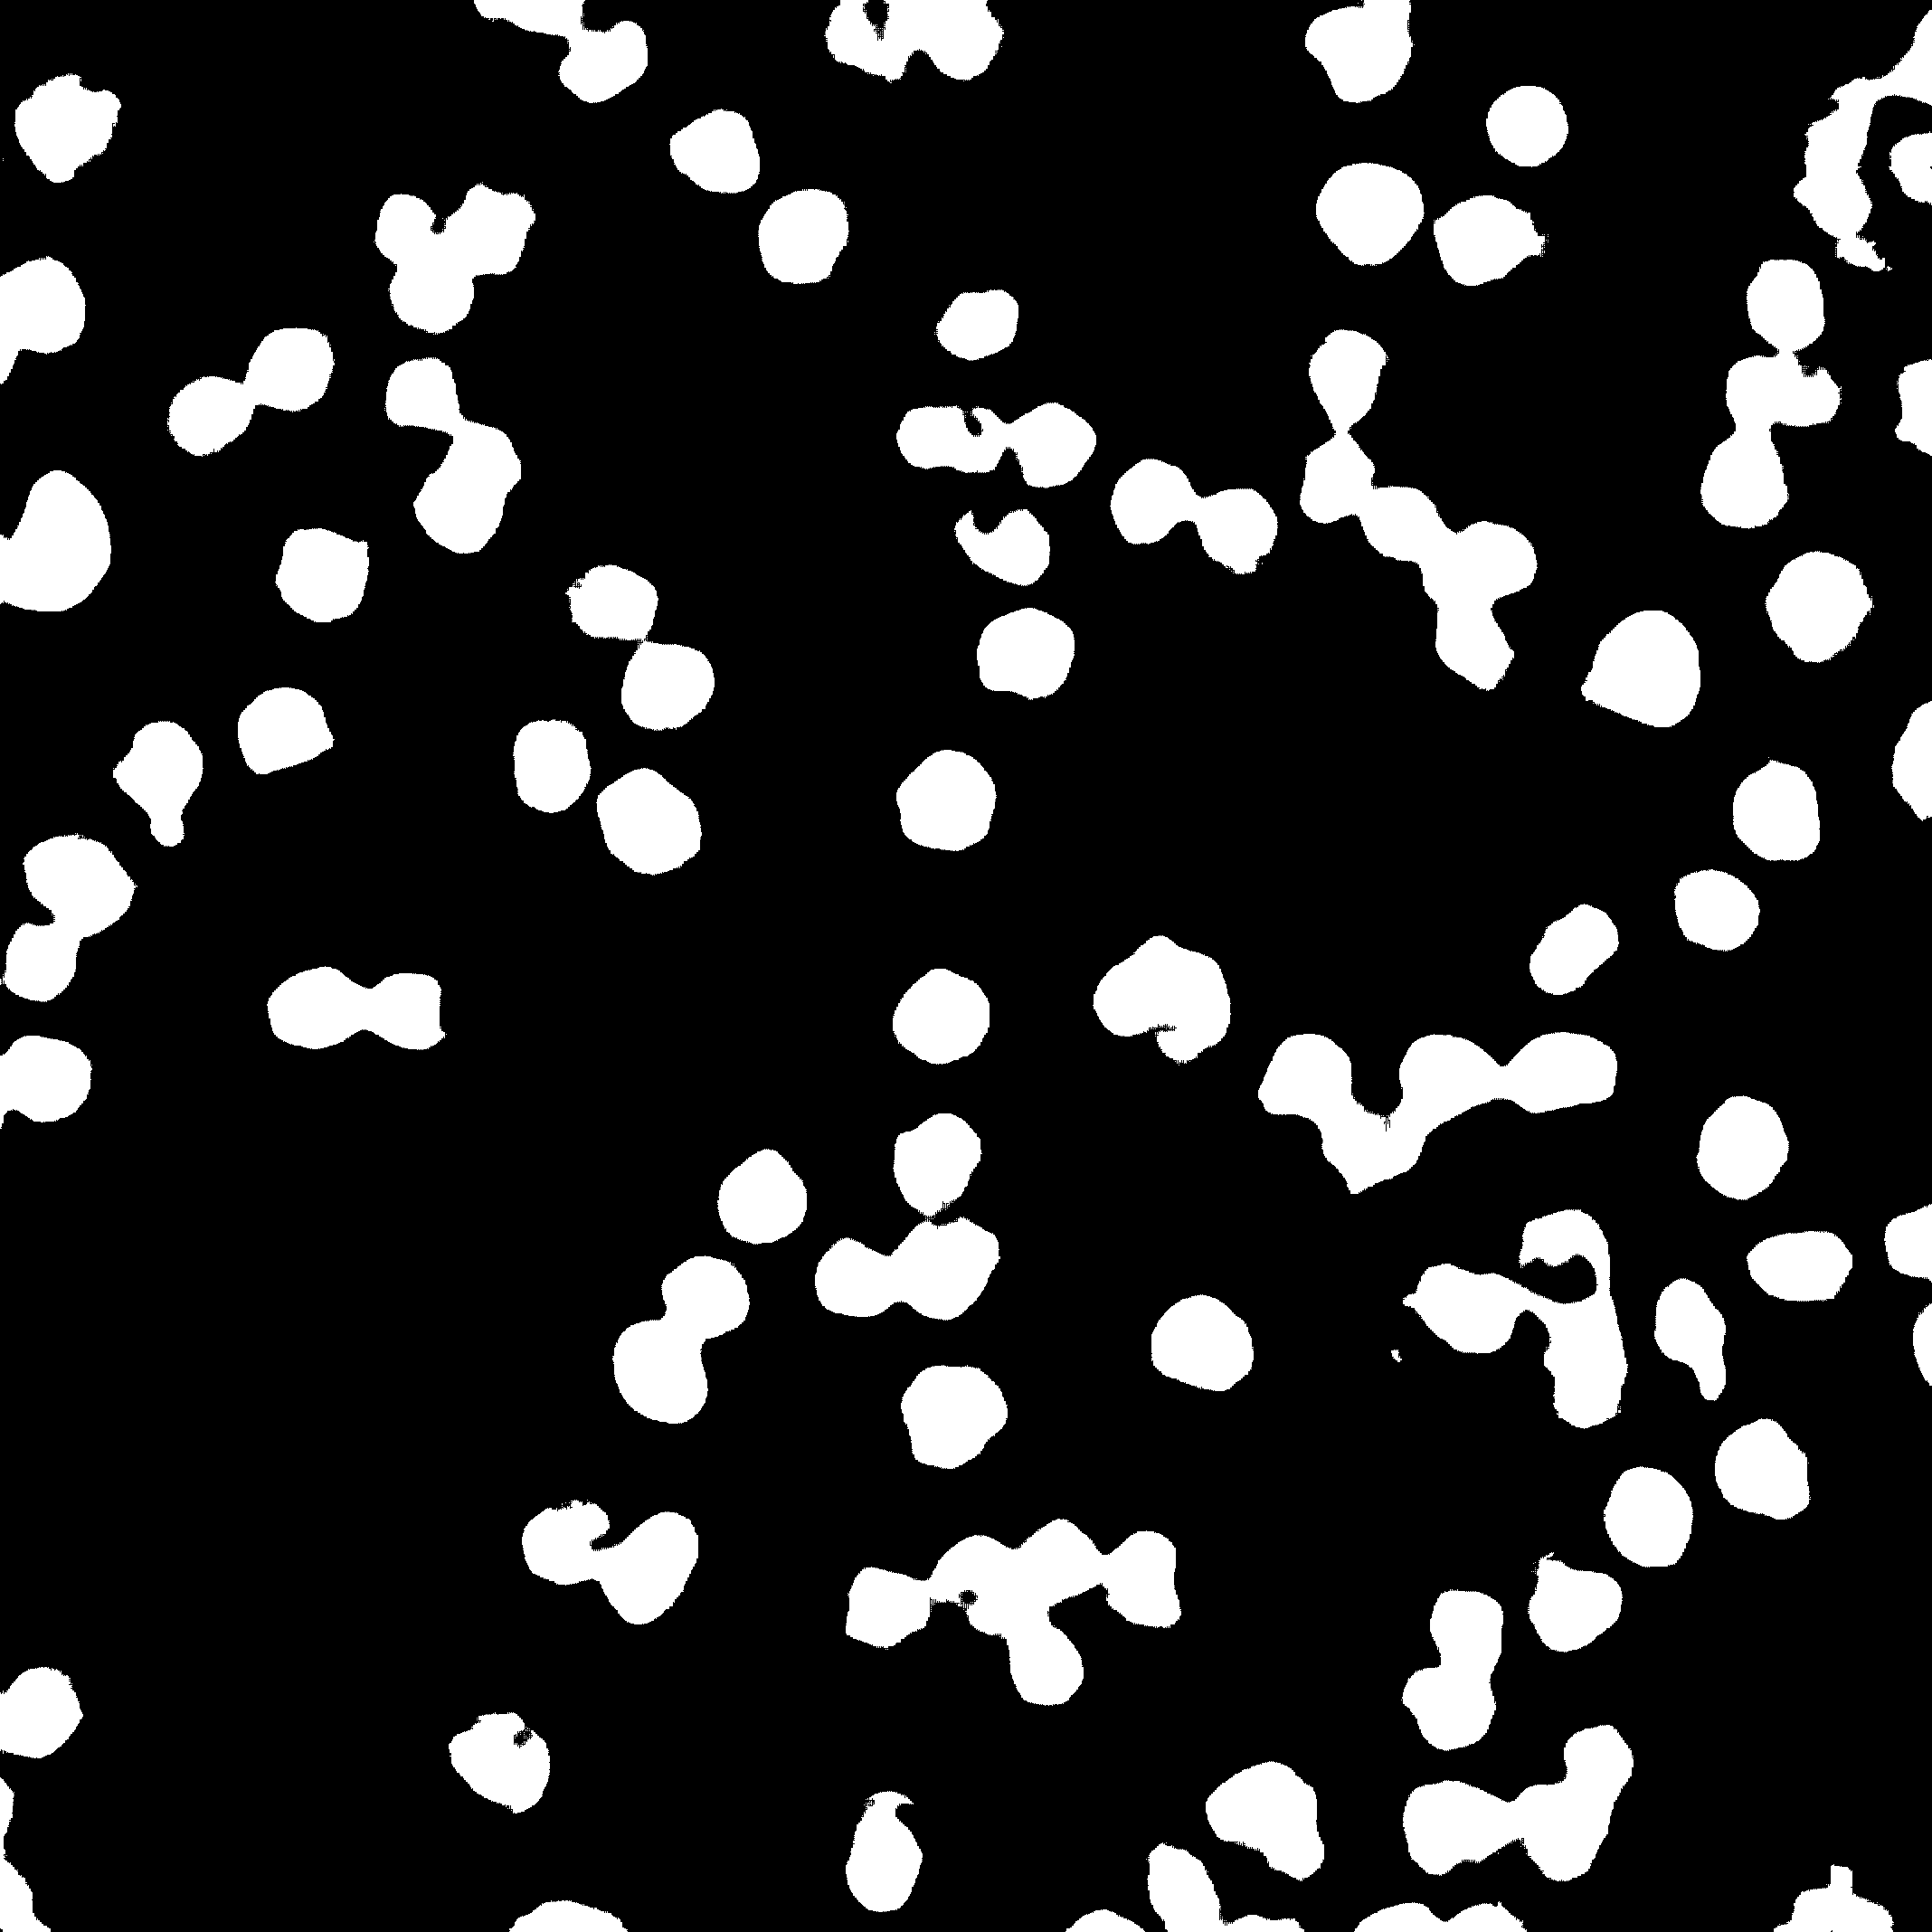
\includegraphics{bilder/ER/segmentation/pp_5.png} &
            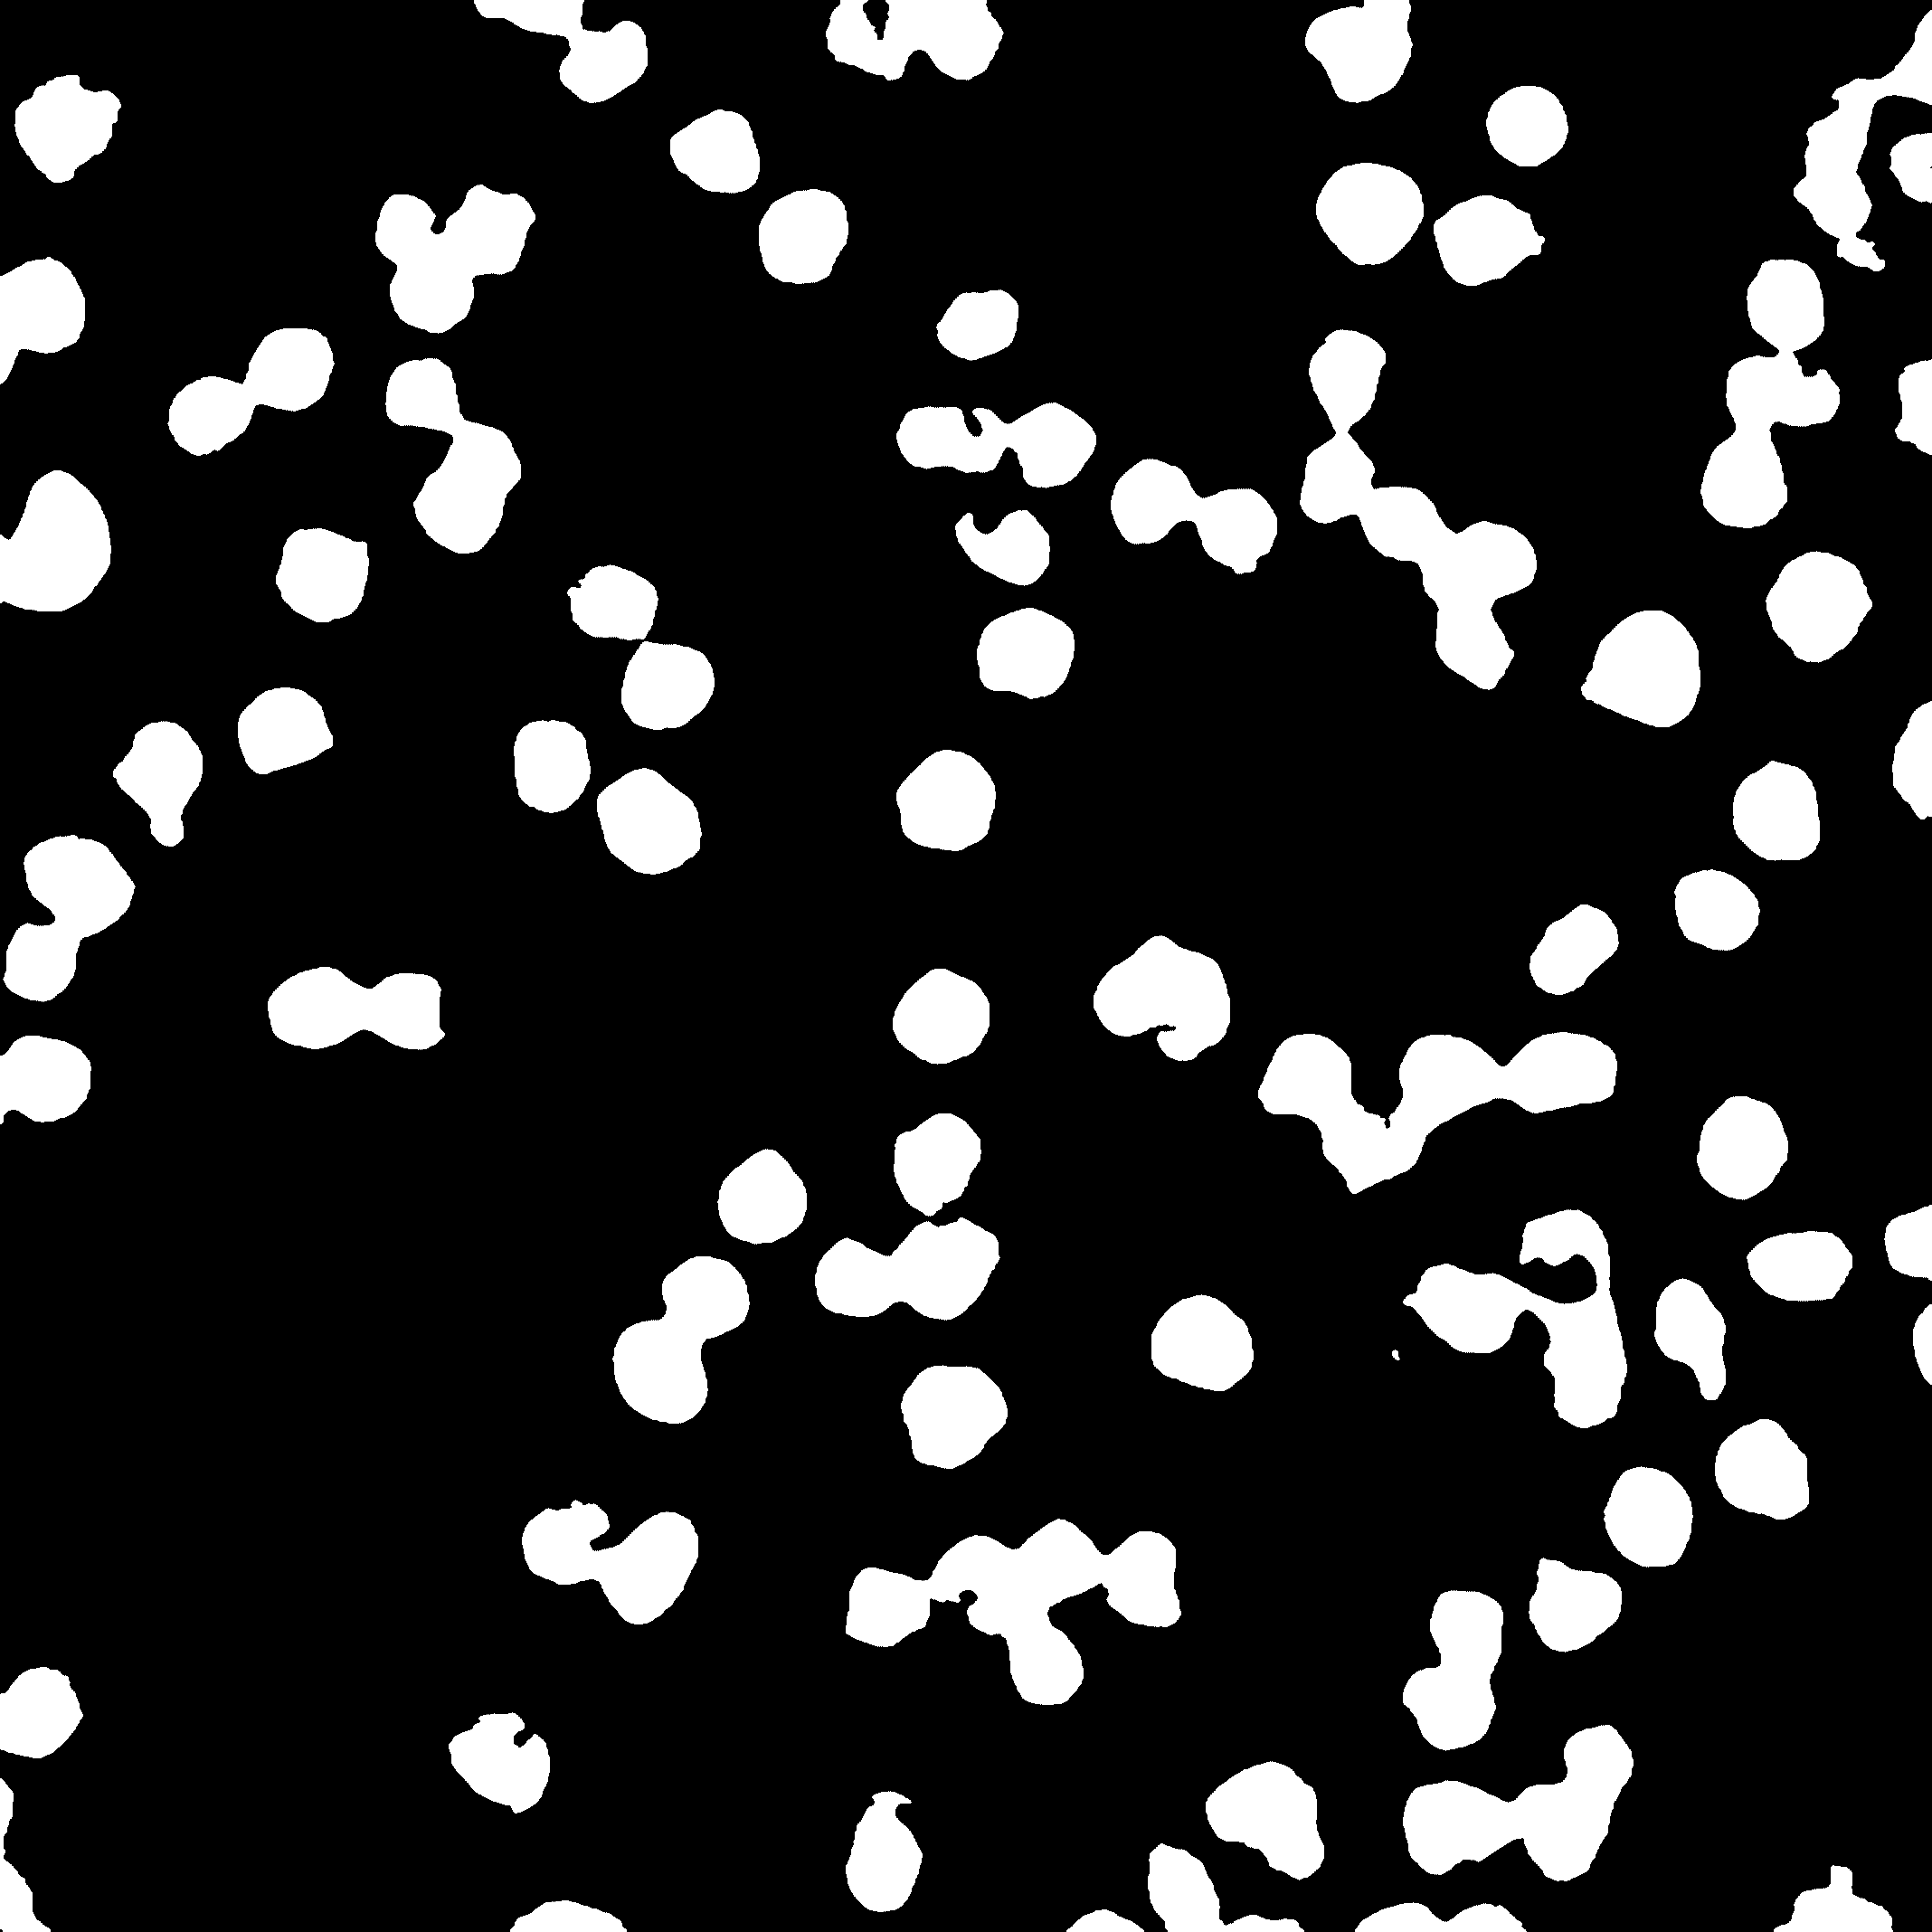
\includegraphics{bilder/ER/segmentation/pp_6.png} &
            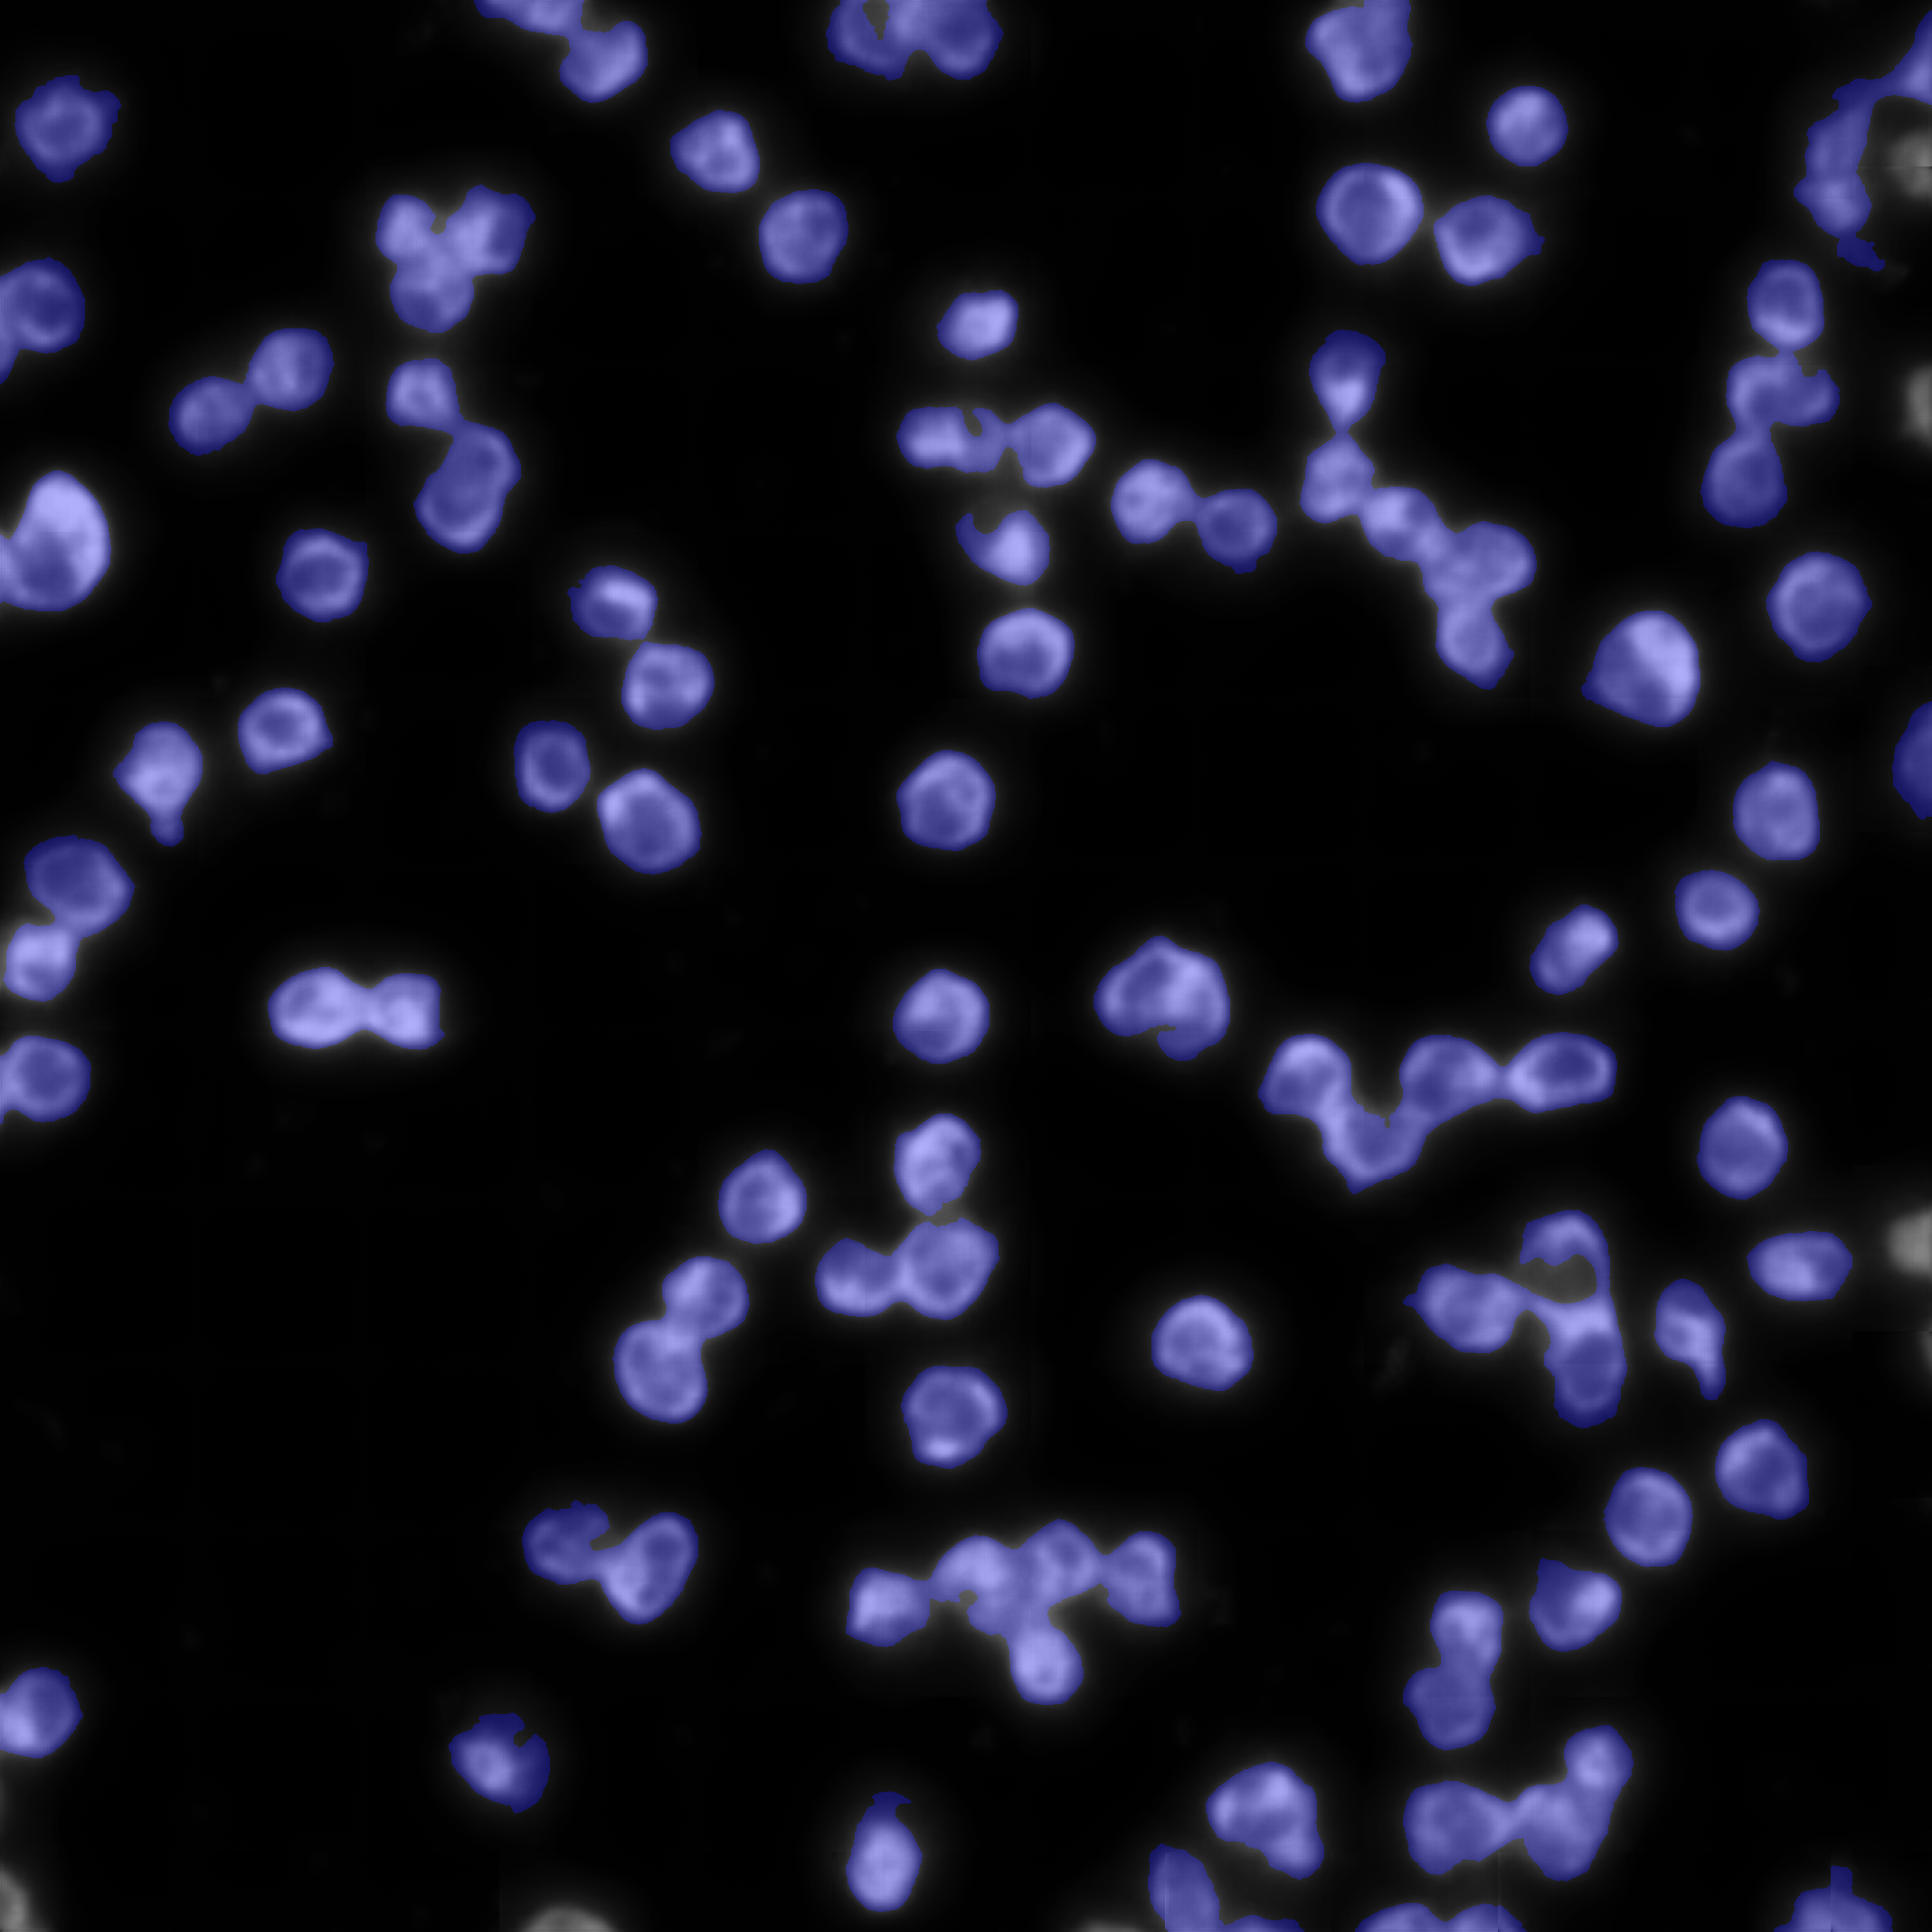
\includegraphics{bilder/ER/segmentation/pp_7.png} 
        \end{tabularx}
    \caption{ER prediction}
    \label{fig:er-prediction}
\end{figure}


\subsection{Golgi}
